\documentclass[11pt]{report}
\usepackage{fontspec}
\setmainfont{Latin Modern Roman}
\setsansfont{Latin Modern Sans}
\setmonofont{Latin Modern Mono}
\usepackage{unicode-math}
\setmathfont{Latin Modern Math}
\DeclareFontShape{TU}{LatinModernMono(0)}{b}{n}{<->ssub*LatinModernMono(0)/m/n}{}
\usepackage{pifont}
\usepackage{xcolor}
\usepackage{minted}
\usepackage{tikz}
\usepackage[vietnamese]{babel}
\usepackage[most]{tcolorbox}
\usepackage{parskip}
\usepackage{eso-pic}
\usepackage{enumitem}
\usepackage{graphicx}
\usepackage{url}
\usepackage{cite}
\usepackage{caption}
\usepackage{etoolbox}
\usepackage{tabularx}
\usepackage{multirow}
\usepackage{authblk}
\usepackage{float}
\usepackage{fancyhdr}
\usepackage[table]{xcolor}
\usepackage{colortbl}
\usepackage{xcolor}
\usepackage[dvipsnames]{xcolor}
\patchcmd{\tableofcontents}{\thispagestyle{plain}}{\thispagestyle{empty}}{}{}
\usepackage[a4paper,top=2cm,bottom=2cm,left=3cm,right=2cm,marginparwidth=1.75cm,headheight=18pt]{geometry}
\usepackage[hypertexnames=false, colorlinks=true, allcolors=teal]{hyperref}

% ========================================================================================================

\newcommand{\vekhung}{
    \begin{tikzpicture}[remember picture, overlay]
        \draw[line width=1.5pt] 
            ([shift={(3.0cm,-2.0cm)}]current page.north west) 
            rectangle ([shift={(-2.0cm,2.0cm)}]current page.south east);
        \draw[line width=0.5pt] 
            ([shift={(3.15cm,-2.15cm)}]current page.north west) 
            rectangle ([shift={(-2.15cm,2.15cm)}]current page.south east);
    \end{tikzpicture}
}

% ========================================================================================================

\setminted[sql]{
    bgcolor=teal!5,      
    fontsize=\small,
    breaklines=true,
    breakanywhere=true,
    frame=leftline,
    rulecolor=\color{teal},
    framerule=2.5pt,
    framesep=6pt,
    linenos=true,
    numbersep=5pt,
    tabsize=4,
    xleftmargin=12pt
}

% ========================================================================================================

\pagestyle{fancy}
\fancyhf{}
\lhead{\footnotesize Khoa Toán - Tin | Đại học Bách khoa Hà Nội}
\rhead{\footnotesize Nguyễn Đức Thành - 202419099}
\lfoot{\footnotesize Thiết kế Hệ thống vận chuyển hàng hóa cho Công ty vận tải}
\rfoot{\thepage}
\renewcommand{\headrulewidth}{0.4pt}
\renewcommand{\footrulewidth}{0.4pt}
\makeatletter
\let\ps@plain\ps@fancy
\makeatother

% ========================================================================================================

\begin{document}
\begin{titlepage}
    \AddToShipoutPicture*{\vekhung}
    \begin{center}
        \vspace*{6pt}
        \textbf{\Large ĐẠI HỌC BÁCH KHOA HÀ NỘI} \\
        \vspace{6pt}
        \textbf{\large Khoa Toán - Tin} \\ 
        \vspace{18pt}
        \includegraphics[width=0.3\textwidth]{LogoHUST.png} \\
        \vspace{30pt}
        \textbf{\Large BÁO CÁO BÀI TẬP LỚN} \\
        \vspace{12pt}
        \textbf{\Huge CƠ SỞ DỮ LIỆU} \\
        \vspace{12pt}
        \textbf{\Huge (MI3090)} \\
        \vspace{12pt}
        \textbf{\Large Đề tài:} \\
        \vspace{6pt}
        \textbf{\huge Thiết kế Hệ thống vận chuyển} \\ 
        \vspace{6pt}
        \textbf{\huge hàng hóa cho Công ty vận tải} \\
        \vspace{18pt}
        \begin{tabular}{ll}
            \textbf{Giảng viên hướng dẫn:} & TS. Nguyễn Thị Thanh Huyền \\
            \textbf{Sinh viên thực hiện:} & Nguyễn Đức Thành \\
            \textbf{Mã số sinh viên:} & 202419099 \\
            \textbf{Nhóm:} & 60 \\
            \textbf{Mã lớp học:} & 169309 \\
        \end{tabular} \\
    \vspace{123pt}
    \textbf{Hà Nội, Tháng 6 2026}
    \end{center}
\end{titlepage}

% ========================================================================================================

\newpage
\chapter*{Lời mở đầu}
\thispagestyle{empty}
\addcontentsline{toc}{chapter}{Lời mở đầu}
Ngành vận tải và logistics đóng vai trò huyết mạch trong nền kinh tế hiện đại. Tại Việt Nam, ngành logistics đã đạt giá trị thị trường lên tới 80,65 tỷ USD vào năm 2024 và dự kiến tăng trưởng với tốc độ CAGR 6,40\% trong giai đoạn 2025 -- 2034, đóng góp khoảng 5,17\% GDP cả nước~\cite{researchmarkets2024vietnam}. Tuy nhiên, chi phí logistics tại Việt Nam hiện vẫn ở mức cao, chiếm tới 18\% GDP, một phần do các doanh nghiệp vận tải còn hạn chế trong ứng dụng công nghệ thông tin vào quản lý hoạt động~\cite{bcompany2025vietnam}. Trong bối cảnh đó, việc xây dựng một hệ thống quản lý thông tin vận chuyển hàng hóa hiệu quả, được nền tảng hóa bởi một cơ sở dữ liệu thiết kế tốt, là nhu cầu cấp thiết đối với mọi công ty vận tải muốn nâng cao năng lực cạnh tranh.

Xuất phát từ yêu cầu của môn học \textbf{Cơ sở dữ liệu (MI3090)}, tác giả lựa chọn phát triển chủ đề \textit{``Quản lý ở một Công ty vận tải''} thành đề tài \textit{``Thiết kế Hệ thống vận chuyển hàng hóa cho Công ty vận tải''} với mục tiêu vận dụng tổng hợp các kiến thức đã học vào một dự án có tính thực tiễn. Đây không đơn thuần là một bài tập thiết kế cơ sở dữ liệu thông thường --- đề tài đặt ra yêu cầu thiết kế một hệ thống hoàn chỉnh, bao gồm nghiên cứu về quy trình nghiệp vụ, thiết kế cơ sở dữ liệu bằng cách ánh xạ từ mô hình thực thể liên kết sang mô hình quan hệ, vận dụng lý thuyết thiết kế cơ sở dữ liệu quan hệ để chuẩn hóa bản thiết kế đã đạt được từ mô hình thực thể liên kết.

Báo cáo này trình bày toàn bộ quá trình phân tích, thiết kế và cài đặt một hệ thống cơ sở dữ liệu phục vụ nghiệp vụ vận chuyển hàng hóa cho một công ty vận tải trong nước. Quy trình thiết kế tuân theo phương pháp luận chuẩn, bắt đầu từ việc xây dựng mô hình thực thể liên kết (Entity-Relationship Model --- ERD) theo đề xuất của Chen~\cite{chen1976entity}, sau đó ánh xạ sang mô hình quan hệ và chuẩn hóa theo lý thuyết phụ thuộc hàm, như đã được trình bày một cách hệ thống trong công trình kinh điển của Elmasri và Navathe~\cite{elmasri2015fundamentals}. Bố cục báo cáo được tổ chức như sau: Chương~\ref{chap:gioithieu} giới thiệu bài toán, yêu cầu dữ liệu và chức năng; Chương~\ref{chap:quytrinh} mô tả các quy trình nghiệp vụ và biểu mẫu liên quan; Chương~\ref{chap:erd} trình bày mô hình thực thể liên kết; Chương~\ref{chap:thietke} trình bày toàn bộ quá trình thiết kế và chuẩn hóa cơ sở dữ liệu quan hệ; Chương~\ref{chap:sql} trình bày các câu truy vấn SQL minh họa; Chương~\ref{chap:tsql} tự nghiên cứu về T-SQL và bảo mật cơ sở dữ liệu.

Tác giả xin được gửi lời cảm ơn chân thành đến \textbf{TS. Nguyễn Thị Thanh Huyển} --- giảng viên hướng dẫn môn Cơ sở dữ liệu --- vì những bài giảng sâu sắc và những góc nhìn thực tiễn đã định hướng cho tác giả trong suốt quá trình thực hiện đề tài. Dù đã cố gắng hết sức, báo cáo chắc chắn còn nhiều điểm cải thiện; tác giả rất mong nhận được sự góp ý từ cô để hoàn thiện hơn trong tương lai.

\vspace{21pt} 
\begin{flushright}
\begin{tabular}{c}
\textit{Hà Nội, tháng 6 năm 2026} \\
\textit{Sinh viên thực hiện} \\
\textbf{Nguyễn Đức Thành}
\end{tabular}
\end{flushright}

% ========================================================================================================

\clearpage
\makeatletter
\let\ps@plain\ps@empty
\makeatother
\addcontentsline{toc}{chapter}{Danh sách hình vẽ}
\listoffigures
\makeatletter
\let\ps@plain\ps@empty
\makeatother
\clearpage

% ========================================================================================================

\clearpage
\makeatletter
\let\ps@plain\ps@empty
\makeatother
\addcontentsline{toc}{chapter}{Danh sách bảng}
\listoftables
\makeatletter
\let\ps@plain\ps@empty
\makeatother
\clearpage

% ========================================================================================================

\clearpage
\makeatletter
\let\ps@plain\ps@empty
\makeatother
\pagestyle{empty}
\tableofcontents
\thispagestyle{empty}
\makeatletter
\let\ps@plain\ps@fancy
\makeatother
\clearpage

% ========================================================================================================

\pagestyle{fancy}

% ========================================================================================================
% CHƯƠNG 1: GIỚI THIỆU
% ========================================================================================================

\chapter{Giới thiệu bài toán}
\label{chap:gioithieu}

% ========================================================================================================

\section{Bối cảnh}
\label{sec:boicanh}

Hiện nay, trên toàn quốc có tổng chiều dài đường bộ 595.201 km, trong đó, đường bộ quốc gia (quốc lộ, cao tốc) là 25.560 km. Hệ thống kết cấu đường bộ quốc gia được quy hoạch mạng lưới đường bộ Việt Nam thời kỳ 2021 -- 2030 và tầm nhìn đến năm 2050 theo Quyết định số 1454/QĐ-TTg ngày 01/9/2022 quy hoạch mạng lưới đường bộ đảm bảo kết nối thuận lợi các trung tâm kinh tế, cảng biển, cửa khẩu,... và hệ thống quốc lộ được phân bổ theo các trục dọc, trục ngang, trục hướng tâm tạo thành các hành lang vận tải. Tính đến tháng 6/2022, mạng lưới đường cao tốc đã đưa vào khai thác khoảng 23 đoạn tuyến, tương đương với 1.239 km; đang triển khai xây dựng khoảng 14 tuyến, đoạn tuyến, tương đương với 840 km~\cite{BaoCaoLogistics2022}. 

\begin{table}[H]
    \rowcolors{2}{teal!5}{white}
    \centering
    \renewcommand{\tabularxcolumn}[1]{m{#1}}
    \begin{tabularx}{\textwidth}{|>{\raggedright\arraybackslash}m{4.3cm}|>{\raggedright\arraybackslash}X|>{\raggedright\arraybackslash}X|>{\raggedright\arraybackslash}X|>{\raggedright\arraybackslash}X|} \hline
        \rowcolor{teal!30}
        \textbf{Vùng} & \textbf{Diện tích \((km^2)\)} & \textbf{Dân số} (\textit{1000 người}) & \textbf{Chiều dài cao tốc \((km)\)} & \textbf{Chiều dài quốc lộ \((km)\)} \\ \hline
        Trung du và miền núi phía Bắc        & 95.264 & 12.569 & 396 & 7.256 \\ \hline
        Đồng bằng sông Hồng                  & 21.068 & 22.620 & 489 & 2.133 \\ \hline
        Bắc Trung Bộ và Duyên hải Miền Trung & 95.876 & 20.220 & 193 & 8.366 \\ \hline
        Tây Nguyên                           & 54.508 & 5.861  & 19  & 3.059 \\ \hline
        Đông Nam Bộ                          & 23.598 & 17.930 & 52  & 855 \\ \hline
        Đồng Bằng sông Cửu Long              & 40.548 & 17.283 & 90  & 2.652 \\ \hline
        \textbf{Tổng}                        & \textbf{330.863} & \textbf{96.483} & \textbf{1.239} & \textbf{24.321} \\ \hline
    \end{tabularx}
    \caption{Thống kê chiều dài đường cao tốc và quốc lộ theo vùng}
    \label{tab:thongkecaotocvaquoclo}
\end{table}

Trong bối cảnh hội nhập kinh tế toàn cầu và sự bùng nổ của thương mại điện tử, nhu cầu vận chuyển hàng hóa tại Việt Nam đang tăng trưởng mạnh mẽ. Thị trường vận tải đường bộ ghi nhận sự gia tăng đáng kể về sản lượng hàng hóa, đặc biệt trong các ngành dệt may, điện tử và hàng tiêu dùng nhanh (Bảng~\ref{tab:phantichdongluctangtruong})~\cite{mordor2024vn}. Chính phủ Việt Nam đã đầu tư lớn vào hạ tầng giao thông, số km cao tốc được hoàn thành, đưa vào khai thác trong năm 2023 lên tới 475km và tổng số đường bộ cao tốc nước ta đến thời điểm hiện nay đạt 1.892km \cite{vneconomy2025caotoc}. Điều này mở ra cơ hội lớn cho các doanh nghiệp vận tải mở rộng mạng lưới phân phối và nâng cao hiệu quả hoạt động.

\begin{table}[H]
    \rowcolors{2}{teal!5}{white}
    \centering
    \renewcommand{\tabularxcolumn}[1]{m{#1}}
    \begin{tabularx}{\textwidth}{|>{\raggedright\arraybackslash}X|c|>{\raggedright\arraybackslash}X|>{\raggedright\arraybackslash}l|} \hline
        \rowcolor{teal!30}
        \textbf{Yếu tố thúc đẩy} & \textbf{CAGR} & \textbf{Khu vực ảnh hưởng} & \textbf{Thời gian tác động} \\ \hline
        Xu hướng dịch chuyển sản xuất (Near-shoring) vào Việt Nam                       & \(+1.8\%\) & Bắc Ninh, Thái Nguyên, Đồng Nai, Bình Dương   & Trung hạn (2-4 năm) \\ \hline
        Sự bùng nổ của bưu kiện Thương mại điện tử (B2C \& C2C)                         & \(+1.2\%\) & TP. Hồ Chí Minh, Hà Nội, Đà Nẵng              & Ngắn hạn ($\le$ 2 năm) \\ \hline 
        Số hóa hải quan theo cơ chế "Một cửa" ASEAN                                     & \(+0.9\%\) & Các cảng chính và cửa khẩu                    & Trung hạn (2-4 năm) \\ \hline
        Mở rộng hành lang vận tải đường bộ xuyên biên giới Trung Quốc - Lào - Campuchia & \(+0.7\%\) & Lạng Sơn, Quảng Ninh, Đồng bằng sông Cửu Long & Dài hạn ($\ge$ 4 năm) \\ \hline
    \end{tabularx}
    \caption{Phân tích động lực tăng trưởng (Drivers Impact Analysis)}
    \label{tab:phantichdongluctangtruong}
\end{table}

Tuy nhiên, phần lớn các công ty vận tải vừa và nhỏ tại Việt Nam vẫn đang quản lý đơn hàng, phân công phương tiện và theo dõi hàng hóa theo phương thức thủ công hoặc trên các hệ thống rời rạc, thiếu tính liên kết. Điều này dẫn đến nhiều vấn đề thực tế: thông tin bị phân mảnh, khó truy vết hàng hóa theo thời gian thực, sai sót trong thanh toán và lập hóa đơn, đồng thời gây khó khăn cho việc phân tích hiệu quả hoạt động. Nghiên cứu của Bazaras và đồng nghiệp chỉ ra rằng việc tích hợp thông tin trong vận chuyển đa phương thức đòi hỏi một hệ thống quản lý dữ liệu có cấu trúc chặt chẽ, đảm bảo tính chính xác và đồng bộ của thông tin giữa tất cả các bên tham gia~\cite{bazaras2024multimodal}.

Thực trạng đó đặt ra yêu cầu cấp thiết phải xây dựng một hệ thống quản lý thông tin vận chuyển hàng hóa chuyên biệt, có khả năng số hóa toàn bộ quy trình nghiệp vụ, từ tiếp nhận đơn hàng, lập lộ trình vận chuyển, theo dõi hàng hóa thời gian thực đến thanh toán và báo cáo, nhằm nâng cao hiệu quả hoạt động và đáp ứng yêu cầu phát triển trong kỷ nguyên số.

% ========================================================================================================

\section{Lý do lựa chọn bài toán}
\label{sec:lydo}

Bài toán \textit{``Thiết kế Hệ thống Vận chuyển hàng hóa cho Công ty Vận tải''} được lựa chọn vì những lý do sau:

\begin{enumerate}
    \item \textbf{Tính thực tiễn cao:} Bài toán phản ánh trực tiếp nhu cầu số hóa đang diễn ra tại hàng nghìn doanh nghiệp vận tải Việt Nam. Tính đến năm 2022, chi phí logistics của Việt Nam chiếm tới 18\% GDP. Hiệp hội Dịch vụ Logistics Việt Nam (VLA) báo cáo rằng ngành logistics gần đây đã tăng trưởng với tốc độ khoảng 14 -- 16\%, với giá trị ngành hàng năm dao động từ 40 tỷ USD đến 42 tỷ USD~\cite{researchmarkets2024vietnam}. Theo dự báo của Bộ Công Thương, đến năm 2030, nhu cầu nguồn nhân lực logistics sẽ vượt 200.000 người, trong khi khả năng đáp ứng chỉ đạt khoảng 10\% nhu cầu thực tế~\cite{tapchicongthuong2020nhanluclogistics}. Điều này đặt áp lực ngược lại lên các hệ thống thông tin phải đủ thông minh để bù đắp sự thiếu hụt nhân lực bằng tự động hóa quy trình.
    
    \item \textbf{Tính ứng dụng học thuật của môn học:} Chủ đề này là bối cảnh lý tưởng để áp dụng toàn diện kiến thức môn Cơ sở dữ liệu vào một bài toán thực tế có đủ độ phức tạp và tính đại diện. Cụ thể, bài toán yêu cầu sinh viên thực hiện đầy đủ quy trình thiết kế từ phân tích yêu cầu nghiệp vụ, xây dựng mô hình thực thể liên kết (ERD) cho đến ánh xạ sang lược đồ quan hệ và triển khai biểu thức đại số quan hệ. Bên cạnh thiết kế cơ sở dữ liệu, đề tài còn giúp sinh viên rèn luyện kỹ năng phân tích nghiệp vụ để xác định đúng thực thể cần mô hình hóa, xây dựng truy vấn phức tạp liên quan đến JOIN nhiều bảng, subquery và aggregation, đồng thời đưa ra các quyết định thiết kế có lập luận (ví dụ: tại sao nên lưu \texttt{TONG\_TIEN} trong \texttt{HOA\_DON} thay vì tính lại từ \texttt{DON\_HANG}).

    \item \textbf{Độ phức tạp phù hợp:} Hệ thống bao gồm đầy đủ các yếu tố cần thiết để vận dụng toàn bộ kiến thức môn học: mô hình hóa dữ liệu phức tạp với nhiều thực thể và mối quan hệ, yêu cầu chuẩn hóa đến dạng chuẩn cao, và các truy vấn có ý nghĩa thực tiễn. Một trong những thách thức nghiệp vụ trọng tâm là mô hình hóa hành trình vận chuyển từ bưu cục gửi qua các điểm trung chuyển đến bưu cục nhận. Giải pháp được đề xuất thông qua thực thể \texttt{CHANG\_DUONG} với thuộc tính \texttt{STT} (số thứ tự), đóng vai trò định vị thứ tự chặng trong lộ trình, cho phép lưu trữ đầy đủ thứ tự điểm dừng và thời gian hoàn thành thực tế tại từng chặng.

    \item \textbf{Nền tảng cho phát triển tiếp theo:} Lược đồ cơ sở dữ liệu được thiết kế trong đề tài có thể triển khai trực tiếp làm nền tảng cho các ứng dụng thực tế, bao gồm phần mềm quản lý vận đơn nội bộ của công ty vận tải, ứng dụng mobile cho tài xế cập nhật trạng thái giao hàng, cổng thông tin cho khách hàng tra cứu đơn hàng, và hệ thống báo cáo doanh thu và hiệu suất vận hành. Một cơ sở dữ liệu được thiết kế tốt là nền tảng thiết yếu để tích hợp các công nghệ hiện đại như theo dõi GPS thời gian thực, tối ưu hóa tuyến đường và phân tích dữ liệu lớn~\cite{ieee2019transport}.
\end{enumerate}

% ========================================================================================================

\section{Mô tả bài toán}
\label{sec:motabaitoan}

Bài toán đặt ra là xây dựng cơ sở dữ liệu cho một công ty vận tải nội địa chuyên vận chuyển hàng hóa theo mô hình \textit{hub-and-spoke} (trung tâm -- vệ tinh), tức là hàng hóa được vận chuyển theo các lộ trình cố định, mỗi lộ trình bao gồm nhiều chặng đường nối tiếp qua các điểm trung chuyển.

Cụ thể, hệ thống cần hỗ trợ toàn bộ vòng đời của một đơn hàng vận chuyển, từ khi khách hàng đặt đơn, qua các bước lập lộ trình, phân công nhân viên và phương tiện theo từng chặng, theo dõi trạng thái hàng hóa tại từng điểm trung chuyển, cho đến khi hoàn thành giao hàng và xuất hóa đơn thanh toán.

Hệ thống được thiết kế dựa trên phương pháp luận thiết kế cơ sở dữ liệu theo mô hình thực thể liên kết (ER) do P.P. Chen đề xuất năm 1976~\cite{chen1976entity}, sau đó ánh xạ sang mô hình quan hệ và thực hiện chuẩn hóa. Phương pháp này đã được chứng minh là tạo ra các lược đồ quan hệ đạt dạng chuẩn Boyce-Codd (BCNF) trong nhiều trường hợp, đảm bảo tính toàn vẹn và không dư thừa dữ liệu~\cite{ieee1989er}.

Đề tài không đề cập đến quản lý hàng tồn kho chi tiết theo sản phẩm, hệ thống định giá cước động (dynamic pricing), tích hợp giao thông vận tải đa phương thức (đường sắt, hàng không), cũng như các chức năng thương mại điện tử hoặc giao diện người dùng cuối.

% ========================================================================================================

\section{Ý nghĩa và Ứng dụng}
\label{sec:ynghiavaungdung}

\subsection{Ý nghĩa của hệ thống}
Hệ thống đóng vai trò là xương sống thông tin của toàn bộ hoạt động vận chuyển, cho phép số hóa và tập trung hóa dữ liệu từ tất cả các điểm trong chuỗi vận chuyển. Thay vì quản lý phân tán qua nhiều file Excel và giấy tờ, doanh nghiệp có thể theo dõi trạng thái từng đơn hàng theo thời gian thực, tối ưu hóa lộ trình và phân công phương tiện, giảm thiểu sai sót trong thanh toán và đối soát, đồng thời xây dựng cơ sở dữ liệu lịch sử để phân tích và ra quyết định3.

Hệ thống mang lại trải nghiệm minh bạch hơn: khách hàng có thể theo dõi hành trình kiện hàng qua từng điểm trung chuyển, nhận thông báo thời gian giao hàng dự kiến, truy xuất lịch sử giao dịch và hóa đơn một cách đầy đủ, chính xác.

Ở tầm vĩ mô, việc doanh nghiệp vận tải áp dụng hệ thống thông tin tích hợp góp phần thực hiện các mục tiêu số hóa quản lý vận tải mà Nhà nước đã đặt ra~\cite{Hoang2025QuanLyVanTai}, tạo nền tảng cho việc chia sẻ dữ liệu với cơ quan quản lý, hỗ trợ kiểm soát tải trọng, giám sát hành trình và truy xuất trách nhiệm khi xảy ra sự cố.

\subsection{Ứng dụng thực tiễn}
Lược đồ cơ sở dữ liệu được thiết kế trong đề tài có thể triển khai trực tiếp làm nền tảng cho các ứng dụng thực tế, bao gồm phần mềm quản lý vận đơn nội bộ của công ty vận tải, ứng dụng mobile cho tài xế cập nhật trạng thái giao hàng, cổng thông tin cho khách hàng tra cứu đơn hàng, và hệ thống báo cáo doanh thu và hiệu suất vận hành.

Thiết kế theo hướng chuẩn hóa và module hóa cho phép hệ thống dễ dàng mở rộng trong tương lai, ví dụ tích hợp API với các sàn thương mại điện tử (Shopee, Lazada, TikTok Shop) để tự động nhận đơn, kết nối với hệ thống GPS để cập nhật vị trí phương tiện theo thời gian thực, tích hợp cổng thanh toán điện tử và ví điện tử, hoặc áp dụng thuật toán tối ưu hóa lộ trình (VRP – Vehicle Routing Problem) trên nền dữ liệu tọa độ bưu cục.

Đề tài cũng có giá trị như một case study thực tế trong giảng dạy môn Cơ sở dữ liệu, minh họa cách áp dụng lý thuyết ERD vào bài toán có độ phức tạp nghiệp vụ cao, bao gồm các trường hợp thiết kế đặc thù mà giáo trình thông thường ít đề cập như thực thể yếu nhiều cấp, quan hệ đa vai trò và tự liên kết phân cấp.

% ========================================================================================================

\section{Yêu cầu về dữ liệu}
\label{sec:yeucaudulieu}

Yêu cầu về dữ liệu xác định những thông tin cần phải lưu trữ, quản lý và duy trì trong cơ sở dữ liệu để hỗ trợ toàn bộ hoạt động vận chuyển. Căn cứ vào phân tích quy trình nghiệp vụ, dữ liệu được tổ chức thành 10 thực thể chính, được nhóm lại theo chức năng và vai trò trong hệ thống. Mỗi thực thể mang thông tin chi tiết về một khía cạnh của hoạt động vận tải, từ khách hàng, đơn hàng, lộ trình, hạ tầng vật lý đến nhân sự và theo dõi tài chính.

\subsection{Các thực thể chính trong hệ thống}

Dựa trên phân tích quy trình nghiệp vụ, hệ thống cần quản lý các nhóm thực thể sau:

\begin{enumerate}
    \item \textbf{Nhóm khách hàng và giao dịch:} Thực thể \texttt{KHACH\_HANG} (người gửi và/hoặc người nhận hàng) và \texttt{DON\_HANG} (yêu cầu vận chuyển được tạo ra từ giao dịch giữa khách hàng và công ty).
    
    \item \textbf{Nhóm kế hoạch vận chuyển:} Thực thể \texttt{LO\_TRINH} (tuyến đường vận chuyển từ điểm xuất phát đến đích) và \texttt{CHANG\_DUONG} (từng đoạn cụ thể trong lộ trình, nối hai điểm trung chuyển liền kề).
    
    \item \textbf{Nhóm hạ tầng vật lý:} Thực thể \texttt{DIEM\_TRUNG\_CHUYEN} (các kho/bãi trung chuyển tại các địa điểm trên tuyến đường) và \texttt{PHUONG\_TIEN} (xe tải, container được sử dụng trong vận chuyển).
    
    \item \textbf{Nhóm nhân sự và vận hành:} Thực thể \texttt{NHAN\_VIEN\_GIAO\_HANG} (tài xế và nhân viên phụ trách vận chuyển trên từng chặng) và \texttt{PHAN\_CONG} (bản ghi vận hành gắn kết nhân viên, phương tiện với chặng đường cụ thể trong một ca làm việc).
    
    \item \textbf{Nhóm theo dõi và tài chính:} Thực thể \texttt{CHI\_TIET\_VAN\_DON} (theo dõi trạng thái thực tế của từng đơn hàng trên từng phân công) và \texttt{HOA\_DON} (chứng từ thanh toán được phát sinh sau khi đơn hàng hoàn thành).
\end{enumerate}

\subsection{Yêu cầu lưu trữ thông tin}
Đối với từng thực thể, hệ thống cần lưu trữ các thông tin chi tiết được tổng hợp trong Bảng~\ref{tab:entities}.

\begin{table}[H]
    \rowcolors{2}{teal!5}{white}
    \centering
    \renewcommand{\tabularxcolumn}[1]{m{#1}}
    \begin{tabularx}{\textwidth}{|l|l|X|} \hline
        \rowcolor{teal!30}
        \textbf{STT} & \textbf{Thực thể} & \textbf{Thông tin cần lưu trữ} \\ \hline
        1  & KHACH\_HANG            & Mã Khách hàng (khóa chính), Tên Khách hàng, Email, Số điện thoại, Địa chỉ \\ \hline
        2  & DON\_HANG              & Mã Đơn hàng (khóa chính), Khối lượng, Quãng đường, Trạng thái, Phí vận chuyển, Thành tiền \\ \hline
        3  & LO\_TRINH              & Mã Lộ trình (khóa chính), Tên lộ trình, Trạng thái, Thời gian dự kiến \\ \hline
        4  & CHANG\_DUONG           & Mã Chặng đường (khóa chính), Số thứ tự trong lộ trình, Chiều dài chặng đường, Thời gian hoàn thành \\ \hline
        5  & DIEM\_TRUNG\_CHUYEN    & Mã Điểm trung chuyển (khóa chính), Tên Điểm trung chuyển, Địa chỉ, Thời gian lấy hàng \\ \hline 
        6  & PHUONG\_TIEN           & Biển số (khóa chính), Loại phương tiện, Trọng tải, Trạng thái \\ \hline
        7  & NHAN\_VIEN\_GIAO\_HANG & Mã Nhân viên (khóa chính), Tên Nhân viên, Số điện thoại, Email, Địa chỉ \\ \hline
        8  & PHAN\_CONG             & Mã Phân công (khóa chính), Ca làm việc \\ \hline
        9  & CHI\_TIET\_VAN\_DON    & Mã Vận đơn (khóa chính), Trạng thái, Thời gian nhận hàng, Thời gian giao hàng \\ \hline
        10 & HOA\_DON               & Mã Hóa đơn (khóa chính), Thời gian tạo, Thời gian hoàn thành, Tổng tiền, Trạng thái \\ \hline
    \end{tabularx}
    \caption{Tổng hợp yêu cầu lưu trữ thông tin các thực thể}
    \label{tab:entities}
\end{table}

% ========================================================================================================

\section{Yêu cầu về chức năng}
\label{sec:yeucauchucnang}

Yêu cầu về chức năng mô tả những tác vụ và hoạt động mà hệ thống cơ sở dữ liệu cần hỗ trợ để thực hiện các quy trình nghiệp vụ của công ty vận tải. Các chức năng này bao gồm quản lý khách hàng, đơn hàng, lộ trình, nhân viên, phương tiện, cũng như theo dõi vận đơn và tài chính. Ngoài ra, hệ thống cũng phải thực thi các ràng buộc và quy tắc nghiệp vụ để đảm bảo tính toàn vẹn dữ liệu và tuân thủ quy trình vận hành.

\subsection{Các chức năng nghiệp vụ cần hỗ trợ}
Hệ thống Cơ sở dữ liệu Quản lý công ty Vận tải hàng hóa được xây dựng nhằm thiết lập một hạ tầng dữ liệu đồng bộ, giúp số hóa toàn bộ quy trình nghiệp vụ và tối ưu hóa hiệu suất chuỗi cung ứng. Căn cứ vào yêu cầu thực tiễn của doanh nghiệp vận tải và tham khảo mô hình  hệ thống thông tin logistics được đề xuất bởi Bazaras và đồng nghiêpk~\cite{bazaras2024multimodal}, hệ thống cơ sở dữ liệu phải hỗ trợ các chức năng sau:

\begin{enumerate}
    \item \textbf{Quản lý Khách hàng:}
    \begin{itemize}
        \item Tiếp nhận và lưu trữ thông tin Khách hàng (mã Khách hàng, tên khách hàng, email, số điện thoại và địa chỉ) và quản lý lịch sử tương tác.
        
        \item Thông qua liên kết với đơn hàng, hệ thống hỗ trợ truy xuất giao dịch, xây dựng dữ liệu khách hàng và nâng cao chất lượng dịch vụ.
    \end{itemize}
    
    \item \textbf{Quản lý Đơn hàng:}
    \begin{itemize}
        \item Mỗi Đơn hàng tham gia vào luồng vận tải sẽ được hệ thống tiếp nhận và lưu trữ thông tin cơ bản (mã Đơn hàng, COD, khối lượng, trạng thái và thành tiền).
        
        \item Tự động tính phí vận chuyển (COD) dựa trên khối lượng và quãng đường giúp phân bổ phương tiện vận chuyển với trọng tải phù hợp.
    \end{itemize}

    \item \textbf{Quản lý Lộ trình và Chặng đường:}
    \begin{itemize}
        \item Định nghĩa và lưu trữ các lộ trình vận chuyển cố định. Mỗi đơn hàng sẽ được gán với một lộ trình cụ thể dựa trên điểm xuất phát và điểm đến nhằm hỗ trợ theo dõi và tối ưu hóa quá trình vận chuyển.
        
        \item Quản lý thông tin các chặng đường và điểm trung chuyển trên từng lộ trình. Việc quản lý này giúp hệ thống kiểm soát hàng hóa trong quá trình luân chuyển giữa các khu vực.
    \end{itemize}
    
    \item \textbf{Quản lý Nhân viên giao hàng:}
    \begin{itemize}
        \item Lưu trữ và quản lý thông tin nhân sự (mã Nhân viên, tên Nhân viên, email, số điện thoại và địa chỉ).
        
        \item Tạo phân công cho từng chặng đường, gắn kết nhân viên giao hàng và phương tiện vận chuyển. Qua đó đảm bảo điều phối hiệu quả và minh bạch trong quá trình vận chuyển.
    \end{itemize}
    
    \item \textbf{Quản lý Phương tiện vận chuyển:}
    \begin{itemize}
        \item Lưu trữ và quản lý thông tin phương tiện vận chuyển (biển số xe, loại phương tiện, trọng thải, trạng thái).
        
        \item Hệ thống cho phép phân công phương tiện cho từng nhân viên giao hàng đảm bảo quá trình vận chuyển diễn ra hiệu quả (phương tiện đang hoạt động, nhân viên không trùng ca làm).
    \end{itemize}
    
    \item \textbf{Quản lý Chi tiết vận đơn:}
    \begin{itemize}
        \item Ghi nhận trạng thái thực tế của từng đơn hàng tại từng chặng đường (qua thực thể CHI\_TIET\_VAN\_DON).
        
        \item Cập nhật thời gian nhận hàng và giao hàng tại từng điểm trung chuyển.
        
        \item Truy vấn vị trí hiện tại và lịch sử di chuyển của hàng hóa.
    \end{itemize}
\end{enumerate}

\subsection{Các ràng buộc và quy tắc nghiệp vụ}
Hệ thống phải đảm bảo các ràng buộc toàn vẹn sau, xuất phát từ quy trình vận hành thực tế:

\begin{enumerate}
    \item Mỗi đơn hàng phải gắn với đúng một lộ trình, và lộ trình đó phải có ít nhất một chặng đường được xác định.
    
    \item Mỗi chặng đường phải có đúng một điểm bắt đầu và một điểm kết thúc là các điểm trung chuyển khác nhau; điểm kết thúc của chặng $i$ phải trùng với điểm bắt đầu của chặng $i+1$.
    
    \item Mỗi phân công phải gắn đúng một nhân viên và một phương tiện; phương tiện phải ở trạng thái \texttt{'Dang hoat dong'} tại thời điểm phân công.
    
    \item Một chi tiết vận đơn (tracking record) chỉ hợp lệ khi chặng đường của phân công tương ứng thuộc lộ trình mà đơn hàng đang đi theo.
    
    \item Hóa đơn chỉ được tạo khi tất cả các chi tiết vận đơn của đơn hàng đó đã đạt trạng thái \texttt{'Da giao'}.
    
    \item Tổng tiền hóa đơn là thuộc tính dẫn xuất, được tính dựa trên phí vận chuyển của các đơn hàng thuộc hóa đơn đó.
\end{enumerate}

\subsection{Sơ đồ phân rã chức năng (BFD)}
\begin{figure}[H]
    \centering
    \includegraphics[width=0.95\textwidth]{bfd.png}
    \caption{Sơ đồ phân rã chức năng}
    \label{fig:bfd}
\end{figure}

% ========================================================================================================
% CHƯƠNG 2: QUY TRÌNH NGHIỆP VỤ VÀ BIỂU MẪU
% ========================================================================================================

\chapter{Quy trình nghiệp vụ và biểu mẫu}
\label{chap:quytrinh}

Trước khi tiến hành xây dựng mô hình dữ liệu, việc phân tích kỹ lưỡng các quy trình nghiệp vụ là bước không thể bỏ qua. Theo Elmasri và Navathe~\cite{elmasri2015fundamentals}, giai đoạn thu thập và phân tích yêu cầu --- bao gồm nghiên cứu tài liệu nghiệp vụ và quan sát quy trình thực tế --- là nền tảng để xây dựng một mô hình khái niệm phản ánh đúng thực tiễn hoạt động. Chương này mô tả bốn quy trình nghiệp vụ cốt lõi và bốn biểu mẫu tương ứng của hệ thống, được xác định dựa trên sơ đồ phân rã chức năng tại Hình~\ref{fig:bfd}.

% ========================================================================================================

\section{Quy trình tiếp nhận đơn hàng vận chuyển}
\label{sec:qt_tiepnhan}

Quy trình tiếp nhận đơn hàng là điểm khởi đầu của toàn bộ chu trình vận chuyển, tương ứng với nhóm chức năng \textbf{Quản lý Khách hàng} và \textbf{Quản lý Đơn hàng} trong sơ đồ phân rã chức năng. Quy trình được thực hiện theo các bước tuần tự:

\begin{enumerate}
    \item \textbf{Tiếp nhận thông tin Khách hàng:} Nhân viên tiếp nhận ghi nhận thông tin người gửi và người nhận vào thực thể \texttt{KHACH\_HANG}, bao gồm tên (\texttt{TEN\_KH}), email (\texttt{EMAIL}), số điện thoại (\texttt{SDT}) và địa chỉ (\texttt{DIA\_CHI}). Một khách hàng có thể đồng thời đóng vai trò người gửi trong giao dịch này và người nhận trong giao dịch khác, do đó cả hai vai trò đều liên kết về cùng một thực thể \texttt{KHACH\_HANG} qua hai mối liên kết \texttt{GỬI} và \texttt{NHẬN}.
    
    \item \textbf{Xác định Lộ trình và tính phí:} Hệ thống tra cứu lộ trình (\texttt{LO\_TRINH}) phù hợp dựa trên điểm xuất phát và điểm đến. Phí vận chuyển (\texttt{COD} --- thuộc tính dẫn xuất) được tính tự động từ khối lượng hàng hóa (\texttt{KHOI\_LUONG}) và độ dài quãng đường (\texttt{QUANG\_DUONG}), giúp phân bổ phương tiện có trọng tải phù hợp.
    
    \item \textbf{Tạo Đơn hàng:} Sau khi khách hàng xác nhận, hệ thống tạo bản ghi \texttt{DON\_HANG} mới với \texttt{TRANG\_THAI} khởi tạo là \texttt{'Cho xu ly'}, đồng thời liên kết đơn hàng với lộ trình qua mối quan hệ \texttt{ĐI THEO}, N:1.
    
    \item \textbf{In phiếu tiếp nhận:} Hệ thống in phiếu tiếp nhận hàng hóa (Bảng~\ref{tab:phieutiepnhan}) làm căn cứ cho các bước xử lý tiếp theo.
\end{enumerate}

% ========================================================================================================

\section{Quy trình điều phối phương tiện và tài xế}
\label{sec:qt_dieuphoI}

Sau khi đơn hàng được tạo và lộ trình xác định, bộ phận vận hành tiến hành phân công phương tiện và nhân viên cho từng chặng đường --- tương ứng với nhóm chức năng \textbf{Quản lý Nhân viên giao hàng} và \textbf{Quản lý Phương tiện vận chuyển}. Quy trình gồm các bước:

\begin{enumerate}
    \item \textbf{Xác định nhu cầu vận tải:} Hệ thống liệt kê các chặng đường (\texttt{CHANG\_DUONG}) thuộc lộ trình của đơn hàng thông qua mối liên kết \texttt{BAO GỒM}, 1:N giữa \texttt{LO\_TRINH} và \texttt{CHANG\_DUONG}.
    
    \item \textbf{Kiểm tra năng lực:} Hệ thống truy vấn danh sách \texttt{PHUONG\_TIEN} đang ở trạng thái \texttt{'Dang hoat dong'} và có \texttt{TRONG\_TAI} phù hợp. Đồng thời kiểm tra \texttt{NHAN\_VIEN\_GIAO\_HANG} không có lịch trùng \texttt{CA\_LAM}.
    
    \item \textbf{Tạo phân công:} Quản lý tạo bản ghi \texttt{PHAN\_CONG} mới, gắn kết một nhân viên (mối liên kết \texttt{PHỤ TRÁCH}, 1:N) và một phương tiện (mối liên kết \texttt{SỬ DỤNG}, N:1) với chặng đường cụ thể (mối liên kết \texttt{ĐƯỢC}, 1:N).
    
    \item \textbf{Phát lệnh điều xe:} Hệ thống xuất lệnh điều xe (Bảng~\ref{tab:lenh_dieuxe}) và cập nhật \texttt{TRANG\_THAI} của phương tiện sang \texttt{'Dang van chuyen'}.
\end{enumerate}

% ========================================================================================================

\section{Quy trình theo dõi và cập nhật trạng thái hàng hóa}
\label{sec:qt_theodoi}

Quy trình theo dõi hàng hóa tương ứng với nhóm chức năng \textbf{Quản lý Chi tiết vận đơn} và được thực hiện liên tục trong suốt hành trình vận chuyển:

\begin{enumerate}
    \item \textbf{Ghi nhận lấy hàng:} Tại điểm trung chuyển đầu tiên, nhân viên giao hàng xác nhận đã nhận hàng. Hệ thống tạo bản ghi \texttt{CHI\_TIET\_VAN\_DON} mới liên kết với phân công tương ứng qua mối quan hệ \texttt{NẰM TRONG}, N:1, cập nhật \texttt{THOI\_GIAN\_NHAN\_HANG} và đặt \texttt{TRANG\_THAI} thành \texttt{'Dang van chuyen'}.

    \item \textbf{Cập nhật tại các điểm trung chuyển:} Khi hàng đến mỗi \texttt{DIEM\_TRUNG\_CHUYEN} trên lộ trình (điểm \texttt{KẾT THÚC LÀ} của chặng hiện tại, đồng thời là điểm \texttt{BẮT ĐẦU LÀ} của chặng tiếp theo), hệ thống ghi nhận \texttt{THOI\_GIAN\_GIAO\_HANG} cho chi tiết vận đơn của chặng vừa hoàn thành và khởi tạo chi tiết vận đơn mới cho chặng tiếp theo.

    \item \textbf{Xác nhận giao hàng thành công:} Tại điểm cuối cùng, hệ thống cập nhật \texttt{TRANG\_THAI} của \texttt{CHI\_TIET\_VAN\_DON} thành \texttt{'Da giao'}. Sau đó, hệ thống kiểm tra điều kiện kích hoạt quy trình xuất hóa đơn.
    
    \item \textbf{Xử lý ngoại lệ:} Trường hợp phát sinh sự cố cần phải Hoan tra hàng, \texttt{TRANG\_THAI} được cập nhật thành \texttt{'Hoan tra'} và bộ phận vận hành được thông báo.
\end{enumerate}

% ========================================================================================================

\section{Quy trình thanh toán và xuất hóa đơn}
\label{sec:qt_thanhtoan}

Quy trình tài chính được kích hoạt khi toàn bộ chặng đường của đơn hàng hoàn thành. Các bước thực hiện:

\begin{enumerate}
    \item \textbf{Kiểm tra điều kiện:} Hệ thống xác minh tất cả các bản ghi \texttt{CHI\_TIET\_VAN\_DON} liên kết với đơn hàng (qua mối quan hệ \texttt{CÓ}, 1:N) đều đạt \texttt{TRANG\_THAI} = \texttt{'Da giao'}. Đây là ràng buộc nghiệp vụ bắt buộc trước khi tạo hóa đơn.

    \item \textbf{Tạo hóa đơn:} Hệ thống tạo bản ghi \texttt{HOA\_DON} mới (thực thể mạnh, định danh độc lập), ghi nhận \texttt{THOI\_GIAN\_TAO} và tính \texttt{TONG\_TIEN} --- thuộc tính dẫn xuất từ \texttt{COD} và \texttt{THANH\_TIEN} của đơn hàng --- qua mối liên kết \texttt{BAO GỒM}, 1:N giữa \texttt{HOA\_DON} và \texttt{DON\_HANG}.

    \item \textbf{Thông báo và thu tiền:} Hệ thống thông báo hóa đơn đến khách hàng. Sau khi khách hàng thanh toán, hệ thống tự động cập nhật \texttt{THOI\_GIAN\_HOAN\_THANH} và \texttt{TRANG\_THAI} thành \texttt{'Da thanh toan'}.

    \item \textbf{Lưu trữ:} Hóa đơn được lưu trữ độc lập phục vụ kiểm toán, thống kê doanh thu và tra cứu công nợ theo khách hàng.
\end{enumerate}

% ========================================================================================================

\section{Các biểu mẫu nghiệp vụ}
\label{sec:bieumau}

Các biểu mẫu nghiệp vụ là công cụ trao đổi thông tin chuẩn hóa giữa các bộ phận trong công ty và giữa công ty với khách hàng. Mỗi biểu mẫu tương ứng với một sự kiện nghiệp vụ cụ thể và ánh xạ trực tiếp lên các trường dữ liệu trong lược đồ quan hệ.

\subsection{Phiếu tiếp nhận hàng hóa}
\label{subsec:phieutiepnhan}

Phiếu tiếp nhận được lập khi khách hàng đặt đơn vận chuyển, là chứng từ xác nhận trách nhiệm của công ty đối với hàng hóa được giao. Cấu trúc phiếu tiếp nhận được trình bày trong Bảng~\ref{tab:phieutiepnhan}.

\begin{table}[H]
    \rowcolors{2}{teal!5}{white}
    \centering
    \renewcommand{\tabularxcolumn}[1]{m{#1}}
    \begin{tabularx}{\textwidth}{|l|X|l|} \hline
        \rowcolor{teal!30}
        \textbf{Trường dữ liệu} & \textbf{Mô tả} & \textbf{Ánh xạ thực thể} \\ \hline
        Mã đơn hàng       & Mã định danh duy nhất của đơn hàng                                    & \texttt{\footnotesize DON\_HANG.ID\_DH} \\ \hline
        Họ tên người gửi  & Tên đầy đủ của khách hàng gửi hàng                                    & \texttt{\footnotesize KHACH\_HANG.TEN\_KH} \\ \hline
        SĐT người gửi     & Số điện thoại liên hệ người gửi                                       & \texttt{\footnotesize KHACH\_HANG.SDT} \\ \hline
        Địa chỉ lấy hàng  & Địa chỉ tại điểm lấy hàng                                             & \texttt{\footnotesize KHACH\_HANG.DIA\_CHI} \\ \hline
        Họ tên người nhận & Tên đầy đủ của khách hàng nhận hàng                                   & \texttt{\footnotesize KHACH\_HANG.TEN\_KH} \\ \hline
        SĐT người nhận    & Số điện thoại liên hệ người nhận                                      & \texttt{\footnotesize KHACH\_HANG.SDT} \\ \hline
        Địa chỉ giao hàng & Địa chỉ tại điểm giao hàng                                            & \texttt{\footnotesize KHACH\_HANG.DIA\_CHI} \\ \hline
        Khối lượng (kg)   & Khối lượng hàng hóa cần vận chuyển                                    & \texttt{\footnotesize DON\_HANG.KHOI\_LUONG} \\ \hline
        Quãng đường (km)  & Tổng quãng đường vận chuyển                                           & \texttt{\footnotesize DON\_HANG.QUANG\_DUONG} \\ \hline
        Phí vận chuyển    & Phí COD, tính từ khối lượng đơn hàng và độ dài quãng đường (dẫn xuất) & \texttt{\footnotesize DON\_HANG.COD} \\ \hline
        Tên lộ trình      & Lộ trình vận chuyển được chọn                                         & \texttt{\footnotesize LO\_TRINH.TEN\_LT} \\ \hline
        Ngày lập phiếu    & Ngày tiếp nhận đơn hàng                                               & (metadata hệ thống) \\ \hline
    \end{tabularx}
    \caption{Cấu trúc Phiếu tiếp nhận hàng hóa}
    \label{tab:phieutiepnhan}
\end{table}

\subsection{Lệnh điều xe}
\label{subsec:lenh_dieuxe}

Lệnh điều xe được phát hành bởi quản lý vận hành khi tạo phân công, là cơ sở để nhân viên giao hàng thực hiện chặng vận chuyển được giao (Bảng~\ref{tab:lenh_dieuxe}).

\begin{table}[H]
    \rowcolors{2}{teal!5}{white}
    \centering
    \renewcommand{\tabularxcolumn}[1]{m{#1}}
    \begin{tabularx}{\textwidth}{|l|X|l|} \hline
        \rowcolor{teal!30}
        \textbf{Trường dữ liệu} & \textbf{Mô tả} & \textbf{Ánh xạ thực thể} \\ \hline
        Mã phân công     & Mã định danh của phân công vận hành      & \texttt{\footnotesize PHAN\_CONG.ID\_PC} \\ \hline
        Ca làm việc      & Ca vận chuyển được phân công             & \texttt{\footnotesize PHAN\_CONG.CA\_LAM} \\ \hline
        Mã chặng đường   & Chặng đường cần thực hiện                & \texttt{\footnotesize CHANG\_DUONG.ID\_CD} \\ \hline
        Số thứ tự chặng  & Vị trí của chặng trong lộ trình          & \texttt{\footnotesize CHANG\_DUONG.STT} \\ \hline
        Điểm lấy hàng    & Điểm trung chuyển bắt đầu chặng          & \texttt{\footnotesize DIEM\_TRUNG\_CHUYEN.TEN\_DTC} \\ \hline
        Điểm giao hàng   & Điểm trung chuyển kết thúc chặng         & \texttt{\footnotesize DIEM\_TRUNG\_CHUYEN.TEN\_DTC} \\ \hline
        Mã nhân viên     & Nhân viên giao hàng được phân công       & \texttt{\footnotesize NHAN\_VIEN\_GIAO\_HANG.ID\_NV} \\ \hline
        Họ tên nhân viên & Tên đầy đủ của nhân viên                 & \texttt{\footnotesize NHAN\_VIEN\_GIAO\_HANG.TEN\_NV} \\ \hline
        Biển số xe       & Phương tiện được sử dụng cho chặng       & \texttt{\footnotesize PHUONG\_TIEN.BIEN\_SO} \\ \hline
        Loại phương tiện & Loại xe (xe tải nhỏ, xe tải lớn, \ldots) & \texttt{\footnotesize PHUONG\_TIEN.LOAI\_PT} \\ \hline
        Trọng tải (kg)   & Trọng tải tối đa của phương tiện         & \texttt{\footnotesize PHUONG\_TIEN.TRONG\_TAI} \\ \hline
        Ngày lập lệnh    & Ngày quản lý phát hành lệnh điều xe      & (metadata hệ thống) \\ \hline
    \end{tabularx}
    \caption{Cấu trúc Lệnh điều xe}
    \label{tab:lenh_dieuxe}
\end{table}

\subsection{Biên bản giao nhận hàng}
\label{subsec:bienban_giaonhan}

Biên bản giao nhận được lập tại mỗi điểm trung chuyển khi bàn giao hàng hóa giữa các phân công. Đây là chứng từ xác nhận chuỗi trách nhiệm vận chuyển và là nguồn dữ liệu đầu vào chính cho thực thể \texttt{CHI\_TIET\_VAN\_DON} (Bảng~\ref{tab:bienban_giaonhan}).

\begin{table}[H]
    \rowcolors{2}{teal!5}{white}
    \centering
    \renewcommand{\tabularxcolumn}[1]{m{#1}}
    \begin{tabularx}{\textwidth}{|l|>{\raggedright\arraybackslash}X|l|} \hline
        \rowcolor{teal!30}
        \textbf{Trường dữ liệu} & \textbf{Mô tả} & \textbf{Ánh xạ thực thể} \\ \hline
        Mã vận đơn chi tiết   & Mã định danh của chi tiết vận đơn                                                      & \texttt{\footnotesize CHI\_TIET\_VAN\_DON.ID\_VD} \\ \hline
        Mã đơn hàng           & Đơn hàng tương ứng cần theo dõi                                                        & \texttt{\footnotesize DON\_HANG.ID\_DH} \\ \hline
        Mã phân công          & Phân công thực hiện chặng này                                                          & \texttt{\footnotesize PHAN\_CONG.ID\_PC} \\ \hline
        Tên điểm trung chuyển & Địa điểm bàn giao hàng                                                                 & \texttt{\footnotesize DIEM\_TRUNG\_CHUYEN.TEN\_DTC} \\ \hline
        Thời gian nhận hàng   & Thời điểm thực tế nhận hàng tại điểm đầu chặng                                         & \texttt{\footnotesize CHI\_TIET\_VAN\_DON.THOI\_GIAN\_NHAN\_HANG} \\ \hline
        Thời gian giao hàng   & Thời điểm thực tế giao hàng tại điểm cuối chặng                                        & \texttt{\footnotesize CHI\_TIET\_VAN\_DON.THOI\_GIAN\_GIAO\_HANG} \\ \hline
        Trạng thái            & Kết quả bàn giao (\texttt{'Dang van chuyen'}, \texttt{'Da giao'}, \texttt{'Hoan tra'}) & \texttt{\footnotesize CHI\_TIET\_VAN\_DON.TRANG\_THAI} \\ \hline
        Chữ ký bên giao       & Xác nhận của nhân viên bàn giao hàng                                                   & (ngoài hệ thống cơ sở dữ liệu) \\ \hline
        Chữ ký bên nhận       & Xác nhận của nhân viên tiếp nhận hàng                                                  & (ngoài hệ thống cơ sở dữ liệu) \\ \hline
    \end{tabularx}
    \caption{Cấu trúc Biên bản giao nhận hàng}
    \label{tab:bienban_giaonhan}
\end{table}

\subsection{Hóa đơn vận chuyển}
\label{subsec:hoadon_vanchuyen}

Hóa đơn vận chuyển được xuất sau khi đơn hàng hoàn thành toàn bộ hành trình, là chứng từ tài chính chính thức giữa công ty và khách hàng (Bảng~\ref{tab:hoadon}). Thực thể \texttt{HOA\_DON} được thiết kế là \textbf{thực thể mạnh}, tồn tại độc lập để phục vụ mục đích kiểm toán và kế toán ngay cả khi đơn hàng liên quan bị xóa khỏi hệ thống.

\begin{table}[H]
    \rowcolors{2}{teal!5}{white}
    \centering
    \renewcommand{\tabularxcolumn}[1]{m{#1}}
    \begin{tabularx}{\textwidth}{|l|>{\raggedright\arraybackslash}X|l|} \hline
        \rowcolor{teal!30}
        \textbf{Trường dữ liệu} & \textbf{Mô tả} & \textbf{Ánh xạ thực thể} \\ \hline
        Mã hóa đơn       & Mã định danh duy nhất của hóa đơn                                            & \texttt{\footnotesize HOA\_DON.ID\_HD} \\ \hline
        Mã đơn hàng      & Đơn hàng được thanh toán qua hóa đơn này                                     & \texttt{\footnotesize DON\_HANG.ID\_DH} \\ \hline
        Ngày lập hóa đơn & Thời điểm hệ thống tự động tạo hóa đơn                                       & \texttt{\footnotesize HOA\_DON.THOI\_GIAN\_TAO} \\ \hline
        Ngày hoàn thành  & Thời điểm khách hàng thanh toán xong                                         & \texttt{\footnotesize HOA\_DON.THOI\_GIAN\_HOAN\_THANH} \\ \hline
        Trạng thái       & Trạng thái thanh toán (\texttt{'Chua thanh toan'}, \texttt{'Da thanh toan'}) & \texttt{\footnotesize HOA\_DON.TRANG\_THAI} \\ \hline
        Khối lượng hàng  & Khối lượng hàng hóa vận chuyển                                               & \texttt{\footnotesize DON\_HANG.KHOI\_LUONG} \\ \hline
        Giá trị hàng hóa & Giá trị hàng hóa được khai báo                                               & \texttt{\footnotesize DON\_HANG.THANH\_TIEN} \\ \hline
        Phí vận chuyển   & Phí COD tính theo khối lượng đơn hàng và độ dài quãng đường                  & \texttt{\footnotesize DON\_HANG.COD} \\ \hline
        Tổng tiền        & Tổng số tiền cần thanh toán (dẫn xuất từ COD)                                & \texttt{\footnotesize HOA\_DON.TONG\_TIEN} \\ \hline
    \end{tabularx}
    \caption{Cấu trúc Hóa đơn vận chuyển}
    \label{tab:hoadon}
\end{table}

% ========================================================================================================
% CHƯƠNG 3: MÔ HÌNH THỰC THỂ LIÊN KẾT 
% ========================================================================================================

\chapter{Mô hình thực thể liên kết}
\label{chap:erd}

Mô hình thực thể liên kết (Entity-Relationship Model --- ER) được P.P. Chen giới thiệu năm 1976, đề xuất biểu diễn dữ liệu theo ba khái niệm quen thuộc: \textit{thực thể} (entity), \textit{thuộc tính} (attribute) và \textit{mối liên kết} (relationship)~\cite{chen1976entity}. Đây là bước thiết kế khái niệm (conceptual design) --- mức trừu tượng cao nhất trong quy trình thiết kế cơ sở dữ liệu --- cho phép người thiết kế tập trung vào ngữ nghĩa dữ liệu mà không cần quan tâm đến chi tiết cài đặt~\cite{elmasri2015fundamentals}. Ký hiệu sử dụng trong sơ đồ: hình chữ nhật biểu diễn thực thể, hình elipse biểu diễn thuộc tính (elipse nét đứt cho thuộc tính dẫn xuất), hình thoi biểu diễn mối liên kết, và thuộc tính gạch chân là khóa chính.

% ========================================================================================================

\section{Xác định các thực thể và thuộc tính}
\label{sec:thucthe_thuoctinh}

% --------------------------------------------------------------------------------------------------------

\subsection{Thực thể \texttt{KHACH\_HANG}}
\label{subsec:enti-kh}

Thực thể \texttt{KHACH\_HANG} lưu trữ thông tin của tất cả khách hàng có giao dịch với công ty, bao gồm cả người gửi lẫn người nhận hàng hóa. Một khách hàng có thể đồng thời đóng vai trò người gửi trong giao dịch này và người nhận trong giao dịch khác, do đó được mô hình hóa bằng một thực thể duy nhất kết nối với \texttt{DON\_HANG} qua hai mối liên kết riêng biệt (\texttt{GỬI} và \texttt{NHẬN}).

\begin{figure}[H]
    \centering
    \includegraphics[width=0.5\textwidth]{enti_khachhang.png}
    \caption{Thực thể \texttt{KHACH\_HANG}}
    \label{fig:enti-kh}
\end{figure}

Các thuộc tính: \texttt{ID\_KH} (khóa chính --- mã định danh duy nhất), \texttt{TEN\_KH} (họ và tên đầy đủ), \texttt{EMAIL} (địa chỉ thư điện tử), \texttt{SDT} (số điện thoại liên hệ), \texttt{DIA\_CHI} (địa chỉ mặc định của khách hàng).

% --------------------------------------------------------------------------------------------------------

\subsection{Thực thể \texttt{DON\_HANG}}
\label{subsec:enti-dh}

Thực thể \texttt{DON\_HANG} là trung tâm của hệ thống, đại diện cho một yêu cầu vận chuyển cụ thể. Mỗi đơn hàng gắn với một người gửi, một người nhận (đều là \texttt{KHACH\_HANG}), và đi theo đúng một lộ trình (\texttt{LO\_TRINH}). Đơn hàng có thể có nhiều chi tiết vận đơn (\texttt{CHI\_TIET\_VAN\_DON}) --- mỗi chi tiết tương ứng với một chặng đường trong hành trình.

\begin{figure}[H]
    \centering
    \includegraphics[width=0.5\textwidth]{enti_donhang.png}
    \caption{Thực thể \texttt{DON\_HANG}}
    \label{fig:enti-dh}
\end{figure}

Các thuộc tính: \texttt{ID\_DH} (khóa chính), \texttt{KHOI\_LUONG} (khối lượng hàng hóa, kg), \texttt{QUANG\_DUONG} (tổng quãng đường vận chuyển, được nhập thủ công khi tạo đơn hàng, tính bằng km), \texttt{TRANG\_THAI} (trạng thái: \texttt{'Cho xu ly'}, \texttt{'Dang van chuyen'}, \texttt{'Da giao'}, \texttt{'Hoan tra'}), \texttt{THANH\_TIEN} (giá trị hàng hóa được khai báo), \texttt{COD} (thuộc tính dẫn xuất --- phí vận chuyển được tính từ khối lượng đơn hàng và độ dài quãng đường, ký hiệu bằng đường elipse nét đứt).

% --------------------------------------------------------------------------------------------------------

\subsection{Thực thể \texttt{LO\_TRINH}}
\label{subsec:enti-lt}

Thực thể \texttt{LO\_TRINH} mô tả tuyến đường vận chuyển tổng thể từ điểm xuất phát đến điểm đến, được định nghĩa sẵn bởi công ty và tái sử dụng cho nhiều đơn hàng. Một lộ trình bao gồm nhiều chặng đường nối tiếp nhau qua các điểm trung chuyển.

\begin{figure}[H]
    \centering
    \includegraphics[width=0.5\textwidth]{enti_lotrinh.png}
    \caption{Thực thể \texttt{LO\_TRINH}}
    \label{fig:enti-lt}
\end{figure}

Các thuộc tính: \texttt{ID\_LT} (khóa chính), \texttt{TEN\_LT} (tên lộ trình mô tả tuyến đường, ví dụ: \texttt{'Ha Noi - Da Nang'}, \texttt{'Da Nang - TP Ho Chi Minh'}), \texttt{TRANG\_THAI} (trạng thái hoạt động: \texttt{'Dang hoat dong'} / \texttt{'Tam dung'}), \texttt{THOI\_GIAN\_DU\_KIEN} (thời gian dự kiến hoàn thành toàn bộ lộ trình trong điều kiện bình thường).

% --------------------------------------------------------------------------------------------------------

\subsection{Thực thể \texttt{CHANG\_DUONG}}
\label{subsec:enti-cd}

Thực thể \texttt{CHANG\_DUONG} đại diện cho từng đoạn nhỏ của một lộ trình, nối hai điểm trung chuyển liền kề. Đây là đơn vị vận hành cơ bản: mỗi chặng được phân công cho đúng một nhân viên và một phương tiện trong một ca làm việc cụ thể. \texttt{CHANG\_DUONG} được thiết kế là thực thể \textbf{mạnh} (strong entity) với \texttt{ID\_CD} làm khóa chính độc lập. Thuộc tính \texttt{STT} (số thứ tự) là thuộc tính thứ tự trong lộ trình, cùng với \texttt{ID\_LT} tạo thành khóa dự tuyển \texttt{(ID\_LT, STT)}, đảm bảo tính liên tục và có thứ tự của hành trình.

\begin{figure}[H]
    \centering
    \includegraphics[width=0.5\textwidth]{enti_changduong.png}
    \caption{Thực thể \texttt{CHANG\_DUONG}}
    \label{fig:enti-cd}
\end{figure}

Các thuộc tính: \texttt{ID\_CD} (khóa chính), \texttt{STT} (số thứ tự của chặng trong lộ trình), \texttt{CHIEU\_DAI} (chiều dài chặng đường, tính bằng km), \texttt{THOI\_GIAN\_HOAN\_THANH} (thời gian dự kiến hoàn thành chặng).

% --------------------------------------------------------------------------------------------------------

\subsection{Thực thể \texttt{DIEM\_TRUNG\_CHUYEN}}
\label{subsec:enti-dtc}

Thực thể \texttt{DIEM\_TRUNG\_CHUYEN} biểu diễn các kho/bãi trung chuyển dọc theo tuyến đường vận chuyển. Mỗi điểm trung chuyển có thể là điểm bắt đầu (\texttt{BẮT ĐẦU LÀ}) hoặc điểm kết thúc (\texttt{KẾT THÚC LÀ}) của nhiều chặng đường khác nhau.

\begin{figure}[H]
    \centering
    \includegraphics[width=0.5\textwidth]{enti_diemtrungchuyen.png}
    \caption{Thực thể \texttt{DIEM\_TRUNG\_CHUYEN}}
    \label{fig:enti-dtc}
\end{figure}

Các thuộc tính: \texttt{ID\_DTC} (khóa chính), \texttt{TEN\_DTC} (tên điểm trung chuyển, ví dụ: \texttt{'Kho Ha Noi'}, \texttt{'Buu cuc Da Nang'}), \texttt{DIA\_CHI} (địa chỉ vật lý), \texttt{THOI\_GIAN\_LAY\_HANG} (khung giờ nhận hàng tại điểm này).

% --------------------------------------------------------------------------------------------------------

\subsection{Thực thể \texttt{PHUONG\_TIEN}}
\label{subsec:enti-pt}

Thực thể \texttt{PHUONG\_TIEN} quản lý toàn bộ phương tiện vận tải của công ty. Biển số xe được chọn làm khóa chính thay vì phải tạo thêm một cột ID làm khóa chính, vì đây là định danh duy nhất và bất biến theo quy định pháp luật.

\begin{figure}[H]
    \centering
    \includegraphics[width=0.5\textwidth]{enti_phuongtien.png}
    \caption{Thực thể \texttt{PHUONG\_TIEN}}
    \label{fig:enti-pt}
\end{figure}

Các thuộc tính: \texttt{BIEN\_SO} (khóa chính --- biển số đăng ký phương tiện), \texttt{LOAI\_PT} (loại phương tiện: \texttt{'Xe may'}, \texttt{'Xe tai'}, \texttt{'Xe container'}), \texttt{TRONG\_TAI} (trọng tải tối đa có thể chịu được, tính bằng kg), \texttt{TRANG\_THAI} (trạng thái hiện tại: \texttt{'Dang hoat dong'}, \texttt{'Bao tri'}).

% --------------------------------------------------------------------------------------------------------

\subsection{Thực thể \texttt{NHAN\_VIEN\_GIAO\_HANG}}

Thực thể \texttt{NHAN\_VIEN\_GIAO\_HANG} lưu trữ thông tin của đội ngũ tài xế và nhân viên phụ trách vận chuyển trực tiếp trên các chặng đường. Mỗi nhân viên có thể phụ trách nhiều phân công ở các thời điểm khác nhau (mối liên kết \texttt{PHỤ TRÁCH}, 1:N).

\begin{figure}[H]
    \centering
    \includegraphics[width=0.5\textwidth]{enti_nhanvien.png}
    \caption{Thực thể \texttt{NHAN\_VIEN\_GIAO\_HANG}}
    \label{fig:enti-nv}
\end{figure}

Các thuộc tính: \texttt{ID\_NV} (khóa chính), \texttt{TEN\_NV} (họ và tên nhân viên), \texttt{SDT} (số điện thoại liên hệ), \texttt{EMAIL} (địa chỉ email nội bộ), \texttt{DIA\_CHI} (địa chỉ cư trú).

% --------------------------------------------------------------------------------------------------------

\subsection{Thực thể \texttt{PHAN\_CONG}}

Thực thể \texttt{PHAN\_CONG} là bản ghi vận hành trung tâm, hợp nhất ba thành phần: nhân viên giao hàng (\texttt{PHỤ TRÁCH}), phương tiện vận chuyển (\texttt{SỬ DỤNG}), và chặng đường cụ thể (\texttt{ĐƯỢC}) trong một ca làm việc. Một phân công có thể phục vụ nhiều đơn hàng đồng thời --- một xe chở nhiều kiện hàng trên cùng một chặng --- được thể hiện qua mối liên kết \texttt{NẰM TRONG}, N:1 với \texttt{CHI\_TIET\_VAN\_DON}.

\begin{figure}[H]
    \centering
    \includegraphics[width=0.5\textwidth]{enti_phancong.png}
    \caption{Thực thể \texttt{PHAN\_CONG}}
    \label{fig:enti-pc}
\end{figure}

Các thuộc tính: \texttt{ID\_PC} (khóa chính), \texttt{CA\_LAM} (ca làm việc, ví dụ: \texttt{'Ca sang 06:00-14:00'}, \texttt{'Ca chieu 14:00-20:00'}).

% --------------------------------------------------------------------------------------------------------

\subsection{Thực thể \texttt{CHI\_TIET\_VAN\_DON}}

Thực thể \texttt{CHI\_TIET\_VAN\_DON} đóng vai trò là bản ghi theo dõi vận hành (tracking record), ghi lại trạng thái thực tế của từng đơn hàng trong từng phân công cụ thể. Đây là cầu nối giữa thông tin kế hoạch (lộ trình, chặng đường) và thực thi thực tế (ai giao, bằng xe gì, khi nào). Thực thể này được giữ lại trong thiết kế --- dù tạo ra chu trình trong ERD --- vì hai hướng đi của chu trình phản ánh hai tầng ngữ nghĩa khác nhau: kế hoạch vận chuyển và thực thi thực tế (xem phân tích chi tiết tại Mục~\ref{sec:moilienket}).

\begin{figure}[H]
    \centering
    \includegraphics[width=0.5\textwidth]{enti_chitietvandon.png}
    \caption{Thực thể \texttt{CHI\_TIET\_VAN\_DON}}
    \label{fig:enti-vd}
\end{figure}

Các thuộc tính: \texttt{ID\_VD} (khóa chính), \texttt{TRANG\_THAI} (trạng thái tại chặng: \texttt{'Dang van chuyen'}, \texttt{'Da giao'}, \texttt{'Hoan tra'}), \texttt{THOI\_GIAN\_NHAN\_HANG} (thời điểm thực tế nhận hàng tại đầu chặng), \texttt{THOI\_GIAN\_GIAO\_HANG} (thời điểm thực tế giao hàng tại cuối chặng).

% --------------------------------------------------------------------------------------------------------

\subsection{Thực thể \texttt{HOA\_DON}}

Thực thể \texttt{HOA\_DON} là thực thể mạnh (strong entity), độc lập về mặt định danh và có giá trị pháp lý như một chứng từ tài chính. Quyết định thiết kế \texttt{HOA\_DON} là một thực thể mạnh (thay vì thực thể yếu phụ thuộc vào \texttt{DON\_HANG}) xuất phát từ yêu cầu thực tiễn --- một hóa đơn cần tồn tại độc lập để phục vụ kiểm toán và kế toán ngay cả khi đơn hàng liên quan bị xóa khỏi hệ thống.

\begin{figure}[H]
    \centering
    \includegraphics[width=0.5\textwidth]{enti_hoadon.png}
    \caption{Thực thể \texttt{HOA\_DON}}
    \label{fig:enti-hd}
\end{figure}

Các thuộc tính: \texttt{ID\_HD} (khóa chính), \texttt{THOI\_GIAN\_TAO} (thời điểm hệ thống tự động tạo hóa đơn), \texttt{THOI\_GIAN\_HOAN\_THANH} (thời điểm khách hàng hoàn tất thanh toán), \texttt{TRANG\_THAI} (trạng thái thanh toán: \texttt{'Chua thanh toan'}, \texttt{'Da thanh toan'}), \texttt{TONG\_TIEN} (\textit{thuộc tính dẫn xuất} --- tổng số tiền cần thanh toán, được tính từ \texttt{COD} của đơn hàng tương ứng).

% ========================================================================================================

\section{Xác định các mối liên kết}
\label{sec:moilienket}

Bảng~\ref{tab:relationships} tổng hợp toàn bộ các mối liên kết trong hệ thống, kèm theo kiểu liên kết và ngữ nghĩa nghiệp vụ. 

Ký hiệu: KH = \texttt{KHACH\_HANG}, ĐH = \texttt{DON\_HANG}, LT = \texttt{LO\_TRINH}, CĐ = \texttt{CHANG\_DUONG}, ĐTC = \texttt{DIEM\_TRUNG\_CHUYEN}, NV = \texttt{NHAN\_VIEN\_GIAO\_HANG}, PT = \texttt{PHUONG\_TIEN}, PC = \texttt{PHAN\_CONG}, VĐ = \texttt{CHI\_TIET\_VAN\_DON}, HĐ = \texttt{HOA\_DON}.

\begin{table}[H]
    \rowcolors{2}{teal!5}{white}
    \centering
    \renewcommand{\tabularxcolumn}[1]{m{#1}}
    \begin{tabularx}{\textwidth}{|l|l|c|X|} \hline
        \rowcolor{teal!30}
        \textbf{Thực thể} & \textbf{Mối liên kết} & \textbf{Kiểu liên kết} & \textbf{Ngữ nghĩa nghiệp vụ} \\ \hline
        \small{KH $\to$ ĐH}    & \texttt{GỬI}         & 1:N & Một khách hàng có thể gửi nhiều đơn hàng \\ \hline
        \small{KH $\to$ ĐH}    & \texttt{NHẬN}        & 1:N & Một khách hàng có thể nhận nhiều đơn hàng \\ \hline
        \small{ĐH $\to$ LT}    & \texttt{ĐI THEO}     & N:1 & Nhiều đơn hàng cùng đi theo một lộ trình cụ thể \\ \hline
        \small{ĐH $\to$ VĐ}    & \texttt{CÓ}          & 1:N & Một đơn hàng có nhiều chi tiết vận đơn (mỗi chặng có một bản ghi) \\ \hline
        \small{LT $\to$ CĐ}    & \texttt{BAO GỒM}     & 1:N & Một lộ trình bao gồm nhiều chặng đường nối tiếp nhau \\ \hline
        \small{CĐ $\to$ ĐTC}   & \texttt{BẮT ĐẦU LÀ}  & N:1 & Nhiều chặng có thể bắt đầu tại một điểm trung chuyển \\ \hline
        \small{CĐ $\to$ ĐTC}   & \texttt{KẾT THÚC LÀ} & N:1 & Nhiều chặng có thể kết thúc tại một điểm trung chuyển \\ \hline
        \small{CĐ $\to$ PC}    & \texttt{ĐƯỢC}        & 1:N & Một chặng đường có thể có nhiều phân công (các ca khác nhau) \\ \hline
        \small{NV $\to$ PC}    & \texttt{PHỤ TRÁCH}   & 1:N & Một nhân viên phụ trách nhiều phân công qua các ca làm việc \\ \hline
        \small{PC $\to$ PT}    & \texttt{SỬ DỤNG}     & N:1 & Mỗi phân công sử dụng đúng một phương tiện \\ \hline
        \small{VĐ $\to$ PC}    & \texttt{NẰM TRONG}   & N:1 & Nhiều chi tiết vận đơn (nhiều đơn hàng) cùng nằm trong một phân công \\ \hline
        \small{HĐ $\to$ ĐH}    & \texttt{BAO GỒM}     & 1:N & Mỗi hóa đơn ứng với đúng một hoặc nhiều đơn hàng \\ \hline
    \end{tabularx}
    \caption{Tổng hợp các mối liên kết trong mô hình ERD}
    \label{tab:relationships}
\end{table}

\noindent\textbf{Phân tích chu trình:} Mô hình ERD chứa một chu trình đáng chú ý: $\texttt{DON\_HANG} \to \texttt{LO\_TRINH} \to \texttt{CHANG\_DUONG} \to \texttt{PHAN\_CONG} \to \texttt{CHI\_TIET\_VAN\_DON} \to \texttt{DON\_HANG}$. Hai hướng đi của chu trình không dẫn đến dư thừa dữ liệu vì chúng phản ánh hai tầng thông tin khác nhau: hướng qua \texttt{LO\_TRINH} thể hiện \textbf{kế hoạch vận chuyển} (đơn hàng nên đi qua chặng nào), còn hướng qua \texttt{CHI\_TIET\_VAN\_DON} thể hiện \textbf{thực thi thực tế} (ca/người/xe nào đã xử lý đơn hàng đó trên chặng cụ thể). Sơ đồ các mối liên kết được minh họa trong Hình~\ref{fig:relationship}.

\begin{figure}[H]
    \centering
    \includegraphics[width=0.75\textwidth]{relationship.png}
    
    \caption{Liên kết giữa các thực thể}
    \label{fig:relationship}
\end{figure}

% ========================================================================================================

\section{Sơ đồ Thực thể liên kết (ERD)}
\label{sec:sodo_erd}

Hình~\ref{fig:erd} trình bày sơ đồ thực thể liên kết đầy đủ của hệ thống vận chuyển hàng hóa, tổng hợp toàn bộ 10 thực thể, thuộc tính và 12 mối liên kết đã được mô tả ở các mục trên.

\begin{figure}[H]
    \centering
    \rotatebox{90}{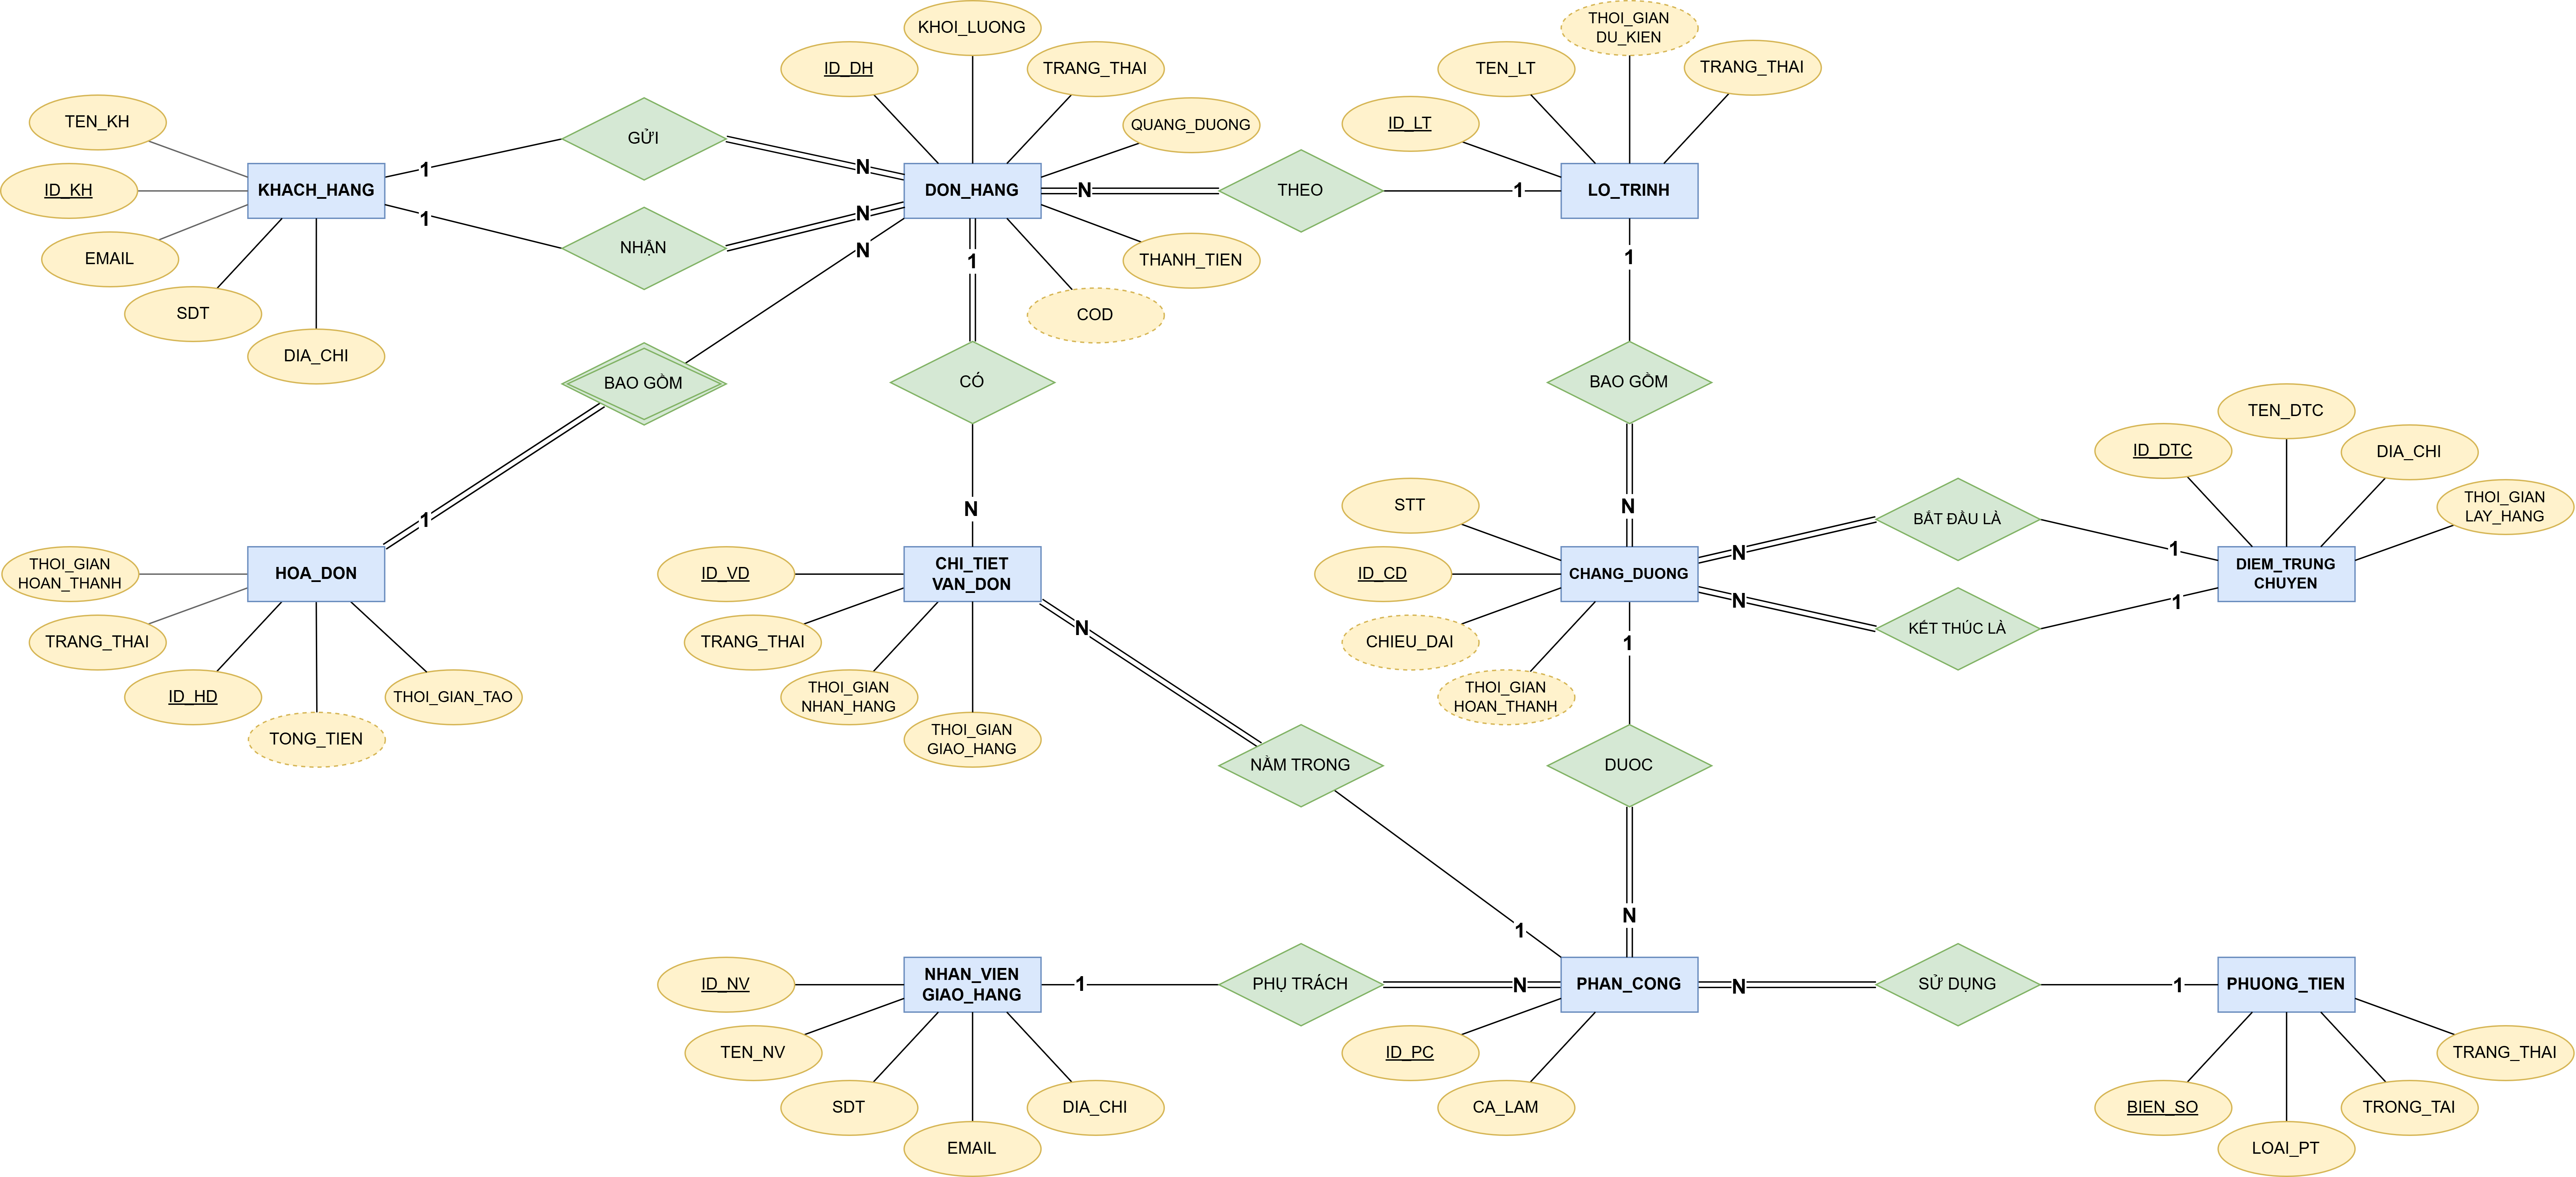
\includegraphics[width=0.95\textheight]{erd.png}}
    
    \caption{Sơ đồ thực thể liên kết}
    \label{fig:erd}
\end{figure}

% ========================================================================================================
% CHƯƠNG 4: THIẾT KẾ CƠ SỞ DỮ LIỆU QUAN HỆ
% ========================================================================================================

\chapter{Thiết kế cơ sở dữ liệu quan hệ}
\label{chap:thietke}

Chương này trình bày toàn bộ quá trình chuyển đổi mô hình ERD (Chương~\ref{chap:erd}) sang mô hình cơ sở dữ liệu quan hệ, thực hiện qua ba giai đoạn: 
\begin{enumerate}
    \item Ánh xạ từ ERD sang lược đồ quan hệ sơ khởi,
    \item Chuẩn hóa theo lý thuyết phụ thuộc hàm,
    \item Trình bày bản thiết kế cuối cùng.
\end{enumerate}
Phương pháp ánh xạ tuân theo bộ quy tắc chuẩn được hệ thống hóa trong~\cite{elmasri2015fundamentals}, còn lý thuyết chuẩn hóa dựa trên nền tảng phụ thuộc hàm và dạng chuẩn được trình bày trong~\cite{ieee1989er}.

% ========================================================================================================

\section{Ánh xạ từ mô hình ERD sang mô hình quan hệ}
\label{sec:anhxa}

\subsection{Nguyên tắc ánh xạ}
\label{subsec:nguyen_tac_anhxa}

Quá trình ánh xạ áp dụng bộ 7 quy tắc theo~\cite{elmasri2015fundamentals}. Bảng~\ref{tab:quytac_anhxa} tóm tắt từng quy tắc và cách áp dụng vào hệ thống.

\begin{table}[H]
    \rowcolors{2}{teal!5}{white}
    \centering
    \renewcommand{\tabularxcolumn}[1]{m{#1}}
    \begin{tabularx}{\textwidth}{|>{\raggedright\arraybackslash}l|>{\raggedright\arraybackslash}X|>{\raggedright\arraybackslash}X|} \hline
        \rowcolor{teal!30}
        \textbf{Quy tắc} & \textbf{Nội dung} & \textbf{Áp dụng trong hệ thống} \\ \hline
        QT1 & Mỗi thực thể mạnh $\to$ một quan hệ độc lập; thuộc tính dẫn xuất \textbf{không} lưu trữ & 10 thực thể mạnh $\to$ 10 bảng; loại bỏ 5 thuộc tính dẫn xuất: \texttt{COD}, \texttt{TONG\_TIEN}, \texttt{THOI\_GIAN\_DU\_KIEN}, \texttt{CHIEU\_DAI}, \texttt{THOI\_GIAN\_HOAN\_THANH} \\ \hline
        QT2 & Thực thể yếu $\to$ quan hệ với khóa chính là tổ hợp (discriminator + FK chủ) & Không có thực thể yếu trong thiết kế. \texttt{CHANG\_DUONG} là thực thể mạnh với \texttt{ID\_CD} làm PK độc lập; \texttt{STT} là thuộc tính thứ tự tạo khóa dự tuyển \texttt{(ID\_LT, STT)}, không phải discriminator theo nghĩa thực thể yếu \\ \hline
        QT3 & Quan hệ 1:1 $\to$ FK ở phía tham gia toàn phần & Không có quan hệ 1:1 thuần túy \\ \hline
        QT4 & Quan hệ 1:N $\to$ FK đặt vào phía N, tham chiếu PK phía 1 & Áp dụng cho toàn bộ 12 quan hệ \\ \hline
        QT5 & Quan hệ N:M $\to$ tạo bảng giao (junction table) mới & Không có quan hệ N:M thuần túy \\ \hline
        QT6 & Thuộc tính đa trị $\to$ tách thành bảng riêng & Không có thuộc tính đa trị \\ \hline
        QT7 & Quan hệ nhiều ngôi $\to$ bảng mới với FK đến tất cả thực thể tham gia & Không có quan hệ nhiều ngôi \\ \hline
    \end{tabularx}
    \caption{Bộ quy tắc ánh xạ ERD sang mô hình quan hệ}
    \label{tab:quytac_anhxa}
\end{table}

\subsection{Kết quả ánh xạ các thực thể}
\label{subsec:anhxa_thucthe}

Áp dụng QT1, 10 thực thể mạnh được ánh xạ thành 10 quan hệ. Năm thuộc tính dẫn xuất bị loại bỏ khỏi lược đồ quan hệ vì chúng có thể được tính toán lại qua truy vấn:

\begin{itemize}
    \item \texttt{COD} của \texttt{DON\_HANG}: tính từ \texttt{KHOI\_LUONG} và \texttt{QUANG\_DUONG} theo bảng cước vận chuyển.
    \item \texttt{TONG\_TIEN} của \texttt{HOA\_DON}: tính bằng tổng \texttt{COD} và \texttt{THANH\_TIEN} của tất cả \texttt{DON\_HANG} thuộc hóa đơn đó.
    \item \texttt{THOI\_GIAN\_DU\_KIEN} của \texttt{LO\_TRINH}: tổng thời gian hoàn thành các \texttt{CHANG\_DUONG} thuộc lộ trình.
    \item \texttt{CHIEU\_DAI} của \texttt{CHANG\_DUONG}: tính từ tọa độ/địa chỉ của hai \texttt{DIEM\_TRUNG\_CHUYEN} đầu và cuối chặng.
    \item \texttt{THOI\_GIAN\_HOAN\_THANH} của \texttt{CHANG\_DUONG}: tính từ \texttt{CHIEU\_DAI} và vận tốc trung bình theo loại đường.
\end{itemize}

Ký hiệu: \texttt{ENTITY}(\underline{\texttt{\color{Emerald} PRIMARY\_KEY}}, \texttt{ATTRIBUTE})

\noindent\textbf{Lưu ý:} Lược đồ \texttt{CHANG\_DUONG} sau QT1 chỉ còn \texttt{(ID\_CD, STT)} do hai thuộc tính \texttt{CHIEU\_DAI} và \texttt{THOI\_GIAN\_HOAN\_THANH} là thuộc tính dẫn xuất và đã bị loại bỏ theo nguyên tắc trên.

\begin{enumerate}
    \item \texttt{KHACH\_HANG}(\underline{\texttt{\color{Emerald} ID\_KH}},\ \texttt{TEN\_KH},\ \texttt{EMAIL},\ \texttt{SDT},\ \texttt{DIA\_CHI})
    \item \texttt{DON\_HANG}(\underline{\texttt{\color{Emerald} ID\_DH}},\ \texttt{KHOI\_LUONG},\ \texttt{QUANG\_DUONG},\ \texttt{TRANG\_THAI},\ \texttt{THANH\_TIEN})
    \item \texttt{LO\_TRINH}(\underline{\texttt{\color{Emerald} ID\_LT}},\ \texttt{TEN\_LT},\ \texttt{TRANG\_THAI})
    \item \texttt{CHANG\_DUONG}(\underline{\texttt{\color{Emerald} ID\_CD}},\ \texttt{STT})
    \item \texttt{DIEM\_TRUNG\_CHUYEN}(\underline{\texttt{\color{Emerald} ID\_DTC}},\ \texttt{TEN\_DTC},\ \texttt{DIA\_CHI},\ \texttt{THOI\_GIAN\_LAY\_HANG})
    \item \texttt{PHUONG\_TIEN}(\underline{\texttt{\color{Emerald} BIEN\_SO}},\ \texttt{LOAI\_PT},\ \texttt{TRONG\_TAI},\ \texttt{TRANG\_THAI})
    \item \texttt{NHAN\_VIEN\_GIAO\_HANG}(\underline{\texttt{\color{Emerald} ID\_NV}},\ \texttt{TEN\_NV},\ \texttt{SDT},\ \texttt{EMAIL},\ \texttt{DIA\_CHI})
    \item \texttt{PHAN\_CONG}(\underline{\texttt{\color{Emerald} ID\_PC}},\ \texttt{CA\_LAM})
    \item \texttt{CHI\_TIET\_VAN\_DON}(\underline{\texttt{\color{Emerald} ID\_VD}},\ \texttt{TRANG\_THAI},\ \texttt{THOI\_GIAN\_NHAN\_HANG},\ \texttt{THOI\_GIAN\_GIAO\_HANG})
    \item \texttt{HOA\_DON}(\underline{\texttt{\color{Emerald} ID\_HD}},\ \texttt{THOI\_GIAN\_TAO},\ \texttt{THOI\_GIAN\_HOAN\_THANH},\ \texttt{TRANG\_THAI})
\end{enumerate}

\subsection{Kết quả ánh xạ các mối liên kết}
\label{subsec:anhxa_moilienket}

Áp dụng QT4 cho toàn bộ 12 mối quan hệ 1:N trong ERD, khóa ngoại (FK) được bổ sung vào phía N. Bảng~\ref{tab:anhxa_lienket} tổng hợp kết quả.

\begin{table}[H]
    \rowcolors{2}{teal!5}{white}
    \centering
    \renewcommand{\tabularxcolumn}[1]{m{#1}}
    \small
    \begin{tabularx}{\textwidth}{|l|l|X|} \hline
        \rowcolor{teal!30}
        \textbf{Mối liên kết} & \textbf{Bảng nhận FK} & \textbf{Khóa ngoại bổ sung} \\ \hline
        \texttt{GỬI} (KH 1:N ĐH)          & \texttt{DON\_HANG}           & \texttt{ID\_KH\_GUI} $\to$ \texttt{KHACH\_HANG.ID\_KH} \\ \hline
        \texttt{NHẬN} (KH 1:N ĐH)         & \texttt{DON\_HANG}           & \texttt{ID\_KH\_NHAN} $\to$ \texttt{KHACH\_HANG.ID\_KH} \\ \hline
        \texttt{ĐI THEO} (ĐH N:1 LT)      & \texttt{DON\_HANG}           & \texttt{ID\_LT} $\to$ \texttt{LO\_TRINH.ID\_LT} \\ \hline
        \texttt{BAO GỒM} (HĐ 1:N ĐH)      & \texttt{DON\_HANG}           & \texttt{ID\_HD} $\to$ \texttt{HOA\_DON.ID\_HD} \\ \hline
        \texttt{CÓ} (ĐH 1:N VĐ)           & \texttt{CHI\_TIET\_VAN\_DON} & \texttt{ID\_DH} $\to$ \texttt{DON\_HANG.ID\_DH} \\ \hline
        \texttt{BAO GỒM} (LT 1:N CĐ)      & \texttt{CHANG\_DUONG}        & \texttt{ID\_LT} $\to$ \texttt{LO\_TRINH.ID\_LT} \\ \hline
        \texttt{BẮT ĐẦU LÀ} (CĐ N:1 ĐTC)  & \texttt{CHANG\_DUONG}        & \texttt{ID\_DTC\_BD} $\to$ \texttt{DIEM\_TRUNG\_CHUYEN.ID\_DTC} \\ \hline
        \texttt{KẾT THÚC LÀ} (CĐ N:1 ĐTC) & \texttt{CHANG\_DUONG}        & \texttt{ID\_DTC\_KT} $\to$ \texttt{DIEM\_TRUNG\_CHUYEN.ID\_DTC} \\ \hline
        \texttt{ĐƯỢC} (CĐ 1:N PC)         & \texttt{PHAN\_CONG}          & \texttt{ID\_CD} $\to$ \texttt{CHANG\_DUONG.ID\_CD} \\ \hline
        \texttt{PHỤ TRÁCH} (NV 1:N PC)    & \texttt{PHAN\_CONG}          & \texttt{ID\_NV} $\to$ \texttt{NHAN\_VIEN\_GIAO\_HANG.ID\_NV} \\ \hline
        \texttt{SỬ DỤNG} (PC N:1 PT)      & \texttt{PHAN\_CONG}          & \texttt{BIEN\_SO} $\to$ \texttt{PHUONG\_TIEN.BIEN\_SO} \\ \hline
        \texttt{NẰM TRONG} (VĐ N:1 PC)    & \texttt{CHI\_TIET\_VAN\_DON} & \texttt{ID\_PC} $\to$ \texttt{PHAN\_CONG.ID\_PC} \\ \hline
    \end{tabularx}
    \caption{Kết quả ánh xạ các mối liên kết sang khóa ngoại}
    \label{tab:anhxa_lienket}
\end{table}

\noindent\textbf{Lưu ý:} \texttt{DON\_HANG.ID\_HD} cho phép \texttt{NULL} vì hóa đơn chỉ được tạo sau khi toàn bộ chi tiết vận đơn đạt trạng thái \texttt{'Da giao'} --- đơn hàng mới tiếp nhận chưa có hóa đơn. 

Ký hiệu: \texttt{ENTITY}(\boxed{\texttt{\color{Emerald} PRIMARY\_KEY}}, \texttt{ATTRIBUTE}, \underline{\texttt{\color{RoyalBlue} FOREIGN\_KEY}})

Lược đồ quan hệ đầy đủ sau khi bổ sung khóa ngoại:

\begin{enumerate}
    \item \texttt{KHACH\_HANG}(\boxed{\texttt{\color{Emerald} ID\_KH}},\ \texttt{TEN\_KH},\ \texttt{EMAIL},\ \texttt{SDT},\ \texttt{DIA\_CHI})
    \item \texttt{DON\_HANG}(\boxed{\texttt{\color{Emerald} ID\_DH}},\ \texttt{KHOI\_LUONG},\ \texttt{QUANG\_DUONG},\ \texttt{TRANG\_THAI},\ \texttt{THANH\_TIEN},\ \underline{\texttt{\color{RoyalBlue}ID\_KH\_GUI}},\\
          \underline{\texttt{\color{RoyalBlue}ID\_KH\_NHAN}},\ \underline{\texttt{\color{RoyalBlue}ID\_LT}},\ \underline{\texttt{\color{RoyalBlue}ID\_HD}})
    \item \texttt{LO\_TRINH}(\boxed{\texttt{\color{Emerald} ID\_LT}},\ \texttt{TEN\_LT},\ \texttt{TRANG\_THAI})
    \item \texttt{CHANG\_DUONG}(\boxed{\texttt{\color{Emerald} ID\_CD}},\ \texttt{STT},\ \underline{\texttt{\color{RoyalBlue}ID\_LT}},\ \underline{\texttt{\color{RoyalBlue}ID\_DTC\_BD}},\ \underline{\texttt{\color{RoyalBlue}ID\_DTC\_KT}})
    \item \texttt{DIEM\_TRUNG\_CHUYEN}(\boxed{\texttt{\color{Emerald} ID\_DTC}},\ \texttt{TEN\_DTC},\ \texttt{DIA\_CHI},\ \texttt{THOI\_GIAN\_LAY\_HANG})
    \item \texttt{PHUONG\_TIEN}(\boxed{\texttt{\color{Emerald} BIEN\_SO}},\ \texttt{LOAI\_PT},\ \texttt{TRONG\_TAI},\ \texttt{TRANG\_THAI})
    \item \texttt{NHAN\_VIEN\_GIAO\_HANG}(\boxed{\texttt{\color{Emerald} ID\_NV}},\ \texttt{TEN\_NV},\ \texttt{SDT},\ \texttt{EMAIL},\ \texttt{DIA\_CHI})
    \item \texttt{PHAN\_CONG}(\boxed{\texttt{\color{Emerald} ID\_PC}},\ \texttt{CA\_LAM},\ \underline{\texttt{\color{RoyalBlue}ID\_CD}},\ \underline{\texttt{\color{RoyalBlue}ID\_NV}},\ \underline{\texttt{\color{RoyalBlue}BIEN\_SO}})
    \item \texttt{CHI\_TIET\_VAN\_DON}(\boxed{\texttt{\color{Emerald} ID\_VD}},\ \texttt{TRANG\_THAI},\ \texttt{THOI\_GIAN\_NHAN\_HANG},\ \texttt{THOI\_GIAN\_GIAO\_HANG},\ \underline{\texttt{\color{RoyalBlue}ID\_DH}},\ \underline{\texttt{\color{RoyalBlue}ID\_PC}})
    \item \texttt{HOA\_DON}(\boxed{\texttt{\color{Emerald} ID\_HD}},\ \texttt{THOI\_GIAN\_TAO},\ \texttt{THOI\_GIAN\_HOAN\_THANH},\ \texttt{TRANG\_THAI})
\end{enumerate}

% ========================================================================================================

\section{Chuẩn hóa lược đồ quan hệ}
\label{sec:chuanhoa}

\subsection{Liệt kê các phụ thuộc hàm}
\label{subsec:pth}

Phụ thuộc hàm (Functional Dependency --- FD) X $\rightarrow$ Y biểu diễn mối quan hệ: Với mọi hai bộ dữ liệu có cùng giá trị trên tập thuộc tính X, chúng cũng phải có cùng giá trị trên tập thuộc tính Y~\cite{elmasri2015fundamentals}. Dưới đây liệt kê đầy đủ các phụ thuộc hàm không tầm thường của từng lược đồ:

\begin{enumerate}
    \item \texttt{KHACH\_HANG}: \texttt{ID\_KH} \rightarrow \ \texttt{TEN\_KH},\ \texttt{EMAIL},\ \texttt{SDT},\ \texttt{DIA\_CHI}

    \item \texttt{DON\_HANG}: \texttt{ID\_DH} \rightarrow \ \texttt{KHOI\_LUONG},\ \texttt{QUANG\_DUONG},\ \texttt{TRANG\_THAI},\ \texttt{THANH\_TIEN},\ \texttt{ID\_KH\_GUI},\\ 
          \texttt{ID\_KH\_NHAN},\ \texttt{ID\_LT},\ \texttt{ID\_HD}

    \item \texttt{LO\_TRINH}: \texttt{ID\_LT} \rightarrow \ \texttt{TEN\_LT},\ \texttt{TRANG\_THAI}

    \item\texttt{CHANG\_DUONG}: \hfill
        \begin{itemize}
            \item \texttt{ID\_CD} \rightarrow \ \texttt{STT},\ \texttt{ID\_LT},\ \texttt{ID\_DTC\_BD},\ \texttt{ID\_DTC\_KT}
            
            \item (\texttt{ID\_LT},\ \texttt{STT}) \rightarrow \ \texttt{ID\_CD},\ \texttt{ID\_DTC\_BD},\ \texttt{ID\_DTC\_KT}
        \end{itemize}

    \item \texttt{DIEM\_TRUNG\_CHUYEN}: \texttt{ID\_DTC} \rightarrow \ \texttt{TEN\_DTC},\ \texttt{DIA\_CHI},\ \texttt{THOI\_GIAN\_LAY\_HANG}

    \item \texttt{PHUONG\_TIEN}: \texttt{BIEN\_SO} \rightarrow \ \texttt{LOAI\_PT},\ \texttt{TRONG\_TAI},\ \texttt{TRANG\_THAI}

    \item \texttt{NHAN\_VIEN\_GIAO\_HANG}: \texttt{ID\_NV} \rightarrow \ \texttt{TEN\_NV},\ \texttt{SDT},\ \texttt{EMAIL},\ \texttt{DIA\_CHI}

    \item \texttt{PHAN\_CONG}: \texttt{ID\_PC} \rightarrow \ \texttt{CA\_LAM},\ \texttt{ID\_CD},\ \texttt{ID\_NV},\ \texttt{BIEN\_SO}

    \item\texttt{CHI\_TIET\_VAN\_DON}: \hfill
        \begin{itemize}
            \item \texttt{ID\_VD} \rightarrow \ \texttt{TRANG\_THAI},\ \texttt{THOI\_GIAN\_NHAN\_HANG},\ \texttt{THOI\_GIAN\_GIAO\_HANG},\ \texttt{ID\_DH},\ \texttt{ID\_PC}
            
            \item (\texttt{ID\_DH}, \texttt{ID\_PC})\rightarrow \texttt{ID\_VD}, \texttt{TRANG\_THAI}, \texttt{THOI\_GIAN\_NHAN\_HANG}, \texttt{THOI\_GIAN\_GIAO\_HANG}
        \end{itemize}

    \item\texttt{HOA\_DON}:
        \texttt{ID\_HD} \rightarrow \ \texttt{THOI\_GIAN\_TAO},\ \texttt{THOI\_GIAN\_HOAN\_THANH},\ \texttt{TRANG\_THAI}
\end{enumerate}

\textbf{Nhận xét:} Hai lược đồ có nhiều hơn một khóa dự tuyển (candidate key) là:
\begin{itemize}
    \item \texttt{CHANG\_DUONG} --- CK1: \texttt{ID\_CD}; CK2: \texttt{(ID\_LT, STT)},
    
    \item \texttt{CHI\_TIET\_VAN\_DON} --- CK1: \texttt{ID\_VD}; CK2: \texttt{(ID\_DH, ID\_PC)}.
\end{itemize}  
Đây là hai trường hợp cần kiểm tra kỹ lưỡng trong phân tích dạng chuẩn.

\subsection{Xác định khóa của các lược đồ quan hệ}
\label{subsec:xacdinhkhoa}

Bảng~\ref{tab:fkvack} tổng hợp khóa chính (PK) và các khóa dự tuyển (CK) của từng lược đồ.

\begin{table}[H]
    \rowcolors{2}{teal!5}{white}
    \centering
    \renewcommand{\tabularxcolumn}[1]{m{#1}}
    \begin{tabularx}{\textwidth}{|l|l|X|} \hline
        \rowcolor{teal!30}
        \textbf{Lược đồ} & \textbf{Khóa chính (PK)} & \textbf{Khóa dự tuyển khác (CK)} \\ \hline
        \texttt{KHACH\_HANG}            & \texttt{ID\_KH}   & \texttt{EMAIL} (đã khai báo \texttt{UNIQUE} trong thiết kế) \\ \hline
        \texttt{DON\_HANG}              & \texttt{ID\_DH}   & --- \\ \hline
        \texttt{LO\_TRINH}              & \texttt{ID\_LT}   & --- \\ \hline
        \texttt{CHANG\_DUONG}           & \texttt{ID\_CD}   & \texttt{(ID\_LT, STT)} \\ \hline
        \texttt{DIEM\_TRUNG\_CHUYEN}    & \texttt{ID\_DTC}  & --- \\ \hline
        \texttt{PHUONG\_TIEN}           & \texttt{BIEN\_SO} & --- \\ \hline
        \texttt{NHAN\_VIEN\_GIAO\_HANG} & \texttt{ID\_NV}   & \texttt{SDT}, \texttt{EMAIL} (đã khai báo \texttt{UNIQUE} trong thiết kế) \\ \hline
        \texttt{PHAN\_CONG}             & \texttt{ID\_PC}   & --- \\ \hline
        \texttt{CHI\_TIET\_VAN\_DON}    & \texttt{ID\_VD}   & \texttt{(ID\_DH, ID\_PC)} \\ \hline
        \texttt{HOA\_DON}               & \texttt{ID\_HD}   & --- \\ \hline
    \end{tabularx}
    \caption{Khóa chính và khóa dự tuyển của các lược đồ quan hệ}
    \label{tab:fkvack}
\end{table}

\subsection{Kiểm tra dạng chuẩn}
\label{subsec:kiemtra_dang_chuan}

\subsubsection{Kiểm tra dạng chuẩn 1 (1NF)}

Một lược đồ quan hệ đạt \textbf{1NF} khi và chỉ khi miền giá trị của mọi thuộc tính là nguyên tử (atomic) --- không phân chia được, không có giá trị tập hợp hay nhóm lặp~\cite{elmasri2015fundamentals}.

\noindent Kiểm tra toàn bộ 10 lược đồ:
\begin{itemize}
    \item Tất cả thuộc tính đều đơn trị và nguyên tử: \texttt{TEN\_KH}, \texttt{TRANG\_THAI},~\ldots là chuỗi ký tự đơn; \texttt{KHOI\_LUONG}, \texttt{TRONG\_TAI} là số thực; \texttt{THOI\_GIAN\_*} là giá trị thời điểm đơn; \texttt{STT} là số nguyên.
    
    \item Không có thuộc tính đa trị (đã tách thành thực thể riêng trong giai đoạn ER).
    
    \item Không có nhóm lặp (repeating groups).
\end{itemize}
$\Rightarrow$ \textbf{Tất cả 10 lược đồ đều đạt 1NF.}

\subsubsection{Kiểm tra dạng chuẩn 2 (2NF)}

Một lược đồ đạt \textbf{2NF} khi đạt 1NF và mọi thuộc tính không nguyên tố (non-prime attribute) đều \textbf{phụ thuộc hàm đầy đủ} vào mọi khóa dự tuyển --- không tồn tại phụ thuộc bộ phận (partial dependency)~\cite{elmasri2015fundamentals}.

Các lược đồ có PK đơn thuộc tính (\texttt{KHACH\_HANG}, \texttt{DON\_HANG}, \texttt{LO\_TRINH}, \texttt{DIEM\_TRUNG\_CHUYEN}, \texttt{PHUONG\_TIEN}, \texttt{NHAN\_VIEN\_GIAO\_HANG}, \texttt{PHAN\_CONG}, \texttt{HOA\_DON}): không thể có phụ thuộc bộ phận với PK đơn thuộc tính $\Rightarrow$ Tự động đạt 2NF.

Hai lược đồ cần kiểm tra kỹ với CK tổ hợp:

\begin{itemize}
    \item \texttt{CHANG\_DUONG} với CK2 = \texttt{(ID\_LT, STT)}. Các thuộc tính không nguyên tố (theo CK2): \texttt{ID\_CD}, \texttt{ID\_DTC\_BD}, \texttt{ID\_DTC\_KT}.
    \begin{itemize}
        \item \texttt{ID\_DTC\_BD}: điểm bắt đầu là đặc trưng của từng chặng cụ thể, không xác định được chỉ từ \texttt{ID\_LT} (vì lộ trình có nhiều chặng) hay chỉ từ \texttt{STT} (vì STT không xác định duy nhất chặng) $\Rightarrow$ Phụ thuộc đầy đủ vào \texttt{(ID\_LT, STT)}.
        
        \item \texttt{ID\_DTC\_KT}, \texttt{ID\_CD}: lập luận tương tự $\Rightarrow$ Phụ thuộc đầy đủ.
    \end{itemize}
    $\Rightarrow$ \texttt{CHANG\_DUONG} đạt 2NF.

    \item \texttt{CHI\_TIET\_VAN\_DON} với CK2 = \texttt{(ID\_DH, ID\_PC)}. Các thuộc tính không nguyên tố (theo CK2): \texttt{ID\_VD}, \texttt{TRANG\_THAI}, \texttt{THOI\_GIAN\_NHAN\_HANG}, \texttt{THOI\_GIAN\_GIAO\_HANG}.
    \begin{itemize}
        \item \texttt{TRANG\_THAI}: là trạng thái của đơn hàng trên một phân công cụ thể, không xác định được chỉ từ \texttt{ID\_DH} (vì một đơn hàng có nhiều chi tiết vận đơn) hay chỉ từ \texttt{ID\_PC} (vì một phân công chở nhiều đơn hàng) $\Rightarrow$ Phụ thuộc đầy đủ.
        
        \item \texttt{THOI\_GIAN\_NHAN\_HANG}, \texttt{THOI\_GIAN\_GIAO\_HANG}, \texttt{ID\_VD}: lập luận tương tự $\Rightarrow$ Phụ thuộc đầy đủ.
    \end{itemize}
    $\Rightarrow$ \texttt{CHI\_TIET\_VAN\_DON} đạt 2NF.
\end{itemize}
$\Rightarrow$ \textbf{Tất cả 10 lược đồ đều đạt 2NF.}

\subsubsection{Kiểm tra dạng chuẩn 3 (3NF)}

Một lược đồ đạt \textbf{3NF} khi đạt 2NF và không tồn tại \textbf{phụ thuộc bắc cầu} (transitive dependency): không có thuộc tính không nguyên tố Z nào mà \texttt{KEY} $\to$ X $\to$ Z với X không là siêu khóa~\cite{elmasri2015fundamentals}.

Kiểm tra các lược đồ có khóa ngoại (nơi phụ thuộc bắc cầu tiềm ẩn phổ biến nhất):
\begin{itemize}
    \item \texttt{DON\_HANG}: \texttt{ID\_DH} $\to$ \texttt{ID\_LT}, và từ \texttt{LO\_TRINH}: \texttt{ID\_LT} $\to$ \texttt{TEN\_LT}. Tuy nhiên \texttt{TEN\_LT} không thuộc lược đồ \texttt{DON\_HANG} $\Rightarrow$ Không có phụ thuộc bắc cầu nội bộ.
    
    \item \texttt{DON\_HANG}: \texttt{ID\_DH} $\to$ \texttt{ID\_KH\_GUI}, và \texttt{ID\_KH\_GUI} $\to$ \texttt{TEN\_KH}. Tuy nhiên \texttt{TEN\_KH} không thuộc \texttt{DON\_HANG} $\Rightarrow$ Không vi phạm 3NF.
    
    \item \texttt{PHAN\_CONG}: \texttt{ID\_PC} $\to$ \texttt{ID\_CD}, và \texttt{ID\_CD} $\to$ \texttt{STT},~\ldots, nhưng \texttt{STT} không thuộc \texttt{PHAN\_CONG} $\Rightarrow$ Không vi phạm 3NF.
    
    \item Các lược đồ còn lại: các FK chỉ là con trỏ sang bảng khác, không kéo thuộc tính mô tả từ bảng đó vào $\Rightarrow$ Không có phụ thuộc bắc cầu.
\end{itemize}
$\Rightarrow$ \textbf{Tất cả 10 lược đồ đều đạt 3NF.}

\subsubsection{Kiểm tra dạng chuẩn Boyce-Codd (BCNF)}

Một lược đồ đạt \textbf{BCNF} khi với mọi phụ thuộc hàm không tầm thường X $\to$ Y, X phải là \textbf{siêu khóa} (superkey)~\cite{ieee1989er}. BCNF chặt hơn 3NF và chỉ khác 3NF ở các lược đồ có nhiều khóa dự tuyển giao nhau.

Kiểm tra hai lược đồ có nhiều CK:
\begin{itemize}
    \item \texttt{CHANG\_DUONG}: Toàn bộ phụ thuộc hàm (FD) không tầm thường:
    \begin{itemize}
        \item $\texttt{ID\_CD} \to \{\texttt{STT},\ \texttt{ID\_LT},\ \texttt{ID\_DTC\_BD},\ \texttt{ID\_DTC\_KT}\}$: \texttt{ID\_CD} là CK1 $\Rightarrow$ Siêu khóa. 
        
        \item $(\texttt{ID\_LT},\ \texttt{STT}) \to \{\texttt{ID\_CD},\ \texttt{ID\_DTC\_BD},\ \texttt{ID\_DTC\_KT}\}$: \texttt{(ID\_LT, STT)} là CK2 $\Rightarrow$ Siêu khóa. 
        
        \item Không tồn tại phụ thuộc hàm (FD) nào có vế trái không là siêu khóa.
    \end{itemize}
    $\Rightarrow$ \texttt{CHANG\_DUONG} đạt BCNF.

    \item \texttt{CHI\_TIET\_VAN\_DON}: Toàn bộ phụ thuộc hàm (FD) không tầm thường:
    \begin{itemize}
        \item $\texttt{ID\_VD} \to \{\ldots\}$: \texttt{ID\_VD} là CK1 $\Rightarrow$ Siêu khóa. 
        
        \item $(\texttt{ID\_DH},\ \texttt{ID\_PC}) \to \{\ldots\}$: \texttt{(ID\_DH, ID\_PC)} là CK2 $\Rightarrow$ Siêu khóa. 
    \end{itemize}
    $\Rightarrow$ \texttt{CHI\_TIET\_VAN\_DON} đạt BCNF.

    \item 8 lược đồ còn lại có duy nhất một CK $\Rightarrow$ với lược đồ một CK, 3NF $\equiv$ BCNF $\Rightarrow$ Đều đạt BCNF.
\end{itemize}

$\Rightarrow$ \textbf{Tất cả 10 lược đồ đều đạt BCNF.}

\subsection{Chuẩn hóa về dạng chuẩn cao hơn}
\label{subsec:dang_chuan_cao_hon}

\textbf{Dạng chuẩn 4 (4NF)} yêu cầu không tồn tại phụ thuộc đa trị (Multi-Valued Dependency --- MVD) không tầm thường nào mà vế trái không là siêu khóa~\cite{elmasri2015fundamentals}. Phụ thuộc đa trị X $\twoheadrightarrow$ Y xuất hiện khi một giá trị X xác định một tập hợp giá trị Y độc lập với các thuộc tính còn lại của quan hệ.

Kiểm tra: Trong thiết kế hiện tại, không có lược đồ nào chứa hai thuộc tính đa trị độc lập nhau cùng phụ thuộc vào một khóa. Mọi thực thể có thuộc tính đa trị tiềm năng (tập chặng đường của lộ trình, tập chi tiết vận đơn của đơn hàng) đều đã được tách thành bảng riêng trong giai đoạn thiết kế ERD.

\textbf{Phân tích trường hợp đặc thù --- bảng \texttt{PHAN\_CONG}:} Bảng \texttt{PHAN\_CONG(\underline{ID\_PC}, CA\_LAM, ID\_CD, ID\_NV, BIEN\_SO)} là lược đồ có khả năng phát sinh MVD cao nhất trong thiết kế, do liên kết ba thực thể \texttt{CHANG\_DUONG}, \texttt{NHAN\_VIEN\_GIAO\_HANG} và \texttt{PHUONG\_TIEN}. Câu hỏi đặt ra: liệu có tồn tại \texttt{ID\_NV} $\twoheadrightarrow$ \texttt{BIEN\_SO} không? Tức là, với một nhân viên cố định, tập xe họ sử dụng có độc lập với chặng đường họ đang chạy không?

Câu trả lời là \textbf{không}: mỗi bản ghi trong \texttt{PHAN\_CONG} biểu diễn một \textit{sự kiện vận hành cụ thể} --- nhân viên $X$ lái xe $Y$ chạy chặng $Z$ trong ca $W$. Sự kết hợp \texttt{(ID\_NV, BIEN\_SO, ID\_CD, CA\_LAM)} là một quyết định điều phối đơn lẻ, không tách rời. Một nhân viên không tự do chọn xe bất kỳ cho mỗi chặng; việc phân công xe gắn liền với chặng cụ thể được giao. Do đó, \texttt{ID\_NV $\twoheadrightarrow$ BIEN\_SO} \textbf{không tồn tại} trong ngữ nghĩa nghiệp vụ này.

Do đó, không tồn tại MVD không tầm thường nào vi phạm 4NF trên toàn bộ 10 lược đồ.

$\Rightarrow$ \textbf{Tất cả 10 lược đồ đều đạt 4NF. Không cần chuẩn hóa thêm.}

\section{Bản thiết kế cơ sở dữ liệu cuối cùng}
\label{sec:thietke_cuoi}

Kết quả chuẩn hóa xác nhận toàn bộ 10 lược đồ quan hệ đã đạt BCNF và 4NF ngay sau bước ánh xạ. Phần này mô tả chi tiết cấu trúc các bảng và ràng buộc dữ liệu phục vụ triển khai trên SQL Server. Quy ước ký hiệu: \textbf{PK} = khóa chính, \textbf{FK} = khóa ngoại.

\subsection{Mô tả cấu trúc các bảng}
\label{subsec:cau_truc_bang}

\noindent\textbf{Bảng \texttt{KHACH\_HANG}} --- Lưu thông tin khách hàng (người gửi và người nhận).
\begin{table}[H]
    \rowcolors{2}{teal!5}{white}
    \centering
    \renewcommand{\tabularxcolumn}[1]{m{#1}}
    \begin{tabularx}{\textwidth}{|l|l|l|X|} \hline
        \rowcolor{teal!30}
        \textbf{Tên cột} & \textbf{Kiểu dữ liệu} & \textbf{Ràng buộc} & \textbf{Mô tả} \\ \hline
        \texttt{ID\_KH}   & \texttt{VARCHAR(10)}   & \texttt{PK, NOT NULL}  & Mã khách hàng \\ \hline
        \texttt{TEN\_KH}  & \texttt{NVARCHAR(100)} & \texttt{NOT NULL}      & Họ và tên đầy đủ \\ \hline
        \texttt{EMAIL}    & \texttt{VARCHAR(100)}  & \texttt{UNIQUE}  & Địa chỉ email \\ \hline
        \texttt{SDT}      & \texttt{VARCHAR(15)}   & \texttt{NOT NULL}      & Số điện thoại \\ \hline
        \texttt{DIA\_CHI} & \texttt{NVARCHAR(200)} & \texttt{NOT NULL}      & Địa chỉ liên hệ \\ \hline
    \end{tabularx}
    \caption{Cấu trúc bảng \texttt{KHACH\_HANG}}
    \label{tab:str_khachhang}
\end{table}

\noindent\textbf{Bảng HOA\_DON} --- Lưu chứng từ tài chính (khai báo trước \texttt{DON\_HANG} vì có FK trỏ sang; \texttt{TONG\_TIEN} là thuộc tính dẫn xuất, không lưu trữ).
\begin{table}[H]
    \rowcolors{2}{teal!5}{white}
    \centering
    \renewcommand{\tabularxcolumn}[1]{m{#1}}
    \begin{tabularx}{\textwidth}{|l|l|l|>{\raggedright\arraybackslash}X|} \hline
        \rowcolor{teal!30}
        \textbf{Tên cột} & \textbf{Kiểu dữ liệu} & \textbf{Ràng buộc} & \textbf{Mô tả} \\ \hline
        \texttt{ID\_HD}                  & \texttt{VARCHAR(10)}  & \texttt{PK, NOT NULL}  & Mã hóa đơn \\ \hline
        \texttt{THOI\_GIAN\_TAO}         & \texttt{DATETIME}     & \texttt{NOT NULL}      & Thời điểm tạo hóa đơn \\ \hline
        \texttt{THOI\_GIAN\_HOAN\_THANH} & \texttt{DATETIME}     & \texttt{NULL}          & Thời điểm thanh toán (\texttt{NULL} nếu chưa thanh) \\ \hline
        \texttt{TRANG\_THAI}             & \texttt{NVARCHAR(50)} & \texttt{NOT NULL}      & \texttt{'Chua thanh toan'} / \texttt{'Da thanh toan'} \\ \hline
    \end{tabularx}
    \caption{Cấu trúc bảng \texttt{HOA\_DON}}
    \label{tab:str_hoadon}
\end{table}

\noindent\textbf{Bảng \texttt{LO\_TRINH}} --- Lưu thông tin các tuyến vận chuyển (\texttt{THOI\_GIAN\_DU\_KIEN} là thuộc tính dẫn xuất, tính bằng tổng thời gian các chặng, không lưu trữ).
\begin{table}[H]
    \rowcolors{2}{teal!5}{white}
    \centering
    \renewcommand{\tabularxcolumn}[1]{m{#1}}
    \begin{tabularx}{\textwidth}{|l|l|l|X|} \hline
        \rowcolor{teal!30}
        \textbf{Tên cột} & \textbf{Kiểu dữ liệu} & \textbf{Ràng buộc} & \textbf{Mô tả} \\ \hline
        \texttt{ID\_LT}      & \texttt{VARCHAR(10)}   & \texttt{PK, NOT NULL}  & Mã lộ trình \\ \hline
        \texttt{TEN\_LT}     & \texttt{NVARCHAR(200)} & \texttt{NOT NULL}      & Tên mô tả tuyến đường \\ \hline
        \texttt{TRANG\_THAI} & \texttt{NVARCHAR(50)}  & \texttt{NOT NULL}      & \texttt{'Dang hoat dong'} / \texttt{'Tam dung'} \\ \hline
    \end{tabularx}
    \caption{Cấu trúc bảng \texttt{LO\_TRINH}}
    \label{tab:str_lotrinh}
\end{table}

\noindent\textbf{Bảng \texttt{DON\_HANG}} --- Lưu thông tin đơn hàng vận chuyển (\texttt{COD} là thuộc tính dẫn xuất, tính từ \texttt{KHOI\_LUONG} và \texttt{QUANG\_DUONG}, không lưu trữ).
\begin{table}[H]
    \rowcolors{2}{teal!5}{white}
    \centering
    \renewcommand{\tabularxcolumn}[1]{m{#1}}
    \begin{tabularx}{\textwidth}{|l|l|l|>{\raggedright\arraybackslash}X|} \hline
        \rowcolor{teal!30}
        \textbf{Tên cột} & \textbf{Kiểu dữ liệu} & \textbf{Ràng buộc} & \textbf{Mô tả} \\ \hline
        \texttt{ID\_DH}       & \texttt{VARCHAR(10)}   & \texttt{PK, NOT NULL}   & Mã đơn hàng \\ \hline
        \texttt{KHOI\_LUONG}  & \texttt{DECIMAL(10,2)} & \texttt{NOT NULL}       & Khối lượng hàng (kg) \\ \hline
        \texttt{QUANG\_DUONG} & \texttt{DECIMAL(10,2)} & \texttt{NOT NULL}       & Tổng quãng đường (km) \\ \hline
        \texttt{TRANG\_THAI}  & \texttt{NVARCHAR(50)}  & \texttt{NOT NULL}       & \texttt{'Cho xu ly'} / \texttt{'Dang van chuyen'} / \texttt{'Da giao'} / \texttt{'Hoan tra'} \\ \hline
        \texttt{THANH\_TIEN}  & \texttt{DECIMAL(15,2)} & \texttt{NOT NULL}       & Giá trị hàng hóa khai báo (VNĐ) \\ \hline
        \texttt{ID\_KH\_GUI}  & \texttt{VARCHAR(10)}   & \texttt{FK, NOT NULL}   & Khách hàng gửi hàng \\ \hline
        \texttt{ID\_KH\_NHAN} & \texttt{VARCHAR(10)}   & \texttt{FK, NOT NULL}   & Khách hàng nhận hàng \\ \hline
        \texttt{ID\_LT}       & \texttt{VARCHAR(10)}   & \texttt{FK, NOT NULL}   & Lộ trình vận chuyển \\ \hline
        \texttt{ID\_HD}       & \texttt{VARCHAR(10)}   & \texttt{FK, NULL} & Hóa đơn thanh toán (\texttt{NULL} khi chưa xuất hóa đơn) \\ \hline
    \end{tabularx}
    \caption{Cấu trúc bảng \texttt{DON\_HANG}}
    \label{tab:str_donhang}
\end{table}

\noindent\textbf{Bảng \texttt{DIEM\_TRUNG\_CHUYEN}} --- Lưu thông tin các điểm trung chuyển.
\begin{table}[H]
    \rowcolors{2}{teal!5}{white}
    \centering
    \renewcommand{\tabularxcolumn}[1]{m{#1}}
    \begin{tabularx}{\textwidth}{|l|l|l|X|} \hline
        \rowcolor{teal!30}
        \textbf{Tên cột} & \textbf{Kiểu dữ liệu} & \textbf{Ràng buộc} & \textbf{Mô tả} \\ \hline
        \texttt{ID\_DTC}               & \texttt{VARCHAR(10)}   & \texttt{PK, NOT NULL}  & Mã điểm trung chuyển \\ \hline
        \texttt{TEN\_DTC}              & \texttt{NVARCHAR(100)} & \texttt{NOT NULL}      & Tên điểm trung chuyển \\ \hline
        \texttt{DIA\_CHI}              & \texttt{NVARCHAR(200)} & \texttt{NOT NULL}      & Địa chỉ vật lý \\ \hline
        \texttt{THOI\_GIAN\_LAY\_HANG} & \texttt{NVARCHAR(50)}  & \texttt{NULL}          & Khung giờ nhận hàng \\ \hline
    \end{tabularx}
    \caption{Cấu trúc bảng \texttt{DIEM\_TRUNG\_CHUYEN}}
    \label{tab:str_dtc}
\end{table}

\noindent\textbf{Bảng \texttt{CHANG\_DUONG}} --- Lưu thông tin của chặng đường đi qua trong lộ trình (\texttt{CHIEU\_DAI} và \texttt{THOI\_GIAN\_HOAN\_THANH} là thuộc tính dẫn xuất, không lưu trữ).
\begin{table}[H]
    \rowcolors{2}{teal!5}{white}
    \centering
    \renewcommand{\tabularxcolumn}[1]{m{#1}}
    \begin{tabularx}{\textwidth}{|l|l|l|X|} \hline
        \rowcolor{teal!30}
        \textbf{Tên cột} & \textbf{Kiểu dữ liệu} & \textbf{Ràng buộc} & \textbf{Mô tả} \\ \hline
        \texttt{ID\_CD}      & \texttt{VARCHAR(10)} & \texttt{PK, NOT NULL}  & Mã chặng đường \\ \hline
        \texttt{STT}         & \texttt{INT}         & \texttt{NOT NULL}      & Số thứ tự trong lộ trình \\ \hline
        \texttt{ID\_LT}      & \texttt{VARCHAR(10)} & \texttt{FK, NOT NULL}  & Lộ trình chứa chặng này \\ \hline
        \texttt{ID\_DTC\_BD} & \texttt{VARCHAR(10)} & \texttt{FK, NOT NULL}  & Điểm trung chuyển bắt đầu \\ \hline
        \texttt{ID\_DTC\_KT} & \texttt{VARCHAR(10)} & \texttt{FK, NOT NULL}  & Điểm trung chuyển kết thúc \\ \hline
    \end{tabularx}
    \caption{Cấu trúc bảng \texttt{CHANG\_DUONG}}
    \label{tab:str_changduong}
\end{table}

\noindent\textbf{Bảng \texttt{PHUONG\_TIEN}} --- Lưu thông tin phương tiện vận chuyển.
\begin{table}[H]
    \rowcolors{2}{teal!5}{white}
    \centering
    \renewcommand{\tabularxcolumn}[1]{m{#1}}
    \begin{tabularx}{\textwidth}{|l|l|l|X|} \hline
        \rowcolor{teal!30}
        \textbf{Tên cột} & \textbf{Kiểu dữ liệu} & \textbf{Ràng buộc} & \textbf{Mô tả} \\ \hline
        \texttt{BIEN\_SO}    & \texttt{VARCHAR(15)}   & \texttt{PK, NOT NULL}  & Biển số đăng ký \\ \hline
        \texttt{LOAI\_PT}    & \texttt{NVARCHAR(50)}  & \texttt{NOT NULL}      & Loại phương tiện (\texttt{'Xe may'}, \texttt{'Xe tai'}, \texttt{'Xe container'}) \\ \hline
        \texttt{TRONG\_TAI}  & \texttt{DECIMAL(10,2)} & \texttt{NOT NULL}      & Trọng tải tối đa (kg) \\ \hline
        \texttt{TRANG\_THAI} & \texttt{NVARCHAR(50)}  & \texttt{NOT NULL}      & \texttt{'Hoat dong'} / \texttt{'Bao tri'} \\ \hline
    \end{tabularx}
    \caption{Cấu trúc bảng \texttt{PHUONG\_TIEN}}
    \label{tab:str_phuongtien}
\end{table}

\noindent\textbf{Bảng \texttt{NHAN\_VIEN\_GIAO\_HANG}} --- Lưu thông tin nhân viên giao hàng.
\begin{table}[H]
    \rowcolors{2}{teal!5}{white}
    \centering
    \renewcommand{\tabularxcolumn}[1]{m{#1}}
    \begin{tabularx}{\textwidth}{|l|l|l|X|} \hline
        \rowcolor{teal!30}
        \textbf{Tên cột} & \textbf{Kiểu dữ liệu} & \textbf{Ràng buộc} & \textbf{Mô tả} \\ \hline
        \texttt{ID\_NV}   & \texttt{VARCHAR(10)}   & \texttt{PK, NOT NULL}     & Mã nhân viên \\ \hline
        \texttt{TEN\_NV}  & \texttt{NVARCHAR(100)} & \texttt{NOT NULL}         & Họ và tên \\ \hline
        \texttt{SDT}      & \texttt{VARCHAR(15)}   & \texttt{NOT NULL, UNIQUE} & Số điện thoại nội bộ \\ \hline
        \texttt{EMAIL}    & \texttt{VARCHAR(100)}  & \texttt{UNIQUE}           & Email nội bộ \\ \hline
        \texttt{DIA\_CHI} & \texttt{NVARCHAR(200)} & \texttt{NULL}             & Địa chỉ cư trú \\ \hline
    \end{tabularx}
    \caption{Cấu trúc bảng \texttt{NHAN\_VIEN\_GIAO\_HANG}}
    \label{tab:str_nhanvien}
\end{table}

\noindent\textbf{Bảng \texttt{PHAN\_CONG}} --- Lưu thông tin phân công vận hành.
\begin{table}[H]
    \rowcolors{2}{teal!5}{white}
    \centering
    \renewcommand{\tabularxcolumn}[1]{m{#1}}
    \begin{tabularx}{\textwidth}{|l|l|l|X|} \hline
        \rowcolor{teal!30}
        \textbf{Tên cột} & \textbf{Kiểu dữ liệu} & \textbf{Ràng buộc} & \textbf{Mô tả} \\ \hline
        \texttt{ID\_PC}   & \texttt{VARCHAR(10)}   & \texttt{ PK, NOT NULL}  & Mã phân công \\ \hline
        \texttt{CA\_LAM}  & \texttt{NVARCHAR(100)} & \texttt{ NOT NULL}      & Các ca làm việc (\texttt{'Ca sang'}, \texttt{'Ca chieu'}, \texttt{'Ca toi'}, \texttt{'Ca dem'}) \\ \hline
        \texttt{ID\_CD}   & \texttt{VARCHAR(10)}   & \texttt{ FK, NOT NULL}  & Chặng đường được thực hiện \\ \hline
        \texttt{ID\_NV}   & \texttt{VARCHAR(10)}   & \texttt{ FK, NOT NULL}  & Nhân viên phụ trách \\ \hline
        \texttt{BIEN\_SO} & \texttt{VARCHAR(15)}   & \texttt{ FK, NOT NULL}  & Phương tiện sử dụng \\ \hline
    \end{tabularx}
    \caption{Cấu trúc bảng \texttt{PHAN\_CONG}}
    \label{tab:str_phancong}
\end{table}

\noindent\textbf{Bảng \texttt{CHI\_TIET\_VAN\_DON}} --- Lưu bản ghi theo dõi hàng hóa theo từng phân công.
\begin{table}[H]
    \rowcolors{2}{teal!5}{white}
    \centering
    \renewcommand{\tabularxcolumn}[1]{m{#1}}
    \begin{tabularx}{\textwidth}{|l|l|l|>{\raggedright\arraybackslash}X|} \hline
        \rowcolor{teal!30}
        \textbf{Tên cột} & \textbf{Kiểu dữ liệu} & \textbf{Ràng buộc} & \textbf{Mô tả} \\ \hline
        \texttt{ID\_VD}                 & \texttt{VARCHAR(10)}  & \texttt{PK, NOT NULL}  & Mã vận đơn chi tiết \\ \hline
        \texttt{TRANG\_THAI}            & \texttt{NVARCHAR(50)} & \texttt{NOT NULL}      & \texttt{'Dang van chuyen'} / \texttt{'Da giao'} / \texttt{'Hoan tra'} \\ \hline
        \texttt{THOI\_GIAN\_NHAN\_HANG} & \texttt{DATETIME}     & \texttt{NULL}          & Thời điểm nhận hàng tại đầu chặng \\ \hline
        \texttt{THOI\_GIAN\_GIAO\_HANG} & \texttt{DATETIME}     & \texttt{NULL}          & Thời điểm giao hàng tại cuối chặng \\ \hline
        \texttt{ID\_DH}                 & \texttt{VARCHAR(10)}  & \texttt{FK, NOT NULL}  & Đơn hàng được theo dõi \\ \hline
        \texttt{ID\_PC}                 & \texttt{VARCHAR(10)}  & \texttt{FK, NOT NULL}  & Phân công thực hiện chặng \\ \hline
    \end{tabularx}
    \caption{Cấu trúc bảng \texttt{CHI\_TIET\_VAN\_DON}}
    \label{tab:str_ctvd}
\end{table}

\subsection{Các ràng buộc dữ liệu}
\label{subsec:rang_buoc}

\subsubsection{Ràng buộc khóa chính và khóa ngoại}
\label{subsubsec:pk_fk}

Bảng~\ref{tab:fk_summary} tổng hợp toàn bộ 12 ràng buộc khóa ngoại, kèm hành vi xử lý khi xóa/cập nhật bản ghi cha.

\begin{table}[H]
    \rowcolors{2}{teal!5}{white}
    \centering
    \renewcommand{\tabularxcolumn}[1]{m{#1}}
    \begin{tabularx}{\textwidth}{|l|l|l|>{\footnotesize}X|>{\footnotesize}X|} \hline
        \rowcolor{teal!30}
        \textbf{Bảng con} & \textbf{Cột FK} & \textbf{Bảng cha} & \textbf{ON DELETE} & \textbf{ON UPDATE} \\ \hline
        \texttt{DON\_HANG}           & \texttt{ID\_KH\_GUI}  & \texttt{KHACH\_HANG}            & RESTRICT & CASCADE \\ \hline
        \texttt{DON\_HANG}           & \texttt{ID\_KH\_NHAN} & \texttt{KHACH\_HANG}            & RESTRICT & CASCADE \\ \hline
        \texttt{DON\_HANG}           & \texttt{ID\_LT}       & \texttt{LO\_TRINH}              & RESTRICT & CASCADE \\ \hline
        \texttt{DON\_HANG}           & \texttt{ID\_HD}       & \texttt{HOA\_DON}               & SET NULL & CASCADE \\ \hline
        \texttt{CHANG\_DUONG}        & \texttt{ID\_LT}       & \texttt{LO\_TRINH}              & RESTRICT & CASCADE \\ \hline
        \texttt{CHANG\_DUONG}        & \texttt{ID\_DTC\_BD}  & \texttt{DIEM\_TRUNG\_CHUYEN}    & RESTRICT & RESTRICT \\ \hline
        \texttt{CHANG\_DUONG}        & \texttt{ID\_DTC\_KT}  & \texttt{DIEM\_TRUNG\_CHUYEN}    & RESTRICT & RESTRICT \\ \hline
        \texttt{PHAN\_CONG}          & \texttt{ID\_CD}       & \texttt{CHANG\_DUONG}           & RESTRICT & CASCADE \\ \hline
        \texttt{PHAN\_CONG}          & \texttt{ID\_NV}       & \texttt{NHAN\_VIEN\_GIAO\_HANG} & RESTRICT & CASCADE \\ \hline
        \texttt{PHAN\_CONG}          & \texttt{BIEN\_SO}     & \texttt{PHUONG\_TIEN}           & RESTRICT & CASCADE \\ \hline
        \texttt{CHI\_TIET\_VAN\_DON} & \texttt{ID\_DH}       & \texttt{DON\_HANG}              & RESTRICT & CASCADE \\ \hline
        \texttt{CHI\_TIET\_VAN\_DON} & \texttt{ID\_PC}       & \texttt{PHAN\_CONG}             & RESTRICT & CASCADE \\ \hline
    \end{tabularx}
    \caption{Tổng hợp ràng buộc khóa ngoại toàn hệ thống}
    \label{tab:fk_summary}
\end{table}

\noindent\textbf{Thứ tự tạo bảng} (đảm bảo bảng cha tồn tại trước bảng con):\\
\texttt{KHACH\_HANG} $\to$ \texttt{HOA\_DON} $\to$ \texttt{LO\_TRINH} $\to$ \texttt{DON\_HANG} $\to$ \texttt{DIEM\_TRUNG\_CHUYEN} $\to$ \texttt{CHANG\_DUONG} $\to$ \texttt{PHUONG\_TIEN} $\to$ \texttt{NHAN\_VIEN\_GIAO\_HANG} $\to$ \texttt{PHAN\_CONG} $\to$ \texttt{CHI\_TIET\_VAN\_DON}.

\noindent Ngoài ra, \texttt{CHI\_TIET\_VAN\_DON} cần ràng buộc \textbf{UNIQUE} trên cặp \texttt{(ID\_DH, ID\_PC)} --- thể hiện khóa dự tuyển CK2 --- đảm bảo một đơn hàng không được theo dõi hai lần trong cùng một phân công.

\subsubsection{Ràng buộc miền giá trị và toàn vẹn}
\label{subsubsec:check_constraints}

\begin{enumerate}
    \item \textbf{Ràng buộc giá trị dương (CHECK):}
    \begin{itemize}
        \item \texttt{DON\_HANG.KHOI\_LUONG > 0}
        
        \item \texttt{DON\_HANG.QUANG\_DUONG > 0}
        
        \item \texttt{DON\_HANG.THANH\_TIEN >= 0}
        
        \item \texttt{PHUONG\_TIEN.TRONG\_TAI > 0}
        
        \item \texttt{CHANG\_DUONG.STT > 0}
    \end{itemize}

    \item \textbf{Ràng buộc miền trạng thái (CHECK):}
    \begin{itemize}
        \item \texttt{DON\_HANG.TRANG\_THAI IN (N'Cho xu ly', N'Dang van chuyen', N'Da giao',\\
              N'Hoan tra')}
        \item \texttt{CHI\_TIET\_VAN\_DON.TRANG\_THAI IN (N'Dang van chuyen', N'Da giao',\\
              N'Hoan tra')}
        \item \texttt{HOA\_DON.TRANG\_THAI IN (N'Chua thanh toan', N'Da thanh toan')}
        
        \item \texttt{PHUONG\_TIEN.TRANG\_THAI IN (N'Hoat dong', N'Bao tri')}
        
        \item \texttt{LO\_TRINH.TRANG\_THAI IN (N'Dang hoat dong', N'Tam dung')}
    \end{itemize}

    \item \textbf{Ràng buộc nhất quán thời gian (CHECK):}
    \begin{itemize}
        \item \texttt{CHI\_TIET\_VAN\_DON}: \texttt{THOI\_GIAN\_GIAO\_HANG > THOI\_GIAN\_NHAN\_HANG} (khi cả hai \\
              không \texttt{NULL}).
        \item \texttt{HOA\_DON}: \texttt{THOI\_GIAN\_HOAN\_THANH > THOI\_GIAN\_TAO} (khi không \texttt{NULL}).
    \end{itemize}

    \item \textbf{Ràng buộc điểm trung chuyển:}
    \begin{itemize}
        \item \texttt{CHANG\_DUONG}: \texttt{ID\_DTC\_BD <> ID\_DTC\_KT} --- điểm đầu và điểm cuối chặng phải khác nhau.
    \end{itemize}

    \item \textbf{Ràng buộc toàn vẹn nghiệp vụ} (thực thi qua TRIGGER, Chương~\ref{chap:tsql}):
    \begin{itemize}
        \item Khi tạo \texttt{CHI\_TIET\_VAN\_DON}, chặng đường của \texttt{PHAN\_CONG.ID\_CD} phải thuộc lộ trình mà \texttt{DON\_HANG.ID\_LT} trỏ tới --- đây là ràng buộc kiểm soát tính nhất quán của chu trình trong ERD.
        
        \item \texttt{DON\_HANG.ID\_HD} chỉ được gán (không \texttt{NULL}) khi tất cả \texttt{CHI\_TIET\_VAN\_DON} của đơn hàng đó có \texttt{TRANG\_THAI = N'Da giao'}.
        
        \item Khi tạo \texttt{PHAN\_CONG}, \texttt{PHUONG\_TIEN.TRANG\_THAI} của xe được chọn phải là \texttt{N'Hoat dong'}.
    \end{itemize}
\end{enumerate}

% ============================================================

\section{Tạo cơ sở dữ liệu}
\label{sec:tao_csdl}

\subsection{Thiết lập cơ sở dữ liệu}
\label{subsec:thietlapcsdl}

Để lưu trữ và quản lý hệ thống dữ liệu cho đề tài này, cần khởi tạo cơ sở dữ liệu \texttt{cargo\_db}.

\begin{minted}{sql}
CREATE DATABASE IF NOT EXISTS cargo_db
    CHARACTER SET utf8mb4 COLLATE utf8mb4_unicode_ci;
USE cargo_db;
\end{minted}

\textbf{Đánh giá thực thi:}
\begin{itemize}
    \item \texttt{CREATE DATABASE IF NOT EXISTS cargo\_db} thiết lập cơ sở dữ liệu với tên \texttt{cargo\_db}. Việc sử dụng mệnh đề \texttt{IF NOT EXISTS} giúp đảm bảo tính an toàn cho hệ thống, tránh lỗi phát sinh khi cơ sở dữ liệu đã khởi tạo từ trước trong quá trình cài đặt hoặc triển khai.
    
    \item \texttt{CHARACTER SET utf8mb4} làm chuẩn mặc định cho toàn bộ cơ sở dữ liệu. Đây là tiêu chuẩn Unicode hiện đại nhất, cho phép lưu trữ đầy đủ các ký tự từ nhiều ngôn ngữ khác nhau, đồng thời hỗ trợ tốt cho các biểu tượng đặc biệt và đảm bảo tính tương thích cao nhất với các ứng dụng web hiện đại.
    
    \item \texttt{USE cargo\_db} chỉ định môi trường làm việc hiện tại của MySQL là \texttt{cargo\_db}, giúp các câu lệnh tạo bảng (DDL) sau đó được thực thi chính xác vào đúng cơ sở dữ liệu đã định nghĩa.
\end{itemize}

\subsection{Thiết lập bảng \texttt{KHACH\_HANG}}

Màn hình kết quả thực thi xem tại Hình~\ref{fig:create-kh} trong Phục lục~\ref{chap:anhchupmanhinh}.

\begin{minted}{sql}
-- 1. KHACH_HANG
CREATE TABLE KHACH_HANG (
    ID_KH    VARCHAR(10)  NOT NULL,
    TEN_KH   VARCHAR(100) NOT NULL,
    EMAIL    VARCHAR(100) UNIQUE,
    SDT      VARCHAR(15)  NOT NULL,
    DIA_CHI  VARCHAR(200) NOT NULL,
    CONSTRAINT PK_KHACH_HANG PRIMARY KEY (ID_KH)
) ENGINE=InnoDB DEFAULT CHARSET=utf8mb4;
\end{minted}    

\textbf{Đánh giá thực thi:}
\begin{itemize}
    \item Bảng được tạo thành công với bộ máy \texttt{InnoD8}, hỗ trợ hiệu quả cho việc quản lý các ràng buộc khóa ngoại trong các bảng liên quan.
    
    \item Khóa chính \texttt{PK\_KHACH\_HANG} và ràng buộc \texttt{UNIQUE} trên trường \texttt{EMAIL} được kích hoạt, đảm bảo tính duy nhất và ngăn chặn sự trùng lặp thông tin khách hàng ngay từ tầng lưu trữ.
\end{itemize}

\begin{figure}[H]
    \centering
    \includegraphics[width=1\textwidth]{tab_kh.png}
    \caption{Trường dữ liệu \texttt{KHACH\_HANG}}
    \label{fig:fieldtype_kh}
\end{figure}

\subsection{Thiết lập bảng \texttt{HOA\_DON}}

Màn hình kết quả thực thi xem tại Hình~\ref{fig:create-hd} trong Phục lục~\ref{chap:anhchupmanhinh}.

\begin{minted}{sql}
-- 2. HOA_DON (khai bao truoc DON_HANG vi DON_HANG co FK tro sang)
CREATE TABLE HOA_DON (
    ID_HD                  VARCHAR(10) NOT NULL,
    THOI_GIAN_TAO          DATETIME    NOT NULL,
    THOI_GIAN_HOAN_THANH   DATETIME    NULL,
    TRANG_THAI             VARCHAR(50) NOT NULL,
    CONSTRAINT PK_HOA_DON  PRIMARY KEY (ID_HD),
    CONSTRAINT CK_HD_TT    CHECK (TRANG_THAI IN
        ('Chua thanh toan','Da thanh toan')),
    CONSTRAINT CK_HD_TGIAN CHECK (
        THOI_GIAN_HOAN_THANH IS NULL OR
        THOI_GIAN_HOAN_THANH > THOI_GIAN_TAO)
) ENGINE=InnoDB DEFAULT CHARSET=utf8mb4;
\end{minted}    

\textbf{Đánh giá thực thi:}
\begin{itemize}
    \item Ràng buộc \texttt{CHECK} được triển khai để giới hạn giá trị của trường \texttt{TRANG\_THAI}, đảm bảo hệ thống chỉ chấp nhận trạng thái \texttt{'Chua thanh toan'} hoặc \texttt{'Da thanh toan'}.
    
    \item Thực hiện ràng buộc kiểm tra logic giữa hai mốc thời gian. Điều kiện này đảm bảo rằng thời điểm hoàn thành thanh toán bắt buộc phải diễn ra sau thời điểm tạo hóa đơn.
    
    \item Việc cho phép \texttt{THOI\_GIAN\_HOAN\_THANH} nhận giá trị \texttt{NULL} là cần thiết cho các hóa đơn đang ở trạng thái \texttt{'Chua thanh toan'}, phản ánh chính xác trạng thái thực tế của nghiệp vụ.
\end{itemize}

\begin{figure}[H]
    \centering
    \includegraphics[width=1\textwidth]{tab_hd.png}
    \caption{Trường dữ liệu \texttt{HOA\_DON}}
    \label{fig:fieldtype_hd}
\end{figure}

\subsection{Thiết lập bảng \texttt{LO\_TRINH}}

Màn hình kết quả thực thi xem tại Hình~\ref{fig:create-lt} trong Phục lục~\ref{chap:anhchupmanhinh}.

\begin{minted}{sql}
-- 3. LO_TRINH
CREATE TABLE LO_TRINH (
    ID_LT       VARCHAR(10)  NOT NULL,
    TEN_LT      VARCHAR(200) NOT NULL,
    TRANG_THAI  VARCHAR(50)  NOT NULL,
    CONSTRAINT PK_LO_TRINH PRIMARY KEY (ID_LT),
    CONSTRAINT CK_LT_TT CHECK (TRANG_THAI IN
        ('Dang hoat dong','Tam dung'))
) ENGINE=InnoDB DEFAULT CHARSET=utf8mb4;
\end{minted}

\textbf{Đánh giá thực thi:}
\begin{itemize}
    \item Khóa chính \texttt{ID\_LT} đảm bảo tính duy nhất cho mỗi lộ trình, tạo cơ sở để các bảng liên quan như \texttt{CHANG\_DUONG} có thể tham chiếu chính xác đến tuyến đường cụ thể.
    
    \item Ràng buộc \texttt{CHECK} được áp dụng để quản lý trạng thái vận hành của lộ trình. Điều này giúp hệ thống tự động loại bỏ các trạng thái không hợp lệ ngay tại cấp độ lưu trữ, đảm bảo chỉ những lộ trình đang có trạng thái \texttt{'Dang hoat dong'} mới được phép sử dụng trong các tác vụ vận chuyển.
    
    \item Trường \texttt{TEN\_LT} với độ dài \texttt{VARCHAR(200)} cho phép mô tả lộ trình một cách chi tiết, phù hợp với các tuyến đường vận tải đường dài hoặc phức tạp.
\end{itemize}

\begin{figure}[H]
    \centering
    \includegraphics[width=1\textwidth]{tab_lt.png}
    \caption{Trường dữ liệu \texttt{LO\_TRINH}}
    \label{fig:fieldtype_lt}
\end{figure}

\subsection{Thiết lập bảng \texttt{DON\_HANG}}

Màn hình kết quả thực thi xem tại Hình~\ref{fig:create-dh} trong Phục lục~\ref{chap:anhchupmanhinh}.

\begin{minted}{sql}
-- 4. DON_HANG
CREATE TABLE DON_HANG (
    ID_DH        VARCHAR(10)   NOT NULL,
    KHOI_LUONG   DECIMAL(10,2) NOT NULL,
    QUANG_DUONG  DECIMAL(10,2) NOT NULL,
    TRANG_THAI   VARCHAR(50)   NOT NULL,
    THANH_TIEN   DECIMAL(15,2) NOT NULL,
    ID_KH_GUI    VARCHAR(10)   NOT NULL,
    ID_KH_NHAN   VARCHAR(10)   NOT NULL,
    ID_LT        VARCHAR(10)   NOT NULL,
    ID_HD        VARCHAR(10)   NULL,
    CONSTRAINT PK_DON_HANG    PRIMARY KEY (ID_DH),
    CONSTRAINT FK_DH_KH_GUI   FOREIGN KEY (ID_KH_GUI)
        REFERENCES KHACH_HANG(ID_KH)
        ON DELETE RESTRICT ON UPDATE CASCADE,
    CONSTRAINT FK_DH_KH_NHAN  FOREIGN KEY (ID_KH_NHAN)
        REFERENCES KHACH_HANG(ID_KH)
        ON DELETE RESTRICT ON UPDATE CASCADE,
    CONSTRAINT FK_DH_LT       FOREIGN KEY (ID_LT)
        REFERENCES LO_TRINH(ID_LT)
        ON DELETE RESTRICT ON UPDATE CASCADE,
    CONSTRAINT FK_DH_HD       FOREIGN KEY (ID_HD)
        REFERENCES HOA_DON(ID_HD)
        ON DELETE SET NULL ON UPDATE CASCADE,
    CONSTRAINT CK_DH_TT  CHECK (TRANG_THAI IN (
        'Cho xu ly','Dang van chuyen','Da giao','Hoan tra')),
    CONSTRAINT CK_DH_KL  CHECK (KHOI_LUONG  > 0),
    CONSTRAINT CK_DH_QD  CHECK (QUANG_DUONG > 0),
    CONSTRAINT CK_DH_TH  CHECK (THANH_TIEN >= 0)
) ENGINE=InnoDB DEFAULT CHARSET=utf8mb4;
\end{minted}

\textbf{Đánh giá thực thi:}
\begin{itemize}
    \item Sử dụng \texttt{ON DELETE RESTRICT} cho khách hàng và lộ trình nhằm ngăn chặn việc xóa nhầm dữ liệu gốc khi vẫn còn các đơn hàng liên quan, đảm bảo tính nhất quán lịch sử giao dịch. Sử dụng \texttt{ON DELETE SET NULL} cho hóa đơn, cho phép đơn hàng vẫn tồn tại ngay cả khi hóa đơn liên quan bị hủy hoặc xóa.
    
    \item Các ràng buộc \texttt{CHECK} được thực hiện giúp lọc dữ liệu đầu vào ngay tại thời điểm ghi (\texttt{INSERT/UPDATE}). Cụ thể, các thông số về khối lượng, quãng đường và thành tiền đều được giới hạn ở các giá trị dương, loại bỏ các sai số nghiệp vụ cơ bản.
    
    \item Sử dụng kiểu dữ liệu \texttt{DECIMAL} thay vì \texttt{FLOAT} giúp đảm bảo độ chính xác tuyệt đối cho các con số tài chính (\texttt{THANH\_TIEN}) và thông số kỹ thuật (\texttt{KHOI\_LUONG}), đáp ứng yêu cầu khắt khe của nghiệp vụ vận tải.
\end{itemize}

\begin{figure}[H]
    \centering
    \includegraphics[width=1\textwidth]{tab_dh.png}
    \caption{Trường dữ liệu \texttt{DON\_HANG}}
    \label{fig:fieldtype_dh}
\end{figure}

\subsection{Thiết lập bảng \texttt{DIEM\_TRUNG\_CHUYEN}}

Màn hình kết quả thực thi xem tại Hình~\ref{fig:create-dtc} trong Phục lục~\ref{chap:anhchupmanhinh}.

\begin{minted}{sql}
-- 5. DIEM_TRUNG_CHUYEN
CREATE TABLE DIEM_TRUNG_CHUYEN (
    ID_DTC              VARCHAR(10)  NOT NULL,
    TEN_DTC             VARCHAR(100) NOT NULL,
    DIA_CHI             VARCHAR(200) NOT NULL,
    THOI_GIAN_LAY_HANG  VARCHAR(50)  NULL,
    CONSTRAINT PK_DTC PRIMARY KEY (ID_DTC)
) ENGINE=InnoDB DEFAULT CHARSET=utf8mb4;
\end{minted}

\textbf{Đánh giá thực thi:}
\begin{itemize}
    \item Khóa chính \texttt{PK\_DTC} được triển khai trên trường \texttt{ID\_DTC} nhằm đảm bảo tính phân biệt duy nhất cho mỗi điểm trung chuyển, đóng vai trò then chốt cho các mối liên kết với bảng trung gian \texttt{CHANG\_DUONG} sau này.
    
    \item Các trường \texttt{TEN\_DTC} và \texttt{DIA\_CHI} được định nghĩa với độ dài phù hợp, đảm bảo lưu trữ đầy đủ thông tin định danh và vị trí địa lý của từng điểm trung chuyển trong hệ thống mạng lưới.
    
    \item Trường \texttt{THOI\_GIAN\_LAY\_HANG} được phép nhận giá trị \texttt{NULL}, tạo sự linh hoạt cho hệ thống khi một số điểm trung chuyển có thể không có khung giờ lấy hàng cố định hoặc chỉ đóng vai trò điểm dừng nghỉ/chuyển tiếp.
\end{itemize}

\begin{figure}[H]
    \centering
    \includegraphics[width=1\textwidth]{tab_dtc.png}
    \caption{Trường dữ liệu \texttt{DIEM\_TRUNG\_CHUYEN}}
    \label{fig:fieldtype_dtc}
\end{figure}

\subsection{Thiết lập bảng \texttt{CHANG\_DUONG}}

Màn hình kết quả thực thi xem tại Hình~\ref{fig:create-cd} trong Phục lục~\ref{chap:anhchupmanhinh}.

\begin{minted}{sql}
-- 6. CHANG_DUONG
CREATE TABLE CHANG_DUONG (
    ID_CD      VARCHAR(10) NOT NULL,
    STT        INT         NOT NULL,
    ID_LT      VARCHAR(10) NOT NULL,
    ID_DTC_BD  VARCHAR(10) NOT NULL,
    ID_DTC_KT  VARCHAR(10) NOT NULL,
    CONSTRAINT PK_CHANG_DUONG PRIMARY KEY (ID_CD),
    CONSTRAINT UQ_CD_LT_STT  UNIQUE (ID_LT, STT),
    CONSTRAINT FK_CD_LT      FOREIGN KEY (ID_LT)
        REFERENCES LO_TRINH(ID_LT)
        ON DELETE RESTRICT ON UPDATE CASCADE,
    CONSTRAINT FK_CD_DTC_BD  FOREIGN KEY (ID_DTC_BD)
        REFERENCES DIEM_TRUNG_CHUYEN(ID_DTC)
        ON DELETE RESTRICT ON UPDATE RESTRICT,
    CONSTRAINT FK_CD_DTC_KT  FOREIGN KEY (ID_DTC_KT)
        REFERENCES DIEM_TRUNG_CHUYEN(ID_DTC)
        ON DELETE RESTRICT ON UPDATE RESTRICT,
    CONSTRAINT CK_CD_STT CHECK (STT > 0),
    CONSTRAINT CK_CD_DTC CHECK (ID_DTC_BD <> ID_DTC_KT)
) ENGINE=InnoDB DEFAULT CHARSET=utf8mb4;
\end{minted}

\textbf{Đánh giá thực thi:}
\begin{itemize}
    \item Bảng hiện thực hóa mối quan hệ đa phương giữa \texttt{LO\_TRINH} và \texttt{DIEM\_TRUNG\_CHUYEN} thông qua các khóa ngoại. Chính sách \texttt{ON DELETE RESTRICT} được áp dụng cho tất cả khóa ngoại nhằm đảm bảo tính toàn vẹn tham chiếu, ngăn chặn việc xóa bỏ các lộ trình hoặc điểm trung chuyển đang được sử dụng trong các chặng đường thực tế.
    
    \item Ràng buộc \texttt{UQ\_CD\_LT\_STT} (trên cặp \texttt{ID\_LT}, \texttt{STT}) giúp hệ thống ngăn chặn việc trùng lặp số thứ tự chặng trong cùng một lộ trình, đảm bảo lộ trình luôn được sắp xếp tuần tự.
    
    \item Ràng buộc \texttt{CHECK (STT > 0)} được triển khai tại mức cơ sở dữ liệu để đảm bảo thứ tự chặng luôn là giá trị dương. Đối với các ràng buộc logic phức tạp hơn, hệ thống đã được thiết kế để xử lý tại tầng ứng dụng, giúp tối ưu hóa hiệu năng của máy chủ cơ sở dữ liệu và tăng khả năng linh hoạt trong việc tùy chỉnh nghiệp vụ sau này.
\end{itemize}

\begin{figure}[H]
    \centering
    \includegraphics[width=1\textwidth]{tab_cd.png}
    \caption{Trường dữ liệu \texttt{CHANG\_DUONG}}
    \label{fig:fieldtype_cd}
\end{figure}

\subsection{Thiết lập bảng \texttt{PHUONG\_TIEN}}

Màn hình kết quả thực thi xem tại Hình~\ref{fig:create-pt} trong Phục lục~\ref{chap:anhchupmanhinh}.

\begin{minted}{sql}
-- 7. PHUONG_TIEN
CREATE TABLE PHUONG_TIEN (
    BIEN_SO     VARCHAR(15)   NOT NULL,
    LOAI_PT     VARCHAR(50)   NOT NULL,
    TRONG_TAI   DECIMAL(10,2) NOT NULL,
    TRANG_THAI  VARCHAR(50)   NOT NULL,
    CONSTRAINT PK_PHUONG_TIEN PRIMARY KEY (BIEN_SO),
    CONSTRAINT CK_PT_TT CHECK (TRANG_THAI IN ('Hoat dong','Bao tri')),
    CONSTRAINT CK_PT_TL CHECK (TRONG_TAI > 0)
) ENGINE=InnoDB DEFAULT CHARSET=utf8mb4;
\end{minted}

\textbf{Đánh giá thực thi:}
\begin{itemize}
    \item Sử dụng \texttt{BIEN\_SO} làm khóa chính (\texttt{PK\_PHUONG\_TIEN}) là lựa chọn tối ưu vì đây là thông tin duy nhất và dễ nhận diện đối với mỗi phương tiện vận tải trong thực tế.
    
    \item Ràng buộc \texttt{CK\_PT\_TT} giới hạn trạng thái phương tiện chỉ trong hai tình trạng: \texttt{'Hoat dong'} hoặc \texttt{'Bao tri'}, giúp hệ thống tự động lọc các xe không khả dụng khi lập kế hoạch giao hàng. Ràng buộc \texttt{CK\_PT\_TL} đảm bảo \texttt{TRONG\_TAI} luôn là số dương, loại bỏ các lỗi nhập liệu phi logic ảnh hưởng đến tính toán năng lực vận chuyển.
    
    \item Định dạng \texttt{DECIMAL(10,2)} được sử dụng cho \texttt{TRONG\_TAI} nhằm đảm bảo độ chính xác của thông số kỹ thuật xe, hỗ trợ các thuật toán so khớp đơn hàng với phương tiện dựa trên khối lượng.
\end{itemize}

\begin{figure}[H]
    \centering
    \includegraphics[width=1\textwidth]{tab_pt.png}
    \caption{Trường dữ liệu \texttt{PHUONG\_TIEN}}
    \label{fig:fieldtype_pt}
\end{figure}

\subsection{Thiết lập bảng \texttt{NHAN\_VIEN\_GIAO\_HANG}}

Màn hình kết quả thực thi xem tại Hình~\ref{fig:create-nv} trong Phục lục~\ref{chap:anhchupmanhinh}.

\begin{minted}{sql}
-- 8. NHAN_VIEN_GIAO_HANG
CREATE TABLE NHAN_VIEN_GIAO_HANG (
    ID_NV    VARCHAR(10)  NOT NULL,
    TEN_NV   VARCHAR(100) NOT NULL,
    SDT      VARCHAR(15)  NOT NULL UNIQUE,
    EMAIL    VARCHAR(100) UNIQUE,
    DIA_CHI  VARCHAR(200) NULL,
    CONSTRAINT PK_NHAN_VIEN PRIMARY KEY (ID_NV)
) ENGINE=InnoDB DEFAULT CHARSET=utf8mb4;
\end{minted}

\textbf{Đánh giá thực thi:}
\begin{itemize}
    \item Ràng buộc \texttt{UNIQUE} được áp dụng cho cả \texttt{SDT} và \texttt{EMAIL} nhằm đảm bảo tính xác thực, tránh tình trạng trùng lặp thông tin cá nhân giữa các nhân viên trong hệ thống quản lý.
    
    \item Trường \texttt{DIA\_CHI} được định nghĩa  \texttt{NULL}, cho phép hệ thống vận hành linh hoạt trong trường hợp thông tin địa chỉ chưa được cập nhật đầy đủ ngay khi khởi tạo hồ sơ nhân viên.
    
    \item Khóa chính \texttt{PK\_NHAN\_VIEN} sử dụng mã nhân viên (\texttt{ID\_NV}) giúp việc truy xuất và liên kết với các bảng nghiệp vụ khác trở nên chính xác và hiệu quả.
\end{itemize}

\begin{figure}[H]
    \centering
    \includegraphics[width=1\textwidth]{tab_nv.png}
    \caption{Trường dữ liệu \texttt{NHAN\_VIEN\_GIAO\_HANG}}
    \label{fig:fieldtype_nv}
\end{figure}

\subsection{Thiết lập bảng \texttt{PHAN\_CONG}}

Màn hình kết quả thực thi xem tại Hình~\ref{fig:create-pc} trong Phục lục~\ref{chap:anhchupmanhinh}.

\begin{minted}{sql}
-- 9. PHAN_CONG
CREATE TABLE PHAN_CONG (
    ID_PC   VARCHAR(10)  NOT NULL,
    CA_LAM  VARCHAR(100) NOT NULL,
    ID_CD   VARCHAR(10)  NOT NULL,
    ID_NV   VARCHAR(10)  NOT NULL,
    BIEN_SO VARCHAR(15)  NOT NULL,
    CONSTRAINT PK_PHAN_CONG PRIMARY KEY (ID_PC),
    CONSTRAINT FK_PC_CD  FOREIGN KEY (ID_CD)
        REFERENCES CHANG_DUONG(ID_CD)
        ON DELETE RESTRICT ON UPDATE CASCADE,
    CONSTRAINT FK_PC_NV  FOREIGN KEY (ID_NV)
        REFERENCES NHAN_VIEN_GIAO_HANG(ID_NV)
        ON DELETE RESTRICT ON UPDATE CASCADE,
    CONSTRAINT FK_PC_PT  FOREIGN KEY (BIEN_SO)
        REFERENCES PHUONG_TIEN(BIEN_SO)
        ON DELETE RESTRICT ON UPDATE CASCADE
) ENGINE=InnoDB DEFAULT CHARSET=utf8mb4;
\end{minted}

\textbf{Đánh giá thực thi:}
\begin{itemize}
    \item Hiện thực hóa mối quan hệ kết hợp ba chiều giữa \texttt{CHANG\_DUONG}, \texttt{NHAN\_VIEN\_GIAO\_HANG} và \texttt{PHUONG\_TIEN}. Việc thiết lập các khóa ngoại với chính sách \texttt{ON DELETE RESTRICT} đảm bảo rằng không thể hủy bỏ bất kỳ hồ sơ nhân viên, phương tiện hay chặng đường nào khi vẫn đang tồn tại trong các bản ghi phân công, duy trì tính trung thực của lịch sử điều phối.
    
    \item Trường \texttt{CA\_LAM} được định nghĩa với kiểu \texttt{VARCHAR} giúp lưu trữ linh hoạt các thông tin về thời gian biểu, hỗ trợ bộ phận quản lý theo dõi sát sao tiến độ giao nhận.
    
    \item Khóa chính \texttt{ID\_PC} giúp định danh duy nhất mỗi lệnh phân công, tạo tiền đề thuận lợi cho việc truy vấn báo cáo năng suất lao động hoặc hiệu suất phương tiện sau này.
\end{itemize}

\begin{figure}[H]
    \centering
    \includegraphics[width=1\textwidth]{tab_pc.png}
    \caption{Trường dữ liệu \texttt{PHAN\_CONG}}
    \label{fig:fieldtype_pc}
\end{figure}

\subsection{Thiết lập bảng \texttt{CHI\_TIET\_VAN\_DON}}

Màn hình kết quả thực thi xem tại Hình~\ref{fig:create-vd} trong Phục lục~\ref{chap:anhchupmanhinh}.

\begin{minted}{sql}
-- 10. CHI_TIET_VAN_DON
CREATE TABLE CHI_TIET_VAN_DON (
    ID_VD                VARCHAR(10) NOT NULL,
    TRANG_THAI           VARCHAR(50) NOT NULL,
    THOI_GIAN_NHAN_HANG  DATETIME    NULL,
    THOI_GIAN_GIAO_HANG  DATETIME    NULL,
    ID_DH                VARCHAR(10) NOT NULL,
    ID_PC                VARCHAR(10) NOT NULL,
    CONSTRAINT PK_CHI_TIET_VAN_DON PRIMARY KEY (ID_VD),
    CONSTRAINT UQ_VD_DH_PC         UNIQUE (ID_DH, ID_PC),
    CONSTRAINT FK_VD_DH  FOREIGN KEY (ID_DH)
        REFERENCES DON_HANG(ID_DH)
        ON DELETE RESTRICT ON UPDATE CASCADE,
    CONSTRAINT FK_VD_PC  FOREIGN KEY (ID_PC)
        REFERENCES PHAN_CONG(ID_PC)
        ON DELETE RESTRICT ON UPDATE CASCADE,
    CONSTRAINT CK_VD_TT   CHECK (TRANG_THAI IN (
        'Dang van chuyen','Da giao','Hoan tra')),
    CONSTRAINT CK_VD_TGIAN CHECK (
        THOI_GIAN_GIAO_HANG IS NULL OR
        THOI_GIAN_NHAN_HANG IS NULL OR
        THOI_GIAN_GIAO_HANG > THOI_GIAN_NHAN_HANG)
) ENGINE=InnoDB DEFAULT CHARSET=utf8mb4;
\end{minted}

\textbf{Đánh giá thực thi:}
\begin{itemize}
    \item Ràng buộc \texttt{CHECK (CK\_VD\_TT)} đảm bảo trạng thái vận đơn luôn nằm trong danh mục hợp lệ, giúp tuân thủ chặt chẽ quy trình nghiệp vụ đã đề ra.
    
    \item Ràng buộc \texttt{CK\_VD\_TGIAN} là một điểm nhấn kỹ thuật quan trọng, đảm bảo tính logic giữa thời điểm nhận hàng và giao hàng (thời gian giao phải sau thời gian nhận). Việc cho phép giá trị \texttt{NULL} là cần thiết cho các vận đơn đang trong quá trình luân chuyển.
    
    \item Ràng buộc \texttt{UNIQUE} trên cặp (\texttt{ID\_DH}, \texttt{ID\_PC}) ngăn chặn việc một đơn hàng được gán cho cùng một lệnh phân công nhiều lần, đảm bảo dữ liệu không bị dư thừa và gây nhiễu.
    
    \item Các khóa ngoại liên kết trực tiếp với bảng \texttt{DON\_HANG} và \texttt{PHAN\_CONG} tạo nên mạng lưới dữ liệu chặt chẽ, giúp việc truy xuất lịch sử cho từng đơn hàng trở nên chính xác tuyệt đối.
\end{itemize}

\begin{figure}[H]
    \centering
    \includegraphics[width=1\textwidth]{tab_vd.png}
    \caption{Trường dữ liệu \texttt{CHI\_TIET\_VAN\_DON}}
    \label{fig:fieldtype_vd}
\end{figure}

\section{Dữ liệu mẫu (INSERT)}
\label{subsec:insert}

Để tiến hành kiểm thử các ràng buộc toàn vẹn và thực hiện các kịch bản truy vấn nghiệp vụ, dữ liệu mẫu đã được thiết kế và nạp vào hệ thống theo một trình tự logic cụ thể. Việc nạp dữ liệu bắt buộc phải tuân thủ thứ tự các bảng độc lập (bảng cha) trước, sau đó mới nạp vào các bảng phụ thuộc (bảng con) nhằm tránh vi phạm ràng buộc khóa ngoại (\texttt{FOREIGN KEY}).

Thứ tự thực thi các lệnh \texttt{INSERT INTO} được triển khai chi tiết theo các bước sau:
\begin{enumerate}
    \item Khởi tạo dữ liệu danh mục gốc: \texttt{KHACH\_HANG}, \texttt{HOA\_DON}, \texttt{LO\_TRINH}, \texttt{DIEM\_TRUNG\_CHUYEN}, \texttt{PHUONG\_TIEN}, và \texttt{NHAN\_VIEN\_GIAO\_HANG}.
    
    \item Khởi tạo các bảng nghiệp vụ chính và bảng liên kết chặng: \texttt{DON\_HANG} (tham chiếu tới khách hàng, lộ trình, hóa đơn) và \texttt{CHANG\_DUONG} (tham chiếu tới lộ trình và điểm trung chuyển).
    
    \item Khởi tạo các bảng điều phối và nhật ký phân chặng cuối cùng: \texttt{PHAN\_CONG} (kết hợp chặng đường, nhân sự và xe) và \texttt{CHI\_TIET\_VAN\_DON} (theo dõi chi tiết tiến độ của đơn hàng theo từng phân công).
\end{enumerate}

% --------------------------------------------------------------------------------------------------------

\subsection{Dữ liệu bảng \texttt{KHACH\_HANG}}

Tập dữ liệu gồm 16 khách hàng đến từ nhiều tỉnh, thành phố trên cả nước, đủ để kiểm thử các truy vấn tra cứu và thống kê theo địa lý. Danh sách các bản ghi Danh sách các bản ghi được thêm vào bảng \texttt{KHACH\_HANG} bằng lệnh \texttt{INSERT INTO} được trình bày dưới đây. Màn hình kết quả thực thi xem tại Hình~\ref{fig:data-kh} trong Phục lục~\ref{chap:anhchupmanhinh}.

\begin{minted}{sql}
-- KHACH_HANG
INSERT INTO KHACH_HANG VALUES
('KH001','Nguyen Van An',   'nvan@email.com',     '0901234567', 'So 5 Nguyen Du, Hoan Kiem, Ha Noi'),
('KH002','Tran Thi Binh',   'ttbinh@email.com',   '0912345678', 'So 10 Bach Dang, Hai Chau, Da Nang'),
('KH003','Le Minh Cuong',   'lmcuong@email.com',  '0923456789', 'So 22 Le Loi, Quan 1, TP. Ho Chi Minh'),
('KH004','Pham Thi Dung',   'ptdung@email.com',   '0934567890', 'So 15 Tran Phu, Hong Bang, Hai Phong'),
('KH005','Hoang Van Em',    'hvem@email.com',     '0945678901', 'So 8 Nguyen Trai, Ninh Kieu, Can Tho'),
('KH006','Ngo Thi Phuong',  'ntphuong@email.com', '0956789012', 'So 30 Doi Can, Ba Dinh, Ha Noi'),
('KH007','Bui Van Hoa',     'bvhoa@email.com',    '0967890123', 'So 7 Le Loi, TP. Vinh, Nghe An'),
('KH008','Dang Thi Lan',    'dtlan@email.com',    '0978901234', 'So 15 Tran Phu, TP. Vung Tau, Ba Ria - Vung Tau'),
('KH009','Vu Minh Duc',     'vmduc@email.com',    '0989012345', 'So 20 Hoang Van Thu, TP. Thai Nguyen'),
('KH010','Nguyen Thi Thu',  'ntthu2@email.com',   '0990123456', 'So 3 Hung Vuong, TP. Hue, Thua Thien Hue'),
('KH011','Tran Van Khanh',  'tvkhanh@email.com',  '0901234568', 'So 10 Tran Hung Dao, Hoi An, Quang Nam'),
('KH012','Le Thi Ngoc',     'ltngoc@email.com',   '0912345679', 'So 45 Kim Ma, Ba Dinh, Ha Noi'),
('KH013','Pham Quoc Hung',  'pqhung@email.com',   '0923456780', 'So 25 Tran Phu, Hai Chau, Da Nang'),
('KH014','Hoang Kim Anh',   'hkanh@email.com',    '0934567891', 'So 18 Nguyen Trai, Ninh Kieu, Can Tho'),
('KH015','Do Van Thanh',    'dvthanh@email.com',  '0945678902', 'So 30 To Hieu, Le Chan, Hai Phong'),
('KH016','Nguyen Bich Van', 'nbvan@email.com',    '0956789013', 'So 55 CMT8, Quan 3, TP. Ho Chi Minh');
\end{minted}

\begin{table}[H]
    \rowcolors{2}{teal!5}{white}
    \centering
    \renewcommand{\tabularxcolumn}[1]{m{#1}}
    \begin{tabularx}{\textwidth}{|>{\scriptsize}l|>{\scriptsize}l|>{\scriptsize}l|>{\scriptsize}l|>{\raggedright\arraybackslash\scriptsize}X|} \hline
        \rowcolor{teal!30}
        \textbf{\texttt{ID\_KH}} & \textbf{\texttt{TEN\_KH}} & \textbf{\texttt{EMAIL}} & \textbf{\texttt{SDT}} & \textbf{\texttt{DIA\_CHI}} \\ \hline
        \texttt{KH001} & \texttt{Nguyen Van An}   & \texttt{nvan@email.com}     & \texttt{0901234567} & \texttt{So 5 Nguyen Du, Hoan Kiem, Ha Noi} \\ \hline
        \texttt{KH002} & \texttt{Tran Thi Binh}   & \texttt{ttbinh@email.com}   & \texttt{0912345678} & \texttt{So 10 Bach Dang, Hai Chau, Da Nang} \\ \hline
        \texttt{KH003} & \texttt{Le Minh Cuong}   & \texttt{lmcuong@email.com}  & \texttt{0923456789} & \texttt{So 22 Le Loi, Quan 1, TP. Ho Chi Minh} \\ \hline
        \texttt{KH004} & \texttt{Pham Thi Dung}   & \texttt{ptdung@email.com}   & \texttt{0934567890} & \texttt{So 15 Tran Phu, Hong Bang, Hai Phong} \\ \hline
        \texttt{KH005} & \texttt{Hoang Van Em}    & \texttt{hvem@email.com}     & \texttt{0945678901} & \texttt{So 8 Nguyen Trai, Ninh Kieu, Can Tho} \\ \hline
        \texttt{KH006} & \texttt{Ngo Thi Phuong}  & \texttt{ntphuong@email.com} & \texttt{0956789012} & \texttt{So 30 Doi Can, Ba Dinh, Ha Noi} \\ \hline
        \texttt{KH007} & \texttt{Bui Van Hoa}     & \texttt{bvhoa@email.com}    & \texttt{0967890123} & \texttt{So 7 Le Loi, TP. Vinh, Nghe An} \\ \hline
        \texttt{KH008} & \texttt{Dang Thi Lan}    & \texttt{dtlan@email.com}    & \texttt{0978901234} & \texttt{So 15 Tran Phu, TP. Vung Tau, Ba Ria - Vung Tau} \\ \hline
        \texttt{KH009} & \texttt{Vu Minh Duc}     & \texttt{vmduc@email.com}    & \texttt{0989012345} & \texttt{So 20 Hoang Van Thu, TP. Thai Nguyen} \\ \hline
        \texttt{KH010} & \texttt{Nguyen Thi Thu}  & \texttt{ntthu2@email.com}   & \texttt{0990123456} & \texttt{So 3 Hung Vuong, TP. Hue, Thua Thien Hue} \\ \hline
        \texttt{KH011} & \texttt{Tran Van Khanh}  & \texttt{tvkhanh@email.com}  & \texttt{0901234568} & \texttt{So 10 Tran Hung Dao, Hoi An, Quang Nam} \\ \hline
        \texttt{KH012} & \texttt{Le Thi Ngoc}     & \texttt{ltngoc@email.com}   & \texttt{0912345679} & \texttt{So 45 Kim Ma, Ba Dinh, Ha Noi} \\ \hline
        \texttt{KH013} & \texttt{Pham Quoc Hung}  & \texttt{pqhung@email.com}   & \texttt{0923456780} & \texttt{So 25 Tran Phu, Hai Chau, Da Nang} \\ \hline
        \texttt{KH014} & \texttt{Hoang Kim Anh}   & \texttt{hkanh@email.com}    & \texttt{0934567891} & \texttt{So 18 Nguyen Trai, Ninh Kieu, Can Tho} \\ \hline
        \texttt{KH015} & \texttt{Do Van Thanh}    & \texttt{dvthanh@email.com}  & \texttt{0945678902} & \texttt{So 30 To Hieu, Le Chan, Hai Phong} \\ \hline
        \texttt{KH016} & \texttt{Nguyen Bich Van} & \texttt{nbvan@email.com}    & \texttt{0956789013} & \texttt{So 55 CMT8, Quan 3, TP. Ho Chi Minh} \\ \hline
    \end{tabularx}
    \caption{Dữ liệu bảng \texttt{KHACH\_HANG}}
    \label{tab:data_kh}
\end{table}

% --------------------------------------------------------------------------------------------------------

\subsection{Dữ liệu bảng \texttt{HOA\_DON}}

6 hóa đơn mẫu bao gồm cả trạng thái \texttt{Da thanh toan} và \texttt{Chua thanh toan}; các hóa đơn chưa thanh toán có \texttt{THOI\_GIAN\_HOAN\_THANH = NULL} để kiểm thử ràng buộc \texttt{CK\_HD\_TGIAN}. Các bản ghi được chèn Các bản ghi được chèn vào bảng \texttt{HOA\_DON} bằng câu lệnh \texttt{INSERT INTO} được trình bày dưới đây. Màn hình kết quả thực thi xem tại Hình~\ref{fig:data-hd} trong Phụ lục~\ref{chap:anhchupmanhinh}.

\begin{minted}{sql}
-- HOA_DON
INSERT INTO HOA_DON VALUES
('HD001','2024-01-15 10:00:00','2024-01-15 14:30:00','Da thanh toan'),
('HD002','2024-01-20 09:00:00','2024-01-22 16:00:00','Da thanh toan'),
('HD003','2024-02-05 11:00:00', NULL,                'Chua thanh toan'),
('HD004','2024-03-05 09:00:00','2024-03-06 10:00:00','Da thanh toan'),
('HD005','2024-03-12 14:00:00','2024-03-14 09:00:00','Da thanh toan'),
('HD006','2024-03-20 11:00:00', NULL,                'Chua thanh toan');    
\end{minted}

\begin{table}[H]
    \rowcolors{2}{teal!5}{white}
    \centering
    \renewcommand{\tabularxcolumn}[1]{m{#1}}
    \begin{tabularx}{\textwidth}{|l|l|l|>{\raggedright\arraybackslash}X|} \hline
        \rowcolor{teal!30}
        \textbf{\texttt{ID\_HD}} & \textbf{\texttt{THOI\_GIAN\_TAO}} & \textbf{\texttt{THOI\_GIAN\_HOAN\_THANH}} & \textbf{\texttt{TRANG\_THAI}} \\ \hline
        \texttt{HD001} & \texttt{2024-01-15 10:00:00} & \texttt{2024-01-15 14:30:00} & \texttt{Da thanh toan} \\ \hline
        \texttt{HD002} & \texttt{2024-01-20 09:00:00} & \texttt{2024-01-22 16:00:00} & \texttt{Da thanh toan} \\ \hline
        \texttt{HD003} & \texttt{2024-02-05 11:00:00} & \texttt{NULL}                & \texttt{Chua thanh toan} \\ \hline
        \texttt{HD004} & \texttt{2024-03-05 09:00:00} & \texttt{2024-03-06 10:00:00} & \texttt{Da thanh toan} \\ \hline
        \texttt{HD005} & \texttt{2024-03-12 14:00:00} & \texttt{2024-03-14 09:00:00} & \texttt{Da thanh toan} \\ \hline
        \texttt{HD006} & \texttt{2024-03-20 11:00:00} & \texttt{NULL}                & \texttt{Chua thanh toan} \\ \hline
    \end{tabularx}
    \caption{Dữ liệu bảng \texttt{HOA\_DON}}
    \label{tab:data_hd}
\end{table}

% --------------------------------------------------------------------------------------------------------

\subsection{Dữ liệu bảng \texttt{LO\_TRINH}}

8 lộ trình bao phủ các hành lang vận tải chính: Bắc--Trung--Nam (LT001, LT004, LT005), nội vùng ngắn (LT002, LT007, LT008) và tuyến phía Nam (LT003, LT006), đủ để kiểm thử các truy vấn lọc theo tuyến đường. Các bản ghi được thêm vào bảng \texttt{LO\_TRINH} Các bản ghi được thêm vào bảng \texttt{LO\_TRINH} bằng câu lệnh \texttt{INSERT INTO} được trình bày dưới đây. Màn hình kết quả thực thi xem tại Hình~\ref{fig:data-lt} trong Phục lục~\ref{chap:anhchupmanhinh}.

\begin{minted}{sql}
-- LO_TRINH
INSERT INTO LO_TRINH VALUES
('LT001','Ha Noi - Da Nang - TP. Ho Chi Minh','Dang hoat dong'),
('LT002','Ha Noi - Hai Phong',                'Dang hoat dong'),
('LT003','TP. Ho Chi Minh - Can Tho',         'Dang hoat dong'),
('LT004','Ha Noi - Da Nang',                  'Dang hoat dong'),
('LT005','Ha Noi - Vinh - Da Nang',           'Dang hoat dong'),
('LT006','TP. Ho Chi Minh - Vung Tau',        'Dang hoat dong'),
('LT007','Ha Noi - Thai Nguyen',              'Dang hoat dong'),
('LT008','Da Nang - Hoi An',                  'Dang hoat dong');
\end{minted}

\begin{table}[H]
    \rowcolors{2}{teal!5}{white}
    \centering
    \renewcommand{\tabularxcolumn}[1]{m{#1}}
    \begin{tabularx}{\textwidth}{|l|l|>{\raggedright\arraybackslash}X|} \hline
        \rowcolor{teal!30}
        \textbf{\texttt{ID\_LT}} & \textbf{\texttt{TEN\_LT}} & \textbf{\texttt{TRANG\_THAI}} \\ \hline
        \texttt{LT001} & \texttt{Ha Noi - Da Nang - TP. Ho Chi Minh} & \texttt{Dang hoat dong} \\ \hline
        \texttt{LT002} & \texttt{Ha Noi - Hai Phong}                 & \texttt{Dang hoat dong} \\ \hline
        \texttt{LT003} & \texttt{TP. Ho Chi Minh - Can Tho}          & \texttt{Dang hoat dong} \\ \hline
        \texttt{LT004} & \texttt{Ha Noi - Da Nang}                   & \texttt{Dang hoat dong} \\ \hline
        \texttt{LT005} & \texttt{Ha Noi - Vinh - Da Nang}            & \texttt{Dang hoat dong} \\ \hline
        \texttt{LT006} & \texttt{TP. Ho Chi Minh - Vung Tau}         & \texttt{Dang hoat dong} \\ \hline
        \texttt{LT007} & \texttt{Ha Noi - Thai Nguyen}               & \texttt{Dang hoat dong} \\ \hline
        \texttt{LT008} & \texttt{Da Nang - Hoi An}                   & \texttt{Dang hoat dong} \\ \hline
    \end{tabularx}
    \caption{Dữ liệu bảng \texttt{LO\_TRINH}}
    \label{tab:data_lt}
\end{table}

% --------------------------------------------------------------------------------------------------------

\subsection{Dữ liệu bảng \texttt{DON\_HANG}}

20 đơn hàng mẫu phủ đủ bốn trạng thái (\texttt{'Da giao'}, \texttt{'Dang van chuyen'}, \texttt{'Cho xu ly'}, \texttt{'Hoan tra'}), trải rộng khối lượng 1.5--15~kg, quãng đường 30--1730~km và giá trị hàng 300.000--10.000.000~VNĐ; một số đơn chưa có hóa đơn (\texttt{ID\_HD = NULL}) để kiểm thử ràng buộc nghiệp vụ tạo hóa đơn. Màn hình kết quả thực thi xem tại Hình~\ref{fig:data-dh} trong Phục lục~\ref{chap:anhchupmanhinh}.

\begin{minted}{sql}
-- DON_HANG  (ID, KL, QD, TrangThai, ThanhTien, GUI, NHAN, LT, HD)
INSERT INTO DON_HANG VALUES
('DH001', 5.0,  760.0,  'Da giao',         2000000, 'KH001','KH002','LT004','HD001'),
('DH002', 2.5,  760.0,  'Da giao',         500000,  'KH001','KH003','LT004','HD001'),
('DH003', 10.0, 100.0,  'Da giao',         5000000, 'KH006','KH004','LT002','HD002'),
('DH004', 3.0,  1730.0, 'Da giao',         1500000, 'KH001','KH003','LT001','HD003'),
('DH005', 7.0,  100.0,  'Dang van chuyen', 3000000, 'KH001','KH004','LT002', NULL),
('DH006', 1.5,  170.0,  'Dang van chuyen', 300000,  'KH003','KH005','LT003', NULL),
('DH007', 4.0,  760.0,  'Cho xu ly',       800000,  'KH006','KH002','LT004', NULL),
('DH008', 8.5,  1730.0, 'Hoan tra',        4000000, 'KH001','KH003','LT001', NULL),
('DH009', 6.0,  760.0,  'Da giao',         2500000, 'KH006','KH002','LT004','HD002'),
('DH010', 12.0, 170.0,  'Cho xu ly',       8000000, 'KH003','KH005','LT003', NULL),
('DH011', 4.0,  760.0,  'Da giao',         1200000, 'KH001','KH007','LT005','HD004'),
('DH012', 6.5,  90.0,   'Da giao',         2800000, 'KH003','KH008','LT006','HD004'),
('DH013', 3.5,  80.0,   'Da giao',         600000,  'KH012','KH009','LT007','HD005'),
('DH014', 9.0,  30.0,   'Dang van chuyen', 3500000, 'KH013','KH011','LT008', NULL),
('DH015', 2.0,  760.0,  'Da giao',         400000,  'KH012','KH002','LT004','HD005'),
('DH016', 15.0, 1730.0, 'Dang van chuyen', 10000000,'KH001','KH016','LT001', NULL),
('DH017', 5.5,  100.0,  'Da giao',         1800000, 'KH012','KH015','LT002','HD006'),
('DH018', 8.0,  90.0,   'Da giao',         5000000, 'KH014','KH003','LT006','HD006'),
('DH019', 11.0, 80.0,   'Dang van chuyen', 7500000, 'KH009','KH006','LT007', NULL),
('DH020', 7.5,  30.0,   'Dang van chuyen', 4200000, 'KH013','KH010','LT008', NULL);
\end{minted}

\begin{table}[H]
    \rowcolors{2}{teal!5}{white}
    \centering
    \renewcommand{\tabularxcolumn}[1]{m{#1}}
    \begin{tabularx}{\textwidth}{|>{\raggedright\arraybackslash\scriptsize}l|>{\raggedright\arraybackslash\scriptsize}l|>{\raggedright\arraybackslash\scriptsize}l|>{\raggedright\arraybackslash\scriptsize}l|>{\raggedright\arraybackslash\scriptsize}l|>{\raggedright\arraybackslash\scriptsize}l|>{\raggedright\arraybackslash\scriptsize}l|>{\raggedright\arraybackslash\scriptsize}l|>{\raggedright\arraybackslash\scriptsize}X|} \hline
        \rowcolor{teal!30}
        \textbf{\texttt{ID\_DH}} & \textbf{\texttt{KHOI\_LUONG}} & \textbf{\texttt{QUANG\_DUONG}} & \textbf{\texttt{TRANG\_THAI}} & \textbf{\texttt{THANH\_TIEN}} & \textbf{\texttt{ID\_KH\_GUI}} & \textbf{\texttt{ID\_KH\_NHAN}} & \textbf{\texttt{ID\_LT}} & \textbf{\texttt{ID\_HD}} \\ \hline
        \texttt{DH001} & \texttt{5}   & \texttt{760}  & \texttt{Da giao}         & \texttt{2000000}  & \texttt{KH001} & \texttt{KH002} & \texttt{LT004} & \texttt{HD001} \\ \hline
        \texttt{DH002} & \texttt{2.5} & \texttt{760}  & \texttt{Da giao}         & \texttt{500000}   & \texttt{KH001} & \texttt{KH003} & \texttt{LT004} & \texttt{HD001} \\ \hline
        \texttt{DH003} & \texttt{10}  & \texttt{100}  & \texttt{Da giao}         & \texttt{5000000}  & \texttt{KH006} & \texttt{KH004} & \texttt{LT002} & \texttt{HD002} \\ \hline
        \texttt{DH004} & \texttt{3}   & \texttt{1730} & \texttt{Da giao}         & \texttt{1500000}  & \texttt{KH001} & \texttt{KH003} & \texttt{LT001} & \texttt{HD003} \\ \hline
        \texttt{DH005} & \texttt{7}   & \texttt{100}  & \texttt{Dang van chuyen} & \texttt{3000000}  & \texttt{KH001} & \texttt{KH004} & \texttt{LT002} & \texttt{NULL} \\ \hline
        \texttt{DH006} & \texttt{1.5} & \texttt{170}  & \texttt{Dang van chuyen} & \texttt{300000}   & \texttt{KH003} & \texttt{KH005} & \texttt{LT003} & \texttt{NULL} \\ \hline
        \texttt{DH007} & \texttt{4}   & \texttt{760}  & \texttt{Cho xu ly}       & \texttt{800000}   & \texttt{KH006} & \texttt{KH002} & \texttt{LT004} & \texttt{NULL} \\ \hline
        \texttt{DH008} & \texttt{8.5} & \texttt{1730} & \texttt{Hoan tra}        & \texttt{4000000}  & \texttt{KH001} & \texttt{KH003} & \texttt{LT001} & \texttt{NULL} \\ \hline
        \texttt{DH009} & \texttt{6}   & \texttt{760}  & \texttt{Da giao}         & \texttt{2500000}  & \texttt{KH006} & \texttt{KH002} & \texttt{LT004} & \texttt{HD002} \\ \hline
        \texttt{DH010} & \texttt{12}  & \texttt{170}  & \texttt{Cho xu ly}       & \texttt{8000000}  & \texttt{KH003} & \texttt{KH005} & \texttt{LT003} & \texttt{NULL} \\ \hline
        \texttt{DH011} & \texttt{4}   & \texttt{760}  & \texttt{Da giao}         & \texttt{1200000}  & \texttt{KH001} & \texttt{KH007} & \texttt{LT005} & \texttt{HD004} \\ \hline
        \texttt{DH012} & \texttt{6.5} & \texttt{90}   & \texttt{Da giao}         & \texttt{2800000}  & \texttt{KH003} & \texttt{KH008} & \texttt{LT006} & \texttt{HD004} \\ \hline
        \texttt{DH013} & \texttt{3.5} & \texttt{80}   & \texttt{Da giao}         & \texttt{600000}   & \texttt{KH012} & \texttt{KH009} & \texttt{LT007} & \texttt{HD005} \\ \hline
        \texttt{DH014} & \texttt{9}   & \texttt{30}   & \texttt{Dang van chuyen} & \texttt{3500000}  & \texttt{KH013} & \texttt{KH011} & \texttt{LT008} & \texttt{NULL} \\ \hline
        \texttt{DH015} & \texttt{2}   & \texttt{760}  & \texttt{Da giao}         & \texttt{400000}   & \texttt{KH012} & \texttt{KH002} & \texttt{LT004} & \texttt{HD005} \\ \hline
        \texttt{DH016} & \texttt{15}  & \texttt{1730} & \texttt{Dang van chuyen} & \texttt{10000000} & \texttt{KH001} & \texttt{KH016} & \texttt{LT001} & \texttt{NULL} \\ \hline
        \texttt{DH017} & \texttt{5.5} & \texttt{100}  & \texttt{Da giao}         & \texttt{1800000}  & \texttt{KH012} & \texttt{KH015} & \texttt{LT002} & \texttt{HD006} \\ \hline
        \texttt{DH018} & \texttt{8}   & \texttt{90}   & \texttt{Da giao}         & \texttt{5000000}  & \texttt{KH014} & \texttt{KH003} & \texttt{LT006} & \texttt{HD006} \\ \hline
        \texttt{DH019} & \texttt{11}  & \texttt{80}   & \texttt{Dang van chuyen} & \texttt{7500000}  & \texttt{KH009} & \texttt{KH006} & \texttt{LT007} & \texttt{NULL} \\ \hline
        \texttt{DH020} & \texttt{7.5} & \texttt{30}   & \texttt{Dang van chuyen} & \texttt{4200000}  & \texttt{KH013} & \texttt{KH010} & \texttt{LT008} & \texttt{NULL} \\ \hline
    \end{tabularx}
    \caption{Dữ liệu bảng \texttt{DON\_HANG}}
    \label{tab:data_dh}
\end{table}

% --------------------------------------------------------------------------------------------------------

\subsection{Dữ liệu bảng \texttt{DIEM\_TRUNG\_CHUYEN}}

10 kho trung chuyển phân bố tại 10 tỉnh/thành đại diện cho các cụm vùng kinh tế chính, mỗi kho có khung giờ nhận hàng khác nhau để kiểm thử các truy vấn liên quan đến lịch vận hành. Các bản ghi được thêm vào bảng bằng câu lệnh Các bản ghi được thêm vào bảng bằng câu lệnh \texttt{INSERT INTO} được trình bày dưới đây. Màn hình kết quả thực thi xem tại Hình~\ref{fig:data-dtc} trong Phục lục~\ref{chap:anhchupmanhinh}.

\begin{minted}{sql}
-- DIEM_TRUNG_CHUYEN
INSERT INTO DIEM_TRUNG_CHUYEN VALUES
('DTC001','Kho Ha Noi',     '18 Le Van Luong, Cau Giay, Ha Noi',          '07:00-19:00'),
('DTC002','Kho Da Nang',    '45 Nguyen Van Linh, Thanh Khe, Da Nang',     '08:00-18:00'),
('DTC003','Kho TP. HCM',    '100 Nguyen Thi Minh Khai, Q3, TP. HCM',      '07:00-21:00'),
('DTC004','Kho Hai Phong',  '23 Tran Phu, Le Chan, Hai Phong',            '08:00-18:00'),
('DTC005','Kho Can Tho',    '56 Duong 30/4, Ninh Kieu, Can Tho',          '08:00-17:00'),
('DTC006','Kho Vinh',       '12 Nguyen Thi Minh Khai, TP. Vinh, Nghe An', '08:00-17:00'),
('DTC007','Kho Vung Tau',   '35 Tran Hung Dao, TP. Vung Tau',             '08:00-18:00'),
('DTC008','Kho Thai Nguyen','25 Hoang Van Thu, TP. Thai Nguyen',          '07:30-17:30'),
('DTC009','Kho Hoi An',     '10 Le Loi, Hoi An, Quang Nam',               '08:00-17:00'),
('DTC010','Kho Hue',        '45 Hung Vuong, TP. Hue, Thua Thien Hue',     '08:00-18:00');
\end{minted}

\begin{table}[H]
    \rowcolors{2}{teal!5}{white}
    \centering
    \renewcommand{\tabularxcolumn}[1]{m{#1}}
    \begin{tabularx}{\textwidth}{|>{\footnotesize}l|>{\footnotesize}l|>{\footnotesize}l|>{\raggedright\arraybackslash\footnotesize}X|} \hline
        \rowcolor{teal!30}
        \textbf{\texttt{ID\_DTC}} & \textbf{\texttt{TEN\_DTC}} & \textbf{\texttt{DIA\_CHI}} & \textbf{\texttt{THOI\_GIAN\_LAY\_HANG}} \\ \hline
        \texttt{DTC001} & \texttt{Kho Ha Noi}      & \texttt{18 Le Van Luong, Cau Giay, Ha Noi}          & \texttt{07:00-19:00} \\ \hline
        \texttt{DTC002} & \texttt{Kho Da Nang}     & \texttt{45 Nguyen Van Linh, Thanh Khe, Da Nang}     & \texttt{08:00-18:00} \\ \hline
        \texttt{DTC003} & \texttt{Kho TP. HCM}     & \texttt{100 Nguyen Thi Minh Khai, Q3, TP. HCM}      & \texttt{07:00-21:00} \\ \hline
        \texttt{DTC004} & \texttt{Kho Hai Phong}   & \texttt{23 Tran Phu, Le Chan, Hai Phong}            & \texttt{08:00-18:00} \\ \hline
        \texttt{DTC005} & \texttt{Kho Can Tho}     & \texttt{56 Duong 30/4, Ninh Kieu, Can Tho}          & \texttt{08:00-17:00} \\ \hline
        \texttt{DTC006} & \texttt{Kho Vinh}        & \texttt{12 Nguyen Thi Minh Khai, TP. Vinh, Nghe An} & \texttt{08:00-17:00} \\ \hline
        \texttt{DTC007} & \texttt{Kho Vung Tau}    & \texttt{35 Tran Hung Dao, TP. Vung Tau}             & \texttt{08:00-18:00} \\ \hline
        \texttt{DTC008} & \texttt{Kho Thai Nguyen} & \texttt{25 Hoang Van Thu, TP. Thai Nguyen}          & \texttt{07:30-17:30} \\ \hline
        \texttt{DTC009} & \texttt{Kho Hoi An}      & \texttt{10 Le Loi, Hoi An, Quang Nam}               & \texttt{08:00-17:00} \\ \hline
        \texttt{DTC010} & \texttt{Kho Hue}         & \texttt{45 Hung Vuong, TP. Hue, Thua Thien Hue}     & \texttt{08:00-18:00} \\ \hline
    \end{tabularx}
    \caption{Dữ liệu bảng \texttt{DIEM\_TRUNG\_CHUYEN}}
    \label{tab:data_dtc}
\end{table}

% --------------------------------------------------------------------------------------------------------

\subsection{Dữ liệu bảng \texttt{CHANG\_DUONG}}

10 chặng đường thuộc 8 lộ trình: các tuyến ngắn (LT002, LT003, LT006--LT008) có 1 chặng, tuyến dài (LT001, LT005) chia thành 2 chặng liên tiếp---đây là tập dữ liệu kiểm thử trigger \texttt{trg\_KiemTraHanhTrinh} tại Chương~\ref{chap:tsql}. Màn hình kết quả thực thi xem tại Hình~\ref{fig:data-cd} trong Phục lục~\ref{chap:anhchupmanhinh}.

\begin{minted}{sql}
-- CHANG_DUONG (ID, STT, LT, DTC_BD, DTC_KT)
INSERT INTO CHANG_DUONG VALUES
('CD001',1,'LT001','DTC001','DTC002'), -- LT001 Chang 1: HN -> DN
('CD002',2,'LT001','DTC002','DTC003'), -- LT001 Chang 2: DN -> HCM
('CD003',1,'LT002','DTC001','DTC004'), -- LT002 Chang 1: HN -> HP
('CD004',1,'LT003','DTC003','DTC005'), -- LT003 Chang 1: HCM -> CT
('CD005',1,'LT004','DTC001','DTC002'), -- LT004 Chang 1: HN -> DN
('CD006',1,'LT005','DTC001','DTC006'), -- LT005 Chang 1: HN -> Vinh
('CD007',2,'LT005','DTC006','DTC002'), -- LT005 Chang 2: Vinh -> DN
('CD008',1,'LT006','DTC003','DTC007'), -- LT006 Chang 1: HCM -> VT
('CD009',1,'LT007','DTC001','DTC008'), -- LT007 Chang 1: HN  -> TN
('CD010',1,'LT008','DTC002','DTC009'); -- LT008 Chang 1: DN  -> HoiAn
\end{minted}

\begin{table}[H]
    \rowcolors{2}{teal!5}{white}
    \centering
    \renewcommand{\tabularxcolumn}[1]{m{#1}}
    \begin{tabularx}{\textwidth}{|l|l|l|l|>{\raggedright\arraybackslash}X|} \hline
        \rowcolor{teal!30}
        \textbf{\texttt{ID\_CD}} & \textbf{\texttt{STT}} & \textbf{\texttt{ID\_LT}} & \textbf{\texttt{ID\_DTC\_BD}} & \textbf{\texttt{ID\_DTC\_KT}} \\ \hline
        \texttt{CD001} & \texttt{1} & \texttt{LT001} & \texttt{DTC001} & \texttt{DTC002} \\ \hline
        \texttt{CD002} & \texttt{2} & \texttt{LT001} & \texttt{DTC002} & \texttt{DTC003} \\ \hline
        \texttt{CD003} & \texttt{1} & \texttt{LT002} & \texttt{DTC001} & \texttt{DTC004} \\ \hline
        \texttt{CD004} & \texttt{1} & \texttt{LT003} & \texttt{DTC003} & \texttt{DTC005} \\ \hline
        \texttt{CD005} & \texttt{1} & \texttt{LT004} & \texttt{DTC001} & \texttt{DTC002} \\ \hline
        \texttt{CD006} & \texttt{1} & \texttt{LT005} & \texttt{DTC001} & \texttt{DTC006} \\ \hline
        \texttt{CD007} & \texttt{2} & \texttt{LT005} & \texttt{DTC006} & \texttt{DTC002} \\ \hline
        \texttt{CD008} & \texttt{1} & \texttt{LT006} & \texttt{DTC003} & \texttt{DTC007} \\ \hline
        \texttt{CD009} & \texttt{1} & \texttt{LT007} & \texttt{DTC001} & \texttt{DTC008} \\ \hline
        \texttt{CD010} & \texttt{1} & \texttt{LT008} & \texttt{DTC002} & \texttt{DTC009} \\ \hline
    \end{tabularx}
    \caption{Dữ liệu bảng \texttt{CHANG\_DUONG}}
    \label{tab:data_cd}
\end{table}

% --------------------------------------------------------------------------------------------------------

\subsection{Dữ liệu bảng \texttt{PHUONG\_TIEN}}

Đội xe gồm 8 phương tiện ba loại (xe tải nhỏ, xe tải lớn, xe container) với tải trọng 500--15.000~kg; hai xe ở trạng thái \texttt{'Bao tri'} được dùng để kiểm thử trigger \texttt{trg\_KiemTraPhuongTien} tại Chương~\ref{chap:tsql}. Các bản ghi được thêm vào bảng \texttt{PHUONG\_TIEN} Các bản ghi được thêm vào bảng \texttt{PHUONG\_TIEN} bằng câu lệnh \texttt{INSERT INTO} được trình bày dưới đây. Màn hình kết quả thực thi xem tại Hình~\ref{fig:data-pt} trong Phục lục~\ref{chap:anhchupmanhinh}.

\begin{minted}{sql}
-- PHUONG_TIEN
INSERT INTO PHUONG_TIEN VALUES
('29A-12345','Xe tai nho',   500.0,   'Hoat dong'),
('29B-67890','Xe tai lon',   2000.0,  'Hoat dong'),
('51C-11111','Xe container', 10000.0, 'Bao tri'),
('15D-22222','Xe tai nho',   500.0,   'Hoat dong'),
('51D-33333','Xe tai lon',   3000.0,  'Hoat dong'),
('29C-44444','Xe tai nho',   800.0,   'Hoat dong'),
('30E-55555','Xe container', 15000.0, 'Hoat dong'),
('14F-66666','Xe tai nho',   600.0,   'Bao tri');
\end{minted}

\begin{table}[H]
    \rowcolors{2}{teal!5}{white}
    \centering
    \renewcommand{\tabularxcolumn}[1]{m{#1}}
    \begin{tabularx}{\textwidth}{|l|l|l|>{\raggedright\arraybackslash}X|} \hline
        \rowcolor{teal!30}
        \textbf{\texttt{BIEN\_SO}} & \textbf{\texttt{LOAI\_PT}} & \textbf{\texttt{TRONG\_TAI}} & \textbf{\texttt{TRANG\_THAI}} \\ \hline
        \texttt{14F-66666} & \texttt{Xe tai nho}   & \texttt{600}   & \texttt{Bao tri} \\ \hline
        \texttt{15D-22222} & \texttt{Xe tai nho}   & \texttt{500}   & \texttt{Hoat dong} \\ \hline
        \texttt{29A-12345} & \texttt{Xe tai nho}   & \texttt{500}   & \texttt{Hoat dong} \\ \hline
        \texttt{29B-67890} & \texttt{Xe tai lon}   & \texttt{2000}  & \texttt{Hoat dong} \\ \hline
        \texttt{29C-44444} & \texttt{Xe tai nho}   & \texttt{800}   & \texttt{Hoat dong} \\ \hline
        \texttt{30E-55555} & \texttt{Xe container} & \texttt{15000} & \texttt{Hoat dong} \\ \hline
        \texttt{51C-11111} & \texttt{Xe container} & \texttt{10000} & \texttt{Bao tri} \\ \hline
        \texttt{51D-33333} & \texttt{Xe tai lon}   & \texttt{3000}  & \texttt{Hoat dong} \\ \hline
    \end{tabularx}
    \caption{Dữ liệu bảng \texttt{PHUONG\_TIEN}}
    \label{tab:data_pt}
\end{table}

% --------------------------------------------------------------------------------------------------------

\subsection{Dữ liệu bảng \texttt{NHAN\_VIEN\_GIAO\_HANG}}

10 nhân viên giao hàng được bố trí tại 8 khu vực địa lý tương ứng với các kho trung chuyển, đảm bảo mỗi chặng đường có nhân viên tại chỗ để kiểm thử truy vấn hiệu suất tại Mục~\ref{subsec:tv10}. Các bản ghi được thêm vào bảng \texttt{NHAN\_VIEN\_GIAO\_HANG} bằng câu lệnh \texttt{INSERT INTO} được trình bày dưới đây. Màn hình kết quả thực thi xem tại Hình~\ref{fig:data-nv} trong Phục lục~\ref{chap:anhchupmanhinh}.

\begin{minted}{sql}
-- NHAN_VIEN_GIAO_HANG
INSERT INTO NHAN_VIEN_GIAO_HANG VALUES
('NV001','Nguyen Van Hung', '0901111111','hung.nvh@cty.vn',  '5 Doi Can, Ba Dinh, Ha Noi'),
('NV002','Tran Thi Kim',    '0902222222','kim.tt@cty.vn',    '12 Tran Phu, Hai Chau, Da Nang'),
('NV003','Le Van Son',      '0903333333','son.lv@cty.vn',    '8 Nguyen Hue, Q1, TP. HCM'),
('NV004','Pham Minh Tuan',  '0904444444','tuan.pm@cty.vn',   '20 Giang Vo, Dong Da, Ha Noi'),
('NV005','Hoang Thi Lan',   '0905555555','lan.ht@cty.vn',    '33 Tran Hung Dao, Le Chan, HP'),
('NV006','Nguyen Thi Huong','0906666666','huong.nth@cty.vn', '18 Nguyen Du, Hoan Kiem, Ha Noi'),
('NV007','Tran Van Nam',    '0907777777','nam.tv@cty.vn',    '5 Nguyen Thi Minh Khai, TP. Vinh, Nghe An'),
('NV008','Le Thi Mai',      '0908888888','mai.lt@cty.vn',    '35 Tran Hung Dao, TP. Vung Tau'),
('NV009','Pham Van Duc',    '0909999999','duc.pv@cty.vn',    '25 Hoang Van Thu, TP. Thai Nguyen'),
('NV010','Hoang Van Tuan',  '0910000000','tuan.hv@cty.vn',   '10 Le Loi, Hoi An, Quang Nam');
\end{minted}

\begin{table}[H]
    \rowcolors{2}{teal!5}{white}
    \centering
    \renewcommand{\tabularxcolumn}[1]{m{#1}}
    \begin{tabularx}{\textwidth}{|>{\scriptsize}l|>{\scriptsize}l|>{\scriptsize}l|>{\scriptsize}l|>{\raggedright\arraybackslash\scriptsize}X|} \hline
        \rowcolor{teal!30}
        \textbf{\texttt{ID\_NV}} & \textbf{\texttt{TEN\_NV}} & \textbf{\texttt{SDT}} & \textbf{\texttt{EMAIL}} & \textbf{\texttt{DIA\_CHI}} \\ \hline
        \texttt{NV001} & \texttt{Nguyen Van Hung}  & \texttt{0901111111} & \texttt{hung.nvh@cty.vn}  & \texttt{5 Doi Can, Ba Dinh, Ha Noi} \\ \hline
        \texttt{NV002} & \texttt{Tran Thi Kim}     & \texttt{0902222222} & \texttt{kim.tt@cty.vn}    & \texttt{12 Tran Phu, Hai Chau, Da Nang} \\ \hline
        \texttt{NV003} & \texttt{Le Van Son}       & \texttt{0903333333} & \texttt{son.lv@cty.vn}    & \texttt{8 Nguyen Hue, Q1, TP. HCM} \\ \hline
        \texttt{NV004} & \texttt{Pham Minh Tuan}   & \texttt{0904444444} & \texttt{tuan.pm@cty.vn}   & \texttt{20 Giang Vo, Dong Da, Ha Noi} \\ \hline
        \texttt{NV005} & \texttt{Hoang Thi Lan}    & \texttt{0905555555} & \texttt{lan.ht@cty.vn}    & \texttt{33 Tran Hung Dao, Le Chan, HP} \\ \hline
        \texttt{NV006} & \texttt{Nguyen Thi Huong} & \texttt{0906666666} & \texttt{huong.nth@cty.vn} & \texttt{18 Nguyen Du, Hoan Kiem, Ha Noi} \\ \hline
        \texttt{NV007} & \texttt{Tran Van Nam}     & \texttt{0907777777} & \texttt{nam.tv@cty.vn}    & \texttt{5 Nguyen Thi Minh Khai, TP. Vinh, Nghe An} \\ \hline
        \texttt{NV008} & \texttt{Le Thi Mai}       & \texttt{0908888888} & \texttt{mai.lt@cty.vn}    & \texttt{35 Tran Hung Dao, TP. Vung Tau} \\ \hline
        \texttt{NV009} & \texttt{Pham Van Duc}     & \texttt{0909999999} & \texttt{duc.pv@cty.vn}    & \texttt{25 Hoang Van Thu, TP. Thai Nguyen} \\ \hline
        \texttt{NV010} & \texttt{Hoang Van Tuan}   & \texttt{0910000000} & \texttt{tuan.hv@cty.vn}   & \texttt{10 Le Loi, Hoi An, Quang Nam} \\ \hline
    \end{tabularx}
    \caption{Dữ liệu bảng \texttt{NHAN\_VIEN\_GIAO\_HANG}}
    \label{tab:data_nv}
\end{table}

% --------------------------------------------------------------------------------------------------------

\subsection{Dữ liệu bảng \texttt{PHAN\_CONG}}

15 bản ghi phân công thể hiện hai tình huống: 
\begin{enumerate}
    \item cùng một chặng có nhiều phân công ở các ca khác nhau (ví dụ CD005 có PC001, PC002, PC015),
    
    \item cùng một nhân viên phụ trách nhiều chặng khác nhau,
\end{enumerate}
là nền tảng cho truy vấn hiệu suất tại Mục~\ref{subsec:tv10}. Màn hình kết quả thực thi xem tại Hình~\ref{fig:data-nv} trong Phục lục~\ref{chap:anhchupmanhinh}.

\begin{minted}{sql}
-- PHAN_CONG (ID, CaLam, CD, NV, XE)
INSERT INTO PHAN_CONG VALUES
('PC001','Ca sang 06:00-14:00', 'CD005','NV001','29A-12345'),
('PC002','Ca chieu 14:00-22:00','CD005','NV004','29B-67890'),
('PC003','Ca sang 06:00-14:00', 'CD001','NV001','29A-12345'),
('PC004','Ca chieu 14:00-22:00','CD002','NV002','29B-67890'),
('PC005','Ca sang 06:00-14:00', 'CD003','NV004','15D-22222'),
('PC006','Ca chieu 14:00-22:00','CD003','NV005','15D-22222'),
('PC007','Ca sang 06:00-14:00', 'CD004','NV003','29A-12345'),
('PC008','Ca sang 06:00-14:00', 'CD006','NV006','29C-44444'),
('PC009','Ca chieu 14:00-22:00','CD007','NV007','51D-33333'),
('PC010','Ca sang 06:00-14:00', 'CD008','NV008','29B-67890'),
('PC011','Ca sang 06:00-14:00', 'CD009','NV009','29C-44444'),
('PC012','Ca sang 06:00-14:00', 'CD010','NV010','29A-12345'),
('PC013','Ca chieu 14:00-22:00','CD003','NV006','51D-33333'),
('PC014','Ca chieu 14:00-22:00','CD008','NV003','29C-44444'),
('PC015','Ca chieu 14:00-22:00','CD005','NV001','51D-33333');
\end{minted}

\begin{table}[H]
    \rowcolors{2}{teal!5}{white}
    \centering
    \renewcommand{\tabularxcolumn}[1]{m{#1}}
    \begin{tabularx}{\textwidth}{|l|l|l|l|>{\raggedright\arraybackslash}X|} \hline
        \rowcolor{teal!30}
        \textbf{\texttt{ID\_PC}} & \textbf{\texttt{CA\_LAM}} & \textbf{\texttt{ID\_CD}} & \textbf{\texttt{ID\_NV}} & \textbf{\texttt{BIEN\_SO}} \\ \hline
        \texttt{PC001} & \texttt{Ca sang 06:00-14:00}  & \texttt{CD005} & \texttt{NV001} & \texttt{29A-12345} \\ \hline
        \texttt{PC002} & \texttt{Ca chieu 14:00-22:00} & \texttt{CD005} & \texttt{NV004} & \texttt{29B-67890} \\ \hline
        \texttt{PC003} & \texttt{Ca sang 06:00-14:00}  & \texttt{CD001} & \texttt{NV001} & \texttt{29A-12345} \\ \hline
        \texttt{PC004} & \texttt{Ca chieu 14:00-22:00} & \texttt{CD002} & \texttt{NV002} & \texttt{29B-67890} \\ \hline
        \texttt{PC005} & \texttt{Ca sang 06:00-14:00}  & \texttt{CD003} & \texttt{NV004} & \texttt{15D-22222} \\ \hline
        \texttt{PC006} & \texttt{Ca chieu 14:00-22:00} & \texttt{CD003} & \texttt{NV005} & \texttt{15D-22222} \\ \hline
        \texttt{PC007} & \texttt{Ca sang 06:00-14:00}  & \texttt{CD004} & \texttt{NV003} & \texttt{29A-12345} \\ \hline
        \texttt{PC008} & \texttt{Ca sang 06:00-14:00}  & \texttt{CD006} & \texttt{NV006} & \texttt{29C-44444} \\ \hline
        \texttt{PC009} & \texttt{Ca chieu 14:00-22:00} & \texttt{CD007} & \texttt{NV007} & \texttt{51D-33333} \\ \hline
        \texttt{PC010} & \texttt{Ca sang 06:00-14:00}  & \texttt{CD008} & \texttt{NV008} & \texttt{29B-67890} \\ \hline
        \texttt{PC011} & \texttt{Ca sang 06:00-14:00}  & \texttt{CD009} & \texttt{NV009} & \texttt{29C-44444} \\ \hline
        \texttt{PC012} & \texttt{Ca sang 06:00-14:00}  & \texttt{CD010} & \texttt{NV010} & \texttt{29A-12345} \\ \hline
        \texttt{PC013} & \texttt{Ca chieu 14:00-22:00} & \texttt{CD003} & \texttt{NV006} & \texttt{51D-33333} \\ \hline
        \texttt{PC014} & \texttt{Ca chieu 14:00-22:00} & \texttt{CD008} & \texttt{NV003} & \texttt{29C-44444} \\ \hline
        \texttt{PC015} & \texttt{Ca chieu 14:00-22:00} & \texttt{CD005} & \texttt{NV001} & \texttt{51D-33333} \\ \hline
    \end{tabularx}
    \caption{Dữ liệu bảng \texttt{PHAN\_CONG}}
    \label{tab:data_pc}
\end{table}

% --------------------------------------------------------------------------------------------------------

\subsection{Dữ liệu bảng \texttt{CHI\_TIET\_VAN\_DON}}

20 bản ghi vận đơn phủ ba trạng thái:\texttt{'Da giao'} (12), \texttt{'Dang van chuyen'} (7) và \texttt{'Hoan tra'} (1); cặp \texttt{VD004} -- \texttt{VD005} minh họa vận chuyển đa chặng, còn \texttt{VD008} -- \texttt{VD009} minh họa hoàn trả giữa hành trình. Màn hình kết quả thực thi xem tại Hình~\ref{fig:data-vd} trong Phục lục~\ref{chap:anhchupmanhinh}.

\begin{minted}{sql}
-- CHI_TIET_VAN_DON (ID, TrangThai, TG_Nhan, TG_Giao, DH, PC)
INSERT INTO CHI_TIET_VAN_DON VALUES
('VD001','Da giao',         '2024-01-10 07:30:00','2024-01-12 16:00:00','DH001','PC001'),
('VD002','Da giao',         '2024-01-10 07:30:00','2024-01-12 16:00:00','DH002','PC001'),
('VD003','Da giao',         '2024-01-18 08:00:00','2024-01-18 14:30:00','DH003','PC005'),
('VD004','Da giao',         '2024-02-01 07:00:00','2024-02-03 15:00:00','DH004','PC003'),
('VD005','Da giao',         '2024-02-03 16:00:00','2024-02-05 18:00:00','DH004','PC004'),
('VD006','Dang van chuyen', '2024-02-10 08:00:00', NULL,                'DH005','PC006'),
('VD007','Dang van chuyen', '2024-02-12 09:00:00', NULL,                'DH006','PC007'),
('VD008','Da giao',         '2024-02-01 07:00:00','2024-02-03 15:00:00','DH008','PC003'),
('VD009','Hoan tra',        '2024-02-03 16:00:00','2024-02-04 10:00:00','DH008','PC004'),
('VD010','Da giao',         '2024-01-20 06:30:00','2024-01-22 15:00:00','DH009','PC002'),
('VD011','Da giao',         '2024-03-01 07:00:00','2024-03-03 15:00:00','DH011','PC008'),
('VD012','Da giao',         '2024-03-03 16:00:00','2024-03-04 18:00:00','DH011','PC009'),
('VD013','Da giao',         '2024-03-05 08:00:00','2024-03-05 13:30:00','DH012','PC010'),
('VD014','Da giao',         '2024-03-08 07:30:00','2024-03-08 11:00:00','DH013','PC011'),
('VD015','Dang van chuyen', '2024-03-10 09:00:00', NULL,                'DH014','PC012'),
('VD016','Da giao',         '2024-03-12 06:30:00','2024-03-14 15:00:00','DH015','PC002'),
('VD017','Da giao',         '2024-03-15 08:00:00','2024-03-15 13:00:00','DH017','PC013'),
('VD018','Da giao',         '2024-03-18 09:00:00','2024-03-18 14:30:00','DH018','PC014'),
('VD019','Dang van chuyen', '2024-03-20 07:00:00', NULL,                'DH019','PC011'),
('VD020','Dang van chuyen', '2024-03-22 09:00:00', NULL,                'DH020','PC012');
\end{minted}

\begin{table}[H]
    \rowcolors{2}{teal!5}{white}
    \centering
    \renewcommand{\tabularxcolumn}[1]{m{#1}}
    \begin{tabularx}{\textwidth}{|>{\small}l|>{\small}l|>{\small}l|>{\small}l|>{\small}l|>{\raggedright\arraybackslash\small}X|} \hline
        \rowcolor{teal!30}
        \textbf{\texttt{ID\_VD}} & \textbf{\texttt{TRANG\_THAI}} & \textbf{\texttt{THOI\_GIAN\_NHAN\_HANG}} & \textbf{\texttt{THOI\_GIAN\_GIAO\_HANG}} & \textbf{\texttt{ID\_DH}} & \textbf{\texttt{ID\_PC}} \\ \hline
        \texttt{VD001} & \texttt{Da giao}         & \texttt{2024-01-10 07:30:00} & \texttt{2024-01-12 16:00:00} & \texttt{DH001} & \texttt{PC001} \\ \hline
        \texttt{VD002} & \texttt{Da giao}         & \texttt{2024-01-10 07:30:00} & \texttt{2024-01-12 16:00:00} & \texttt{DH002} & \texttt{PC001} \\ \hline
        \texttt{VD003} & \texttt{Da giao}         & \texttt{2024-01-18 08:00:00} & \texttt{2024-01-18 14:30:00} & \texttt{DH003} & \texttt{PC005} \\ \hline
        \texttt{VD004} & \texttt{Da giao}         & \texttt{2024-02-01 07:00:00} & \texttt{2024-02-03 15:00:00} & \texttt{DH004} & \texttt{PC003} \\ \hline
        \texttt{VD005} & \texttt{Da giao}         & \texttt{2024-02-03 16:00:00} & \texttt{2024-02-05 18:00:00} & \texttt{DH004} & \texttt{PC004} \\ \hline
        \texttt{VD006} & \texttt{Dang van chuyen} & \texttt{2024-02-10 08:00:00} & \texttt{NULL}                & \texttt{DH005} & \texttt{PC006} \\ \hline
        \texttt{VD007} & \texttt{Dang van chuyen} & \texttt{2024-02-12 09:00:00} & \texttt{NULL}                & \texttt{DH006} & \texttt{PC007} \\ \hline
        \texttt{VD008} & \texttt{Da giao}         & \texttt{2024-02-01 07:00:00} & \texttt{2024-02-03 15:00:00} & \texttt{DH008} & \texttt{PC003} \\ \hline
        \texttt{VD009} & \texttt{Hoan tra}        & \texttt{2024-02-03 16:00:00} & \texttt{2024-02-04 10:00:00} & \texttt{DH008} & \texttt{PC004} \\ \hline
        \texttt{VD010} & \texttt{Da giao}         & \texttt{2024-01-20 06:30:00} & \texttt{2024-01-22 15:00:00} & \texttt{DH009} & \texttt{PC002} \\ \hline
        \texttt{VD011} & \texttt{Da giao}         & \texttt{2024-03-01 07:00:00} & \texttt{2024-03-03 15:00:00} & \texttt{DH011} & \texttt{PC008} \\ \hline
        \texttt{VD012} & \texttt{Da giao}         & \texttt{2024-03-03 16:00:00} & \texttt{2024-03-04 18:00:00} & \texttt{DH011} & \texttt{PC009} \\ \hline
        \texttt{VD013} & \texttt{Da giao}         & \texttt{2024-03-05 08:00:00} & \texttt{2024-03-05 13:30:00} & \texttt{DH012} & \texttt{PC010} \\ \hline
        \texttt{VD014} & \texttt{Da giao}         & \texttt{2024-03-08 07:30:00} & \texttt{2024-03-08 11:00:00} & \texttt{DH013} & \texttt{PC011} \\ \hline
        \texttt{VD015} & \texttt{Dang van chuyen} & \texttt{2024-03-10 09:00:00} & \texttt{NULL}                & \texttt{DH014} & \texttt{PC012} \\ \hline
        \texttt{VD016} & \texttt{Da giao}         & \texttt{2024-03-12 06:30:00} & \texttt{2024-03-14 15:00:00} & \texttt{DH015} & \texttt{PC002} \\ \hline
        \texttt{VD017} & \texttt{Da giao}         & \texttt{2024-03-15 08:00:00} & \texttt{2024-03-15 13:00:00} & \texttt{DH017} & \texttt{PC013} \\ \hline
        \texttt{VD018} & \texttt{Da giao}         & \texttt{2024-03-18 09:00:00} & \texttt{2024-03-18 14:30:00} & \texttt{DH018} & \texttt{PC014} \\ \hline
        \texttt{VD019} & \texttt{Dang van chuyen} & \texttt{2024-03-20 07:00:00} & \texttt{NULL}                & \texttt{DH019} & \texttt{PC011} \\ \hline
        \texttt{VD020} & \texttt{Dang van chuyen} & \texttt{2024-03-22 09:00:00} & \texttt{NULL}                & \texttt{DH020} & \texttt{PC012} \\ \hline
    \end{tabularx}
    \caption{Dữ liệu bảng \texttt{CHI\_TIET\_VAN\_DON}}
    \label{tab:data_vd}
\end{table}

% ========================================================================================================

\section{Sơ đồ Thực thể Liên kết Mở rộng (EERD)}
Sơ đồ thực thể liên kết mở rộng (Enhanced Entity-Relationship Diagram) là một công cụ mô hình hóa thiết kế cơ sở dữ liệu. Nó phát triển từ sơ đồ thực thể liên kết (Entity-Relationship Diagram) tiêu chuẩn, được áp dụng trong thiết kế hệ thống thông tin để xử lý các mô hình dữ liệu phức tạp.

\begin{figure}[H]
    \centering
    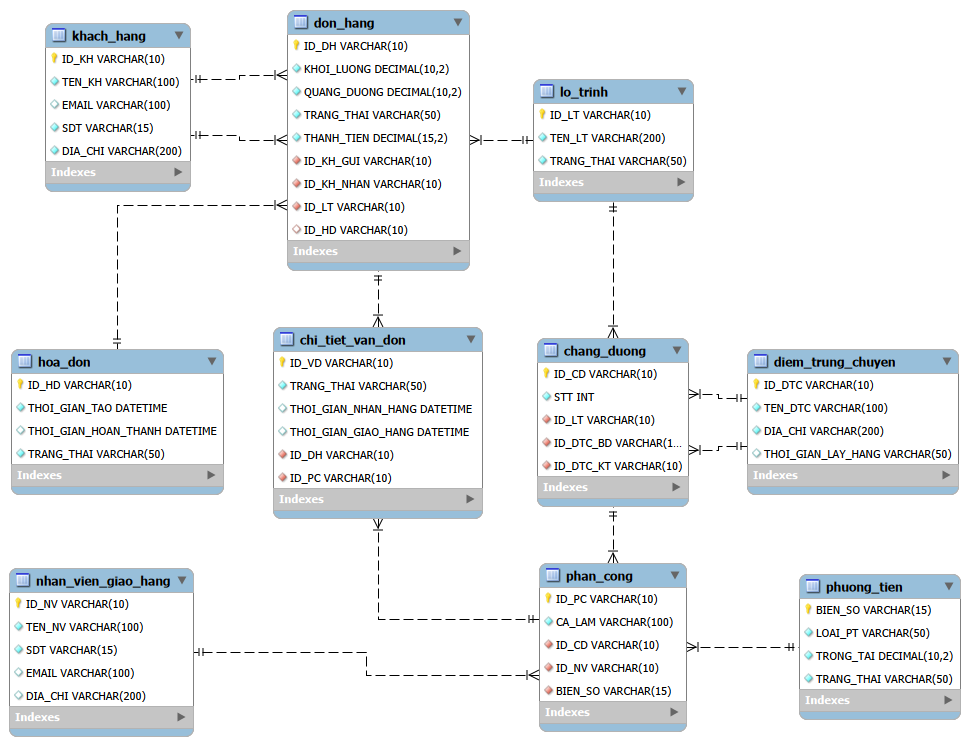
\includegraphics[width=1.0\textwidth]{eerd.png}
    \caption{Sơ đồ thực thể liên kết mở rộng}
    \label{fig:eerd}
\end{figure}

% ========================================================================================================
% CHƯƠNG 5: TRUY VẤN SQL
% ========================================================================================================

\chapter{Truy vấn SQL}
\label{chap:sql}

\section{Các câu truy vấn SQL}
\label{sec:cac_truyvan}

Bảng~\ref{tab:tong_hop_tv} tóm tắt 10 câu truy vấn và kỹ thuật SQL tương ứng.

\begin{table}[H]
    \rowcolors{2}{teal!5}{white}
    \centering
    \renewcommand{\tabularxcolumn}[1]{m{#1}}
    \begin{tabularx}{\textwidth}{|l|X|X|} \hline
        \rowcolor{teal!30}
        \textbf{TT} & \textbf{Mục đích} & \textbf{Kỹ thuật SQL} \\ \hline
        1  & Tra cứu hành trình vận chuyển của đơn hàng   & JOIN 6 bảng, ORDER BY \\ \hline
        2  & Tính phí vận chuyển COD                      & CASE WHEN phân tầng, ROUND \\ \hline
        3  & Thống kê đơn hàng theo trạng thái            & GROUP BY, COUNT, scalar subquery \\ \hline
        4  & Khách hàng và tổng đơn hàng đã gửi           & LEFT JOIN, GROUP BY, COALESCE \\ \hline
        5  & Phương tiện chưa được phân công              & LEFT JOIN, IS NULL (anti-join) \\ \hline
        6  & Số phân công của nhân viên theo lộ trình     & JOIN 4 bảng, GROUP BY, HAVING \\ \hline
        7  & Tổng tiền hóa đơn (COD + giá trị hàng)       & JOIN, SUM + CASE WHEN lồng nhau \\ \hline
        8  & Khách hàng gửi hàng qua lộ trình HN -- ĐN    & EXISTS subquery \\ \hline
        9  & Top 3 lộ trình theo tổng giá trị hàng        & GROUP BY, SUM, AVG, LIMIT \\ \hline
        10 & Hiệu suất giao hàng của từng nhân viên       & CASE WHEN trong COUNT, NULLIF, LEFT JOIN \\ \hline
    \end{tabularx}
    \caption{Tổng hợp 10 câu truy vấn SQL}
    \label{tab:tong_hop_tv}
\end{table}

% --------------------------------------------------------------------------------------------------------

\subsection{Truy vấn 1: Tra cứu hành trình vận chuyển của một đơn hàng}
\label{subsec:tv1}

\textbf{Mục đích:} Hiển thị đầy đủ hành trình thực tế của đơn hàng \texttt{DH004}: từng chặng theo thứ tự, điểm bắt đầu/kết thúc, nhân viên phụ trách, ca làm việc và trạng thái tại từng chặng.

\textbf{Kỹ thuật SQL:} \texttt{INNER JOIN} 6 bảng (\texttt{DON\_HANG}, \texttt{CHI\_TIET\_VAN\_DON}, \texttt{PHAN\_CONG}, \texttt{CHANG\_DUONG}, \texttt{DIEM\_TRUNG\_CHUYEN} $\times 2$, \texttt{NHAN\_VIEN\_GIAO\_HANG}); \texttt{ORDER BY}.

\begin{minted}{sql}
SELECT
    dh.ID_DH,
    cd.STT             AS So_Thu_Tu_Chang,
    dtc_bd.TEN_DTC     AS Diem_Bat_Dau,
    dtc_kt.TEN_DTC     AS Diem_Ket_Thuc,
    nv.TEN_NV          AS Nhan_Vien,
    pc.CA_LAM,
    vd.TRANG_THAI,
    vd.THOI_GIAN_NHAN_HANG,
    vd.THOI_GIAN_GIAO_HANG
FROM DON_HANG dh
    JOIN CHI_TIET_VAN_DON    vd     ON dh.ID_DH    = vd.ID_DH
    JOIN PHAN_CONG           pc     ON vd.ID_PC     = pc.ID_PC
    JOIN CHANG_DUONG         cd     ON pc.ID_CD     = cd.ID_CD
    JOIN DIEM_TRUNG_CHUYEN   dtc_bd ON cd.ID_DTC_BD = dtc_bd.ID_DTC
    JOIN DIEM_TRUNG_CHUYEN   dtc_kt ON cd.ID_DTC_KT = dtc_kt.ID_DTC
    JOIN NHAN_VIEN_GIAO_HANG nv     ON pc.ID_NV     = nv.ID_NV
WHERE dh.ID_DH = 'DH004'
ORDER BY cd.STT;
\end{minted}

Màn hình thực thi của kết quả Truy vấn 1 xem tại Hình~\ref{fig:sql_a1}.

\begin{figure}[H]
    \centering
    \includegraphics[width=1\textwidth]{sql_a1.png}
    \caption{Kết quả Truy vấn 1 --- Hành trình vận chuyển đơn hàng DH004}
    \label{fig:sql_a1}
\end{figure}

% --------------------------------------------------------------------------------------------------------

\subsection{Truy vấn 2: Tính phí vận chuyển (COD) cho tất cả đơn hàng}
\label{subsec:tv2}

\textbf{Mục đích:} Tính phí vận chuyển (thuộc tính dẫn xuất \texttt{COD}, không lưu trong CSDL) cho từng đơn hàng theo công thức phân tầng khoảng cách, tham chiếu bảng cước Viettel Post~\cite{ViettelPostTraCuoc}:

\begin{itemize}
    \item Phí khối lượng: $5.000\ \text{VNĐ/kg}$
    
    \item Phí khoảng cách: $1.000$ VNĐ/km (nếu $\leq 100$ km); $800$ VNĐ/km (101--300 km); $600$ VNĐ/km (trên 300 km)
    
    \item Làm tròn đến nghìn đồng gần nhất.
\end{itemize}

\textbf{Kỹ thuật SQL:} \texttt{CASE WHEN} để phân tầng khoảng cách, hàm \texttt{ROUND()}.

\begin{minted}{sql}
SELECT
    ID_DH,
    KHOI_LUONG,
    QUANG_DUONG,
    ROUND(
        KHOI_LUONG * 5000 +
        CASE
            WHEN QUANG_DUONG <= 100 THEN QUANG_DUONG * 1000
            WHEN QUANG_DUONG <= 300 THEN 100000 + (QUANG_DUONG - 100) * 800
            ELSE                         260000 + (QUANG_DUONG - 300) * 600
        END
    , -3) AS COD_VND
FROM DON_HANG
ORDER BY COD_VND DESC;
\end{minted}

Màn hình thực thi của kết quả Truy vấn 2 xem tại Hình~\ref{fig:sql_a2}.

\begin{figure}[H]
    \centering
    \includegraphics[width=0.5\textwidth]{sql_a2.png}
    \caption{Kết quả Truy vấn 2 --- Phí vận chuyển COD của các đơn hàng}
    \label{fig:sql_a2}
\end{figure}

% --------------------------------------------------------------------------------------------------------

\subsection{Truy vấn 3: Thống kê số lượng đơn hàng theo trạng thái}
\label{subsec:tv3}

\textbf{Mục đích:} Đếm số đơn hàng theo từng trạng thái và tính tỉ lệ phần trăm so với tổng số, giúp quản lý nắm được tổng quan tiến độ xử lý đơn hàng.

\textbf{Kỹ thuật SQL:} \texttt{GROUP BY}, \texttt{COUNT()}, truy vấn con vô hướng (scalar subquery) trong mệnh đề \texttt{SELECT}.

\begin{minted}{sql}
SELECT
    TRANG_THAI,
    COUNT(*)                                           AS So_Don_Hang,
    ROUND(COUNT(*) * 100.0 /
          (SELECT COUNT(*) FROM DON_HANG), 1)         AS Ti_Le_Phan_Tram
FROM DON_HANG
GROUP BY TRANG_THAI
ORDER BY So_Don_Hang DESC;
\end{minted}

Màn hình thực thi của kết quả Truy vấn 3 xem tại Hình~\ref{fig:sql_a3}.

\begin{figure}[H]
    \centering
    \includegraphics[width=0.5\textwidth]{sql_a3.png}
    \caption{Kết quả Truy vấn 3 --- Thống kê đơn hàng theo trạng thái}
    \label{fig:sql_a3}
\end{figure}

% --------------------------------------------------------------------------------------------------------

\subsection{Truy vấn 4: Khách hàng và tổng số đơn hàng đã gửi}
\label{subsec:tv4}

\textbf{Mục đích:} Liệt kê tất cả khách hàng --- kể cả chưa gửi đơn nào --- kèm số đơn hàng đã gửi và tổng giá trị hàng hóa, phục vụ phân tích tệp khách hàng.

\textbf{Kỹ thuật SQL:} \texttt{LEFT JOIN} (giữ lại khách hàng chưa có đơn hàng), \texttt{GROUP BY}, \texttt{COUNT()}, \texttt{SUM()}, \texttt{COALESCE()} xử lý giá trị \texttt{NULL}.

\begin{minted}{sql}
SELECT
    kh.ID_KH,
    kh.TEN_KH,
    kh.SDT,
    COUNT(dh.ID_DH)                    AS So_Don_Da_Gui,
    COALESCE(SUM(dh.THANH_TIEN), 0)    AS Tong_Gia_Tri_Hang_VND
FROM KHACH_HANG kh
    LEFT JOIN DON_HANG dh ON kh.ID_KH = dh.ID_KH_GUI
GROUP BY kh.ID_KH, kh.TEN_KH, kh.SDT
ORDER BY So_Don_Da_Gui DESC, Tong_Gia_Tri_Hang_VND DESC;
\end{minted}

Màn hình thực thi của kết quả Truy vấn 4 xem tại Hình~\ref{fig:sql_a4}.

\begin{figure}[H]
    \centering
    \includegraphics[width=0.75\textwidth]{sql_a4.png}
    \caption{Kết quả Truy vấn 4 --- Khách hàng và tổng đơn hàng đã gửi}
    \label{fig:sql_a4}
\end{figure}

% --------------------------------------------------------------------------------------------------------

\subsection{Truy vấn 5: Phương tiện chưa có phân công trong hệ thống}
\label{subsec:tv5}

\textbf{Mục đích:} Phát hiện phương tiện chưa từng được giao bất kỳ phân công nào --- hỗ trợ quản lý nhận diện phương tiện nhàn rỗi hoặc chưa đưa vào khai thác.

\textbf{Kỹ thuật SQL:} \texttt{LEFT JOIN} kết hợp \texttt{WHERE IS NULL} --- mẫu anti-join phổ biến trong SQL.

\begin{minted}{sql}
SELECT
    pt.BIEN_SO,
    pt.LOAI_PT,
    pt.TRONG_TAI    AS Trong_Tai_Kg,
    pt.TRANG_THAI
FROM PHUONG_TIEN pt
    LEFT JOIN PHAN_CONG pc ON pt.BIEN_SO = pc.BIEN_SO
WHERE pc.ID_PC IS NULL;
\end{minted}

Màn hình thực thi của kết quả Truy vấn 5 xem tại Hình~\ref{fig:sql_a5}.

\begin{figure}[H]
    \centering
    \includegraphics[width=0.5\textwidth]{sql_a5.png}
    \caption{Kết quả Truy vấn 5 --- Phương tiện chưa được phân công}
    \label{fig:sql_a5}
\end{figure}

% --------------------------------------------------------------------------------------------------------

\subsection{Truy vấn 6: Số phân công của từng nhân viên theo lộ trình}
\label{subsec:tv6}

\textbf{Mục đích:} Thống kê số lần mỗi nhân viên được phân công, phân nhóm theo lộ trình, chỉ lấy các nhóm có ít nhất 2 phân công --- đánh giá mức độ tham gia thực tế của nhân sự.

\textbf{Kỹ thuật SQL:} \texttt{JOIN} 4 bảng, \texttt{GROUP BY} nhiều cột, \texttt{HAVING} lọc nhóm, \texttt{ORDER BY} đa tiêu chí.

\begin{minted}{sql}
SELECT
    nv.ID_NV,
    nv.TEN_NV,
    lt.TEN_LT               AS Lo_Trinh,
    COUNT(pc.ID_PC)         AS So_Phan_Cong
FROM NHAN_VIEN_GIAO_HANG nv
    JOIN PHAN_CONG   pc ON nv.ID_NV = pc.ID_NV
    JOIN CHANG_DUONG cd ON pc.ID_CD = cd.ID_CD
    JOIN LO_TRINH    lt ON cd.ID_LT = lt.ID_LT
GROUP BY nv.ID_NV, nv.TEN_NV, lt.ID_LT, lt.TEN_LT
HAVING COUNT(pc.ID_PC) >= 2
ORDER BY So_Phan_Cong DESC, nv.ID_NV;
\end{minted}

Màn hình thực thi của kết quả Truy vấn 6 xem tại Hình~\ref{fig:sql_a6}.

\begin{figure}[H]
    \centering
    \includegraphics[width=0.5\textwidth]{sql_a6.png}
    \caption{Kết quả Truy vấn 6 --- Số phân công của nhân viên theo lộ trình}
    \label{fig:sql_a6}
\end{figure}

% --------------------------------------------------------------------------------------------------------

\subsection{Truy vấn 7: Tổng tiền từng hóa đơn (COD + giá trị hàng)}
\label{subsec:tv7}

\textbf{Mục đích:} Tính tổng tiền phải thanh toán của từng hóa đơn theo công thức $\texttt{TONG\_TIEN} = \sum(\texttt{COD} + \texttt{THANH\_TIEN})$ trên toàn bộ đơn hàng thuộc hóa đơn đó.

\textbf{Kỹ thuật SQL:} \texttt{JOIN}, \texttt{GROUP BY}, \texttt{SUM()} kết hợp biểu thức \texttt{CASE WHEN} lồng nhau để tính COD, \texttt{ROUND()}.

\begin{minted}{sql}
SELECT
    hd.ID_HD,
    hd.TRANG_THAI             AS Trang_Thai_Hoa_Don,
    COUNT(dh.ID_DH)           AS So_Don_Hang,
    ROUND(SUM(
        dh.KHOI_LUONG * 5000 +
        CASE
            WHEN dh.QUANG_DUONG <= 100
                THEN dh.QUANG_DUONG * 1000
            WHEN dh.QUANG_DUONG <= 300
                THEN 100000 + (dh.QUANG_DUONG - 100) * 800
            ELSE     260000 + (dh.QUANG_DUONG - 300) * 600
        END
    ), -3)                    AS Tong_COD_VND,
    SUM(dh.THANH_TIEN)        AS Tong_Gia_Tri_Hang_VND,
    ROUND(SUM(
        dh.KHOI_LUONG * 5000 +
        CASE
            WHEN dh.QUANG_DUONG <= 100
                THEN dh.QUANG_DUONG * 1000
            WHEN dh.QUANG_DUONG <= 300
                THEN 100000 + (dh.QUANG_DUONG - 100) * 800
            ELSE     260000 + (dh.QUANG_DUONG - 300) * 600
        END
    ) + SUM(dh.THANH_TIEN), -3) AS TONG_TIEN_VND
FROM HOA_DON hd
    JOIN DON_HANG dh ON hd.ID_HD = dh.ID_HD
GROUP BY hd.ID_HD, hd.TRANG_THAI
ORDER BY TONG_TIEN_VND DESC;
\end{minted}

Màn hình thực thi của kết quả Truy vấn 7 xem tại Hình~\ref{fig:sql_a7}.

\begin{figure}[H]
    \centering
    \includegraphics[width=\textwidth]{sql_a7.png}
    \caption{Kết quả Truy vấn 7 --- Tổng tiền từng hóa đơn}
    \label{fig:sql_a7}
\end{figure}

% --------------------------------------------------------------------------------------------------------

\subsection{Truy vấn 8: Khách hàng đã gửi hàng qua lộ trình Hà Nội -- Đà Nẵng}
\label{subsec:tv8}

\textbf{Mục đích:} Tìm danh sách khách hàng đã từng gửi ít nhất một đơn hàng đi theo lộ trình có tuyến Hà Nội -- Đà Nẵng (bao gồm cả \texttt{LT001} và \texttt{LT004}), phục vụ chăm sóc khách hàng định tuyến.

\textbf{Kỹ thuật SQL:} Subquery với \texttt{EXISTS} --- kiểm tra sự tồn tại của bản ghi thỏa điều kiện mà không cần \texttt{JOIN} bảng ngoài, thường hiệu quả hơn \texttt{IN} với tập kết quả lớn.

\begin{minted}{sql}
SELECT
    kh.ID_KH,
    kh.TEN_KH,
    kh.SDT,
    kh.DIA_CHI
FROM KHACH_HANG kh
WHERE EXISTS (
    SELECT 1
    FROM DON_HANG dh
        JOIN LO_TRINH lt ON dh.ID_LT = lt.ID_LT
    WHERE dh.ID_KH_GUI = kh.ID_KH
      AND lt.TEN_LT LIKE '%Ha Noi - Da Nang%'
)
ORDER BY kh.ID_KH;
\end{minted}

Màn hình thực thi của kết quả Truy vấn 8 xem tại Hình~\ref{fig:sql_a8}.

\begin{figure}[H]
    \centering
    \includegraphics[width=0.75\textwidth]{sql_a8.png}
    \caption{Kết quả Truy vấn 8 --- Khách hàng gửi hàng qua lộ trình HN -- ĐN}
    \label{fig:sql_a8}
\end{figure}

% --------------------------------------------------------------------------------------------------------

\subsection{Truy vấn 9: Top 3 lộ trình có tổng giá trị hàng hóa cao nhất}
\label{subsec:tv9}

\textbf{Mục đích:} Xếp hạng 3 lộ trình có tổng giá trị hàng vận chuyển lớn nhất, kèm số đơn hàng và khối lượng trung bình --- hỗ trợ lãnh đạo ưu tiên đầu tư phương tiện và nhân lực cho các tuyến trọng điểm.

\textbf{Kỹ thuật SQL:} \texttt{JOIN}, \texttt{GROUP BY}, \texttt{SUM()}, \texttt{AVG()}, \texttt{COUNT()}, \texttt{ORDER BY} kết hợp \texttt{LIMIT}.

\begin{minted}{sql}
SELECT
    lt.ID_LT,
    lt.TEN_LT,
    COUNT(dh.ID_DH)               AS So_Don_Hang,
    ROUND(AVG(dh.KHOI_LUONG), 2)  AS KL_Trung_Binh_Kg,
    SUM(dh.THANH_TIEN)            AS Tong_Gia_Tri_Hang_VND
FROM LO_TRINH lt
    JOIN DON_HANG dh ON lt.ID_LT = dh.ID_LT
GROUP BY lt.ID_LT, lt.TEN_LT
ORDER BY Tong_Gia_Tri_Hang_VND DESC
LIMIT 3;
\end{minted}

Màn hình thực thi của kết quả Truy vấn 9 xem tại Hình~\ref{fig:sql_a9}.

\begin{figure}[H]
    \centering
    \includegraphics[width=\textwidth]{sql_a9.png}
    \caption{Kết quả Truy vấn 9 --- Top 3 lộ trình theo tổng giá trị hàng}
    \label{fig:sql_a9}
\end{figure}

% --------------------------------------------------------------------------------------------------------

\subsection{Truy vấn 10: Báo cáo hiệu suất giao hàng của từng nhân viên}
\label{subsec:tv10}

\textbf{Mục đích:} Tổng hợp KPI vận hành: số lượt giao hàng, phân loại theo kết quả (\texttt{Da giao} / \texttt{Dang van chuyen} / \texttt{Hoan tra}) và tỉ lệ thành công của từng nhân viên, bao gồm cả nhân viên chưa có lượt giao nào.

\textbf{Kỹ thuật SQL:} \texttt{LEFT JOIN} nhiều bảng; \texttt{CASE WHEN} lồng trong \texttt{COUNT(DISTINCT ...)} để đếm có điều kiện; \texttt{NULLIF()} tránh lỗi chia cho 0; \texttt{GROUP BY}; \texttt{ORDER BY} đa tiêu chí.

\begin{minted}{sql}
SELECT
    nv.ID_NV,
    nv.TEN_NV,
    COUNT(DISTINCT vd.ID_VD)                        AS Tong_Luot_Giao,
    COUNT(DISTINCT CASE
        WHEN vd.TRANG_THAI = 'Da giao'
        THEN vd.ID_VD END)                          AS So_Da_Giao,
    COUNT(DISTINCT CASE
        WHEN vd.TRANG_THAI = 'Dang van chuyen'
        THEN vd.ID_VD END)                          AS So_Dang_Van_Chuyen,
    COUNT(DISTINCT CASE
        WHEN vd.TRANG_THAI = 'Hoan tra'
        THEN vd.ID_VD END)                          AS So_Hoan_Tra,
    ROUND(
        COUNT(DISTINCT CASE
            WHEN vd.TRANG_THAI = 'Da giao'
            THEN vd.ID_VD END) * 100.0 /
        NULLIF(COUNT(DISTINCT vd.ID_VD), 0)
    , 1)                                            AS Ti_Le_Thanh_Cong
FROM NHAN_VIEN_GIAO_HANG nv
    LEFT JOIN PHAN_CONG        pc ON nv.ID_NV = pc.ID_NV
    LEFT JOIN CHI_TIET_VAN_DON vd ON pc.ID_PC = vd.ID_PC
GROUP BY nv.ID_NV, nv.TEN_NV
ORDER BY Ti_Le_Thanh_Cong DESC, Tong_Luot_Giao DESC;
\end{minted}

Màn hình thực thi của kết quả Truy vấn 10 xem tại Hình~\ref{fig:sql_a10}.

\begin{figure}[H]
    \centering
    \includegraphics[width=\textwidth]{sql_a10.png}
    \caption{Kết quả Truy vấn 10 --- Hiệu suất giao hàng của từng nhân viên}
    \label{fig:sql_a10}
\end{figure}

% ========================================================================================================
% CHƯƠNG 6: LẬP TRÌNH SQL NÂNG CAO VÀ BẢO MẬT TRONG MYSQL
% ========================================================================================================

\chapter{Lập trình SQL nâng cao và Bảo mật trong MySQL}
\label{chap:tsql}

Chương này trình bày hai nội dung tự nghiên cứu: 
\begin{enumerate}
    \item Lập trình SQL thủ tục theo chuẩn T-SQL và cách MySQL hiện thực hóa các khái niệm tương đương;
    \item Các cơ chế bảo mật cơ sở dữ liệu. 
\end{enumerate}
Minh họa bằng ví dụ cụ thể trên CSDL \texttt{cargo\_db} đã xây dựng tại Chương~\ref{chap:sql}.

% ============================================================
\section{T-SQL và lập trình thủ tục trong cơ sở dữ liệu}
\label{sec:tsql}

\subsection{Tổng quan về T-SQL}
\label{subsec:tsql_tq}

\textbf{T-SQL} (Transact-SQL) là ngôn ngữ lập trình thủ tục do Microsoft phát triển, mở rộng SQL chuẩn (SQL-92/SQL:1999) cho hệ quản trị cơ sở dữ liệu SQL Server~\cite{mssql_tsql}. T-SQL bổ sung các tính năng không có trong SQL chuẩn: biến cục bộ, cấu trúc điều khiển (IF/WHILE), xử lý ngoại lệ (TRY...CATCH), con trỏ (cursor), thủ tục lưu trữ, hàm do người dùng định nghĩa và trigger.

MySQL --- hệ quản trị đang sử dụng trong báo cáo này --- cũng cung cấp đầy đủ hệ thống lập trình thủ tục tương đương, gọi là \textbf{MySQL Procedural Language}~\cite{mysql80_sproc}. Hai ngôn ngữ có cùng triết lý thiết kế nhưng khác nhau về cú pháp. Bảng~\ref{tab:tsql_vs_mysql} so sánh các cấu trúc cốt lõi.

\begin{table}[H]
    \rowcolors{2}{teal!5}{white}
    \centering
    \renewcommand{\tabularxcolumn}[1]{m{#1}}
    \begin{tabularx}{\textwidth}{|l|>{\raggedright\arraybackslash}X|>{\raggedright\arraybackslash}X|} \hline
        \rowcolor{teal!30}
        \textbf{Cấu trúc} & \textbf{T-SQL (SQL Server)} & \textbf{MySQL} \\ \hline
        Khai báo biến     & \texttt{DECLARE @v INT}                             & \texttt{DECLARE v INT}              \\ \hline
        Gán giá trị       & \texttt{SET @v = 1}                                 & \texttt{SET v = 1}                  \\ \hline
        Rẽ nhánh          & \texttt{IF ... BEGIN ... END}                       & \texttt{IF ... THEN ... END IF}     \\ \hline
        Vòng lặp          & \texttt{WHILE ... BEGIN ... END}                    & \texttt{WHILE ... DO ... END WHILE} \\ \hline
        Xử lý lỗi         & \texttt{TRY ... CATCH}                              & \texttt{DECLARE ... HANDLER FOR}    \\ \hline
        Báo lỗi tùy chỉnh & \texttt{RAISERROR(...)}                             & \texttt{SIGNAL SQLSTATE '45000'}    \\ \hline
        Procedure         & \texttt{CREATE PROCEDURE p AS BEGIN...END}          & \texttt{CREATE PROCEDURE p() BEGIN...END} \\ \hline
        Function          & \texttt{CREATE FUNCTION f() RETURNS INT AS...}      & \texttt{CREATE FUNCTION f() RETURNS INT DETERMINISTIC...} \\ \hline
        Trigger           & \texttt{CREATE TRIGGER t ON tbl AFTER INSERT AS...} & \texttt{CREATE TRIGGER t AFTER INSERT ON tbl FOR EACH ROW...} \\ \hline
        Phân cách lệnh    & Không cần \texttt{DELIMITER}                        & Cần \texttt{DELIMITER \$\$}         \\ \hline
        In kết quả        & \texttt{PRINT 'msg'}                                & \texttt{SELECT 'msg'}               \\ \hline
    \end{tabularx}
    \caption{So sánh cú pháp T-SQL (SQL Server) và MySQL Procedural Language}
    \label{tab:tsql_vs_mysql}
\end{table}

\subsection{Các cấu trúc lập trình cơ bản trong MySQL}
\label{subsec:cautruc_cb}

Trước khi đi vào ví dụ, đây là bộ cú pháp cốt lõi của MySQL Procedural Language minh họa biến, điều kiện, vòng lặp và xử lý lỗi --- tương đương với các khái niệm cùng tên trong T-SQL:

\begin{minted}{sql}
-- Cu phap T-SQL (SQL Server)
DECLARE @tong_don INT = 0;          -- khai bao + khoi tao
SET     @tong_don = @tong_don + 1;  -- gan gia tri

IF @tong_don > 10
BEGIN
    PRINT N'Co nhieu hon 10 don hang';
END
ELSE
BEGIN
    PRINT N'It hon hoac bang 10 don hang';
END;

WHILE @tong_don < 20
BEGIN
    SET @tong_don = @tong_don + 1;
END;
\end{minted}

Cú pháp tương đương trong MySQL:

\begin{minted}{sql}
-- Cu phap tuong duong trong MySQL
DECLARE v_tong_don INT DEFAULT 0;         -- khai bao + khoi tao
SET     v_tong_don = v_tong_don + 1;      -- gan gia tri

IF v_tong_don > 10 THEN
    SELECT 'Co nhieu hon 10 don hang' AS Thong_Bao;
ELSE
    SELECT 'It hon hoac bang 10 don hang' AS Thong_Bao;
END IF;

WHILE v_tong_don < 20 DO
    SET v_tong_don = v_tong_don + 1;
END WHILE;

-- Bao loi tuy chinh (tuong duong RAISERROR trong T-SQL)
SIGNAL SQLSTATE '45000'
    SET MESSAGE_TEXT = 'Loi nghiep vu: du lieu khong hop le!';
\end{minted}

Để minh họa T-SQL đúng nghĩa, phần này viết lại hai ví dụ xuyên suốt chương theo đúng cú pháp SQL Server trước khi trình bày phiên bản MySQL tương đương tại các Mục~\ref{subsec:ex_function} và~\ref{subsec:ex_sproc}.

\subsection{Ví dụ 1 --- Hàm tính phí vận chuyển \texttt{fn\_TinhCOD()}}
\label{subsec:ex_function}

\textbf{Đặt vấn đề:} \texttt{COD} là thuộc tính dẫn xuất --- không lưu trong CSDL mà tính khi cần. Mỗi lần tính phải lặp lại biểu thức \texttt{CASE WHEN} phức tạp trong mọi câu truy vấn (đã thấy ở Truy vấn 2 và 7, Chương~\ref{chap:sql}). Giải pháp: đóng gói công thức thành một \textbf{hàm do người dùng định nghĩa (UDF)} để tái sử dụng.

\textbf{Công thức COD} tham chiếu bảng cước Viettel Post~\cite{ViettelPostTraCuoc}: phí khối lượng $5.000\ \text{VNĐ/kg}$, cộng phí khoảng cách phân tầng ($1.000$/$800$/$600$ VNĐ/km), làm tròn đến nghìn đồng.

Trong T-SQL, hàm do người dùng định nghĩa (UDF) không cần \texttt{DELIMITER}, dùng tiền tố \texttt{@} cho biến và gọi qua tiền tố schema \texttt{dbo.}~\cite{mssql_tsql}.

\begin{minted}{sql}
CREATE FUNCTION dbo.fn_TinhCOD_TSQL(
    @p_khoi_luong   DECIMAL(10,2),
    @p_quang_duong  DECIMAL(10,2)
)
RETURNS DECIMAL(15,2)
WITH SCHEMABINDING          -- rang buoc schema, ho tro toi uu hoa
AS
BEGIN
    DECLARE @v_phi_kl   DECIMAL(15,2);  -- phi khoi luong
    DECLARE @v_phi_qd   DECIMAL(15,2);  -- phi khoang cach
    DECLARE @v_cod      DECIMAL(15,2);  -- ket qua cuoi

    -- Phi theo khoi luong: 5.000 VND/kg
    SET @v_phi_kl = @p_khoi_luong * 5000;

    -- Phi theo khoang cach (phan tang, theo bang cuoc Viettel Post)
    SET @v_phi_qd =
        CASE
            WHEN @p_quang_duong <= 100
                 THEN @p_quang_duong * 1000
            WHEN @p_quang_duong <= 300
                 THEN 100000 + (@p_quang_duong - 100) * 800
            ELSE
                 260000 + (@p_quang_duong - 300) * 600
        END;

    -- Lam tron den nghin dong gan nhat (ROUND voi do chinh xac -3)
    SET @v_cod = ROUND(@v_phi_kl + @v_phi_qd, -3);
    RETURN @v_cod;
END;
GO

-- Goi ham trong T-SQL (phai co tien to schema dbo.):
SELECT
    ID_DH,
    KHOI_LUONG,
    QUANG_DUONG,
    dbo.fn_TinhCOD_TSQL(KHOI_LUONG, QUANG_DUONG)   AS COD_VND,
    THANH_TIEN,
    dbo.fn_TinhCOD_TSQL(KHOI_LUONG, QUANG_DUONG)
        + THANH_TIEN                                AS Tong_Thu_Tu_KH
FROM DON_HANG
ORDER BY COD_VND DESC;
\end{minted}

Cú pháp tương đương trong MySQL:

\begin{minted}{sql}
-- Doi delimiter de MySQL khong nham ';' ben trong la ket thuc lenh
DELIMITER //

CREATE FUNCTION fn_TinhCOD(
    p_khoi_luong   DECIMAL(10,2),
    p_quang_duong  DECIMAL(10,2)
)
RETURNS DECIMAL(15,2)
DETERMINISTIC       -- cung input -> cung output, khong phu thuoc trang thai DB
COMMENT 'Tinh phi van chuyen (COD) theo cong thuc phan tang khoang cach Viettel Post'
BEGIN
    DECLARE v_phi_kl    DECIMAL(15,2);  -- phi khoi luong
    DECLARE v_phi_qd    DECIMAL(15,2);  -- phi khoang cach
    DECLARE v_cod       DECIMAL(15,2);  -- ket qua cuoi

    -- Phi theo khoi luong: 5.000 VND/kg
    SET v_phi_kl = p_khoi_luong * 5000;

    -- Phi theo khoang cach (phan tang)
    SET v_phi_qd =
        CASE
            WHEN p_quang_duong <= 100
                THEN p_quang_duong * 1000
            WHEN p_quang_duong <= 300
                THEN 100000 + (p_quang_duong - 100) * 800
            ELSE
                260000 + (p_quang_duong - 300) * 600
        END;

    -- Tong phi, lam tron den nghin dong gan nhat
    SET v_cod = ROUND(v_phi_kl + v_phi_qd, -3);
    RETURN v_cod;
END//

DELIMITER ;
\end{minted}

Sau khi tạo hàm, các câu truy vấn trở nên ngắn gọn hơn đáng kể:

\begin{minted}{sql}
-- Su dung ham fn_TinhCOD trong truy van (thay cho bieu thuc CASE WHEN dai)
SELECT
    ID_DH,
    KHOI_LUONG,
    QUANG_DUONG,
    fn_TinhCOD(KHOI_LUONG, QUANG_DUONG)   AS COD_VND,
    THANH_TIEN,
    fn_TinhCOD(KHOI_LUONG, QUANG_DUONG)
        + THANH_TIEN                       AS Tong_Thu_Tu_KH
FROM DON_HANG
ORDER BY COD_VND DESC;
\end{minted}

\begin{figure}[H]
    \centering
    \includegraphics[width=0.75\textwidth]{vd1.png}
    \caption{Sử dụng hàm fn\_TinhCOD trong truy vấn}
\end{figure}

\subsection{Ví dụ 2 --- Thủ tục lưu trữ tra cứu đơn hàng \texttt{sp\_ThongKeDonHang()}}
\label{subsec:ex_sproc}

\textbf{Đặt vấn đề:} Quản lý thường xuyên cần tra cứu danh sách đơn hàng theo trạng thái và biết tổng số đơn hàng tương ứng. Thay vì viết nhiều câu truy vấn rời rạc, đóng gói thành \textbf{Stored Procedure} với tham số đầu vào linh hoạt và trả về kết quả qua tham số đầu ra \texttt{OUT}~\cite{mysql80_sproc}.

Thủ tục lưu trữ trong T-SQL dùng từ khóa \texttt{OUTPUT} thay vì \texttt{OUT}, và \texttt{SET NOCOUNT ON} để tắt thông báo số dòng bị ảnh hưởng~\cite{mssql_tsql}.

\begin{minted}{sql}
CREATE PROCEDURE dbo.sp_ThongKeDonHang_TSQL
    @p_trang_thai NVARCHAR(50) = NULL,  -- NULL = lay tat ca trang thai
    @p_so_luong   INT          OUTPUT   -- tham so dau ra (T-SQL dung OUTPUT)
AS
BEGIN
    SET NOCOUNT ON;  -- tat thong bao so dong bi anh huong (khac MySQL)

    -- Phan 1: Hien thi danh sach chi tiet
    SELECT
        dh.ID_DH,
        kh_gui.TEN_KH                                        AS Nguoi_Gui,
        kh_nhan.TEN_KH                                       AS Nguoi_Nhan,
        lt.TEN_LT                                            AS Lo_Trinh,
        dh.KHOI_LUONG,
        dbo.fn_TinhCOD_TSQL(dh.KHOI_LUONG, dh.QUANG_DUONG)  AS COD_VND,
        dh.TRANG_THAI
    FROM DON_HANG dh
        JOIN KHACH_HANG kh_gui  ON dh.ID_KH_GUI  = kh_gui.ID_KH
        JOIN KHACH_HANG kh_nhan ON dh.ID_KH_NHAN = kh_nhan.ID_KH
        JOIN LO_TRINH   lt      ON dh.ID_LT       = lt.ID_LT
    WHERE @p_trang_thai IS NULL
       OR dh.TRANG_THAI = @p_trang_thai
    ORDER BY dh.ID_DH;

    -- Phan 2: Dem tong so luong, tra ve qua tham so OUTPUT
    SELECT @p_so_luong = COUNT(*)
    FROM DON_HANG
    WHERE @p_trang_thai IS NULL
       OR TRANG_THAI = @p_trang_thai;
END;
GO

-- Goi thu tuc trong T-SQL (dung EXEC va OUTPUT):
DECLARE @tong INT;
EXEC dbo.sp_ThongKeDonHang_TSQL
    @p_trang_thai = N'Da giao',
    @p_so_luong   = @tong OUTPUT;

-- In ket qua (T-SQL dung PRINT + CAST thay vi SELECT):
PRINT N'Tong don hang Da giao: ' + CAST(@tong AS NVARCHAR(10));
\end{minted}

Cú pháp tương đương trong MySQL:

\begin{minted}{sql}
DELIMITER //

CREATE PROCEDURE sp_ThongKeDonHang(
    IN  p_trang_thai  VARCHAR(50),  -- NULL = lay tat ca trang thai
    OUT p_so_luong    INT           -- Tra ve tong so don hang tim duoc
)
COMMENT 'Tra cuu don hang theo trang thai, tra ve danh sach va tong so luong'
BEGIN
    -- Hien thi danh sach chi tiet
    SELECT
        dh.ID_DH,
        kh_gui.TEN_KH                               AS Nguoi_Gui,
        kh_nhan.TEN_KH                              AS Nguoi_Nhan,
        lt.TEN_LT                                   AS Lo_Trinh,
        dh.KHOI_LUONG,
        fn_TinhCOD(dh.KHOI_LUONG, dh.QUANG_DUONG)  AS COD_VND,
        dh.TRANG_THAI
    FROM DON_HANG dh
        JOIN KHACH_HANG kh_gui  ON dh.ID_KH_GUI  = kh_gui.ID_KH
        JOIN KHACH_HANG kh_nhan ON dh.ID_KH_NHAN = kh_nhan.ID_KH
        JOIN LO_TRINH   lt      ON dh.ID_LT       = lt.ID_LT
    WHERE p_trang_thai IS NULL
       OR dh.TRANG_THAI = p_trang_thai
    ORDER BY dh.ID_DH;

    -- Phan 2: Dem tong so luong va gan vao bien OUT
    SELECT COUNT(*) INTO p_so_luong
    FROM DON_HANG
    WHERE p_trang_thai IS NULL
       OR TRANG_THAI = p_trang_thai;
END//

DELIMITER ;

-- Cach goi thu tuc:

-- 1. Lay tat ca don hang 'Da giao' va biet tong so luong
CALL sp_ThongKeDonHang('Da giao', @tong);
SELECT @tong AS Tong_Don_Da_Giao;

-- 2. Lay tat ca don hang khong loc trang thai (truyen NULL)
CALL sp_ThongKeDonHang(NULL, @tong);
SELECT @tong AS Tong_Toan_Bo_Don_Hang;
\end{minted}

\begin{figure}[H]
    \centering
    \includegraphics[width=\textwidth]{vd2-1.png}
    \caption{Lấy tất cả đơn hàng \texttt{'Da giao'}}
\end{figure}

\begin{figure}[H]
    \centering
    \includegraphics[width=0.25\textwidth]{vd2-2.png}
    \caption{Số lượng tất cả đơn hàng \texttt{'Da giao'}}
\end{figure}

\textbf{Tổng hợp điểm khác biệt chính giữa T-SQL và MySQL} rút ra từ hai ví dụ trên:
\begin{itemize}
    \item \textbf{Tiền tố biến:} T-SQL dùng \texttt{@} (ví dụ \texttt{@v\_cod}); MySQL dùng tên thuần (\texttt{v\_cod}).
    \item \textbf{Kết thúc block:} T-SQL dùng \texttt{AS BEGIN \ldots{} END} + \texttt{GO}; MySQL cần \texttt{DELIMITER \$\$} và \texttt{BEGIN \ldots{} END\$\$}.
    \item \textbf{Tham số đầu ra:} T-SQL dùng từ khóa \texttt{OUTPUT}; MySQL dùng \texttt{OUT}.
    \item \textbf{Gọi hàm:} T-SQL yêu cầu tiền tố schema \texttt{dbo.fn\_TinhCOD\_TSQL(...)}; MySQL gọi trần tên hàm.
    \item \textbf{In thông báo:} T-SQL dùng \texttt{PRINT}; MySQL dùng \texttt{SELECT \ldots{} AS}.
    \item \textbf{Ràng buộc schema:} T-SQL hỗ trợ \texttt{WITH SCHEMABINDING} tối ưu hóa hàm; MySQL không có tương đương trực tiếp (dùng \texttt{DETERMINISTIC}).
\end{itemize}

\subsection{Trigger --- Kiểm soát ràng buộc nghiệp vụ tự động}
\label{subsec:trigger}

\textbf{Trigger} là đối tượng CSDL tự động kích hoạt khi có sự kiện \texttt{INSERT}/\texttt{UPDATE}/\texttt{DELETE} xảy ra trên một bảng~\cite{elmasri2015fundamentals}. Ưu điểm so với kiểm tra ở tầng ứng dụng: ràng buộc được đảm bảo ngay tại tầng CSDL, không phụ thuộc vào ngôn ngữ lập trình phía trên.

Hai ràng buộc nghiệp vụ tại Mục~\ref{subsubsec:check_constraints} không thể biểu diễn bằng \texttt{CHECK} thông thường (vì liên quan nhiều bảng) --- đây là lúc Trigger phát huy tác dụng:

\begin{minted}{sql}
-- Trigger 1: Kiem tra phuong tien phai o trang thai 'Hoat dong'
--            truoc khi tao PHAN_CONG moi
DELIMITER //

CREATE TRIGGER trg_KiemTraPhuongTien
BEFORE INSERT ON PHAN_CONG
FOR EACH ROW
BEGIN
    DECLARE v_trang_thai VARCHAR(50);

    SELECT TRANG_THAI INTO v_trang_thai
    FROM   PHUONG_TIEN
    WHERE  BIEN_SO = NEW.BIEN_SO;

    IF v_trang_thai <> 'Hoat dong' THEN
        SIGNAL SQLSTATE '45000'
        SET MESSAGE_TEXT =
            'Phuong tien khong o trang thai Hoat dong, khong the phan cong!';
    END IF;
END//

DELIMITER ;
\end{minted}

\begin{figure}[H]
    \centering
    \includegraphics[width=0.75\textwidth]{trigger1-2.png}
    \caption{Kết quả hiển thị INSERT thất bại khi phương tiện không ở trạng thái \texttt{'Hoat dong'}}
\end{figure}

\begin{minted}{sql}
-- Trigger 2: Kiem tra chang duong cua phan cong phai thuoc
--            lo trinh ma don hang dang di theo
--            (bao toan tinh nhat quan cua chu trinh trong ERD)
DELIMITER //

CREATE TRIGGER trg_KiemTraHanhTrinh
BEFORE INSERT ON CHI_TIET_VAN_DON
FOR EACH ROW
BEGIN
    DECLARE v_lt_don_hang   VARCHAR(10);
    DECLARE v_lt_phan_cong  VARCHAR(10);

    -- Lo trinh cua don hang
    SELECT ID_LT INTO v_lt_don_hang
    FROM   DON_HANG
    WHERE  ID_DH = NEW.ID_DH;

    -- Lo trinh cua chang duong trong phan cong
    SELECT cd.ID_LT INTO v_lt_phan_cong
    FROM   PHAN_CONG pc
        JOIN CHANG_DUONG cd ON pc.ID_CD = cd.ID_CD
    WHERE  pc.ID_PC = NEW.ID_PC;

    IF v_lt_don_hang <> v_lt_phan_cong THEN
        SIGNAL SQLSTATE '45000'
        SET MESSAGE_TEXT =
            'Chang duong cua phan cong khong thuoc lo trinh cua don hang!';
    END IF;
END//

DELIMITER ;
\end{minted}

\begin{figure}[H]
    \centering
    \includegraphics[width=0.75\textwidth]{trigger2-2.png}
    \caption{Kết quả hiển thị INSERT thất bại khi chặng đường của phân công không thuộc lộ trình của đơn hàng}
\end{figure}

% ============================================================
\section{Bảo mật trong hệ quản trị cơ sở dữ liệu}
\label{sec:baomat}

\subsection{Tổng quan về bảo mật cơ sở dữ liệu}
\label{subsec:baomat_tq}

Bảo mật cơ sở dữ liệu là tập hợp các chính sách, cơ chế và công cụ nhằm đảm bảo ba thuộc tính cốt lõi --- mô hình \textbf{CIA}~\cite{elmasri2015fundamentals}:

\begin{itemize}
    \item \textbf{Confidentiality (Bí mật):} Chỉ người dùng được ủy quyền mới truy cập được dữ liệu. Ví dụ: nhân viên giao hàng không được xem thông tin thanh toán của khách hàng.
    \item \textbf{Integrity (Toàn vẹn):} Dữ liệu chỉ được sửa đổi bởi người có quyền và theo đúng quy trình. Ví dụ: chỉ kế toán mới được cập nhật trạng thái hóa đơn.
    \item \textbf{Availability (Sẵn sàng):} Hệ thống và dữ liệu luôn sẵn sàng phục vụ khi cần. Ví dụ: backup định kỳ để phục hồi khi có sự cố.
\end{itemize}

Các mối đe dọa phổ biến với CSDL bao gồm: \textit{SQL Injection} (chèn câu lệnh SQL độc hại), leo thang đặc quyền, rò rỉ dữ liệu qua tài khoản không an toàn, và mất mát dữ liệu do lỗi phần cứng hoặc tấn công ransomware~\cite{mysql80_security}.

\subsection{Các cơ chế bảo mật trong MySQL}
\label{subsec:baomat_coche}

\begin{table}[H]
    \rowcolors{2}{teal!5}{white}
    \centering
    \renewcommand{\tabularxcolumn}[1]{m{#1}}
    \begin{tabularx}{\textwidth}{|l|>{\raggedright\arraybackslash}X|>{\raggedright\arraybackslash}X|} \hline
        \rowcolor{teal!30}
        \textbf{Cơ chế} & \textbf{Mô tả} & \textbf{Câu lệnh MySQL} \\ \hline
        Xác thực (Authentication)  & Quản lý danh tính người dùng & \texttt{CREATE USER}, \texttt{ALTER USER} \\ \hline
        Phân quyền (Authorization) & Cấp/thu hồi quyền thao tác   & \texttt{GRANT}, \texttt{REVOKE} \\ \hline
        Vai trò (Role)             & Gom nhóm quyền hạn           & \texttt{CREATE ROLE}, \texttt{GRANT role TO user} \\ \hline
        View bảo mật               & Ẩn dữ liệu nhạy cảm qua view & \texttt{CREATE VIEW}, kết hợp với \texttt{GRANT} \\ \hline
        Mã hóa dữ liệu             & Mã hóa cột/bảng              & \texttt{AES\_ENCRYPT()}, \texttt{AES\_DECRYPT()} \\ \hline
        Phòng chống SQL Injection  & Tham số hóa câu truy vấn     & Prepared Statements (\texttt{PREPARE}, \texttt{EXECUTE}) \\ \hline
        Backup \& Phục hồi         & Sao lưu và khôi phục dữ liệu & \texttt{mysqldump}, MySQL Enterprise Backup \\ \hline
        Audit Log                  & Ghi lại các thao tác         & MySQL Enterprise Audit / General Query Log \\ \hline
    \end{tabularx}
    \caption{Tổng hợp các cơ chế bảo mật trong MySQL 8.0}
    \label{tab:baomat_coche}
\end{table}

\subsection{Ví dụ 1 --- Phân quyền người dùng theo vai trò}
\label{subsec:ex_grant}

\textbf{Đặt vấn đề:} Hệ thống \texttt{cargo\_db} có nhiều loại người dùng với nhu cầu truy cập khác nhau. Áp dụng \textbf{nguyên tắc đặc quyền tối thiểu} (Principle of Least Privilege): mỗi tài khoản chỉ được cấp đúng quyền cần thiết cho công việc của mình~\cite{mysql80_security}.

\begin{minted}{sql}
-- Buoc 1: Tao cac vai tro (Role) theo chuc nang

CREATE ROLE 'role_nv_giao_hang';   -- Nhan vien giao hang
CREATE ROLE 'role_quan_ly';        -- Quan ly van hanh
CREATE ROLE 'role_ke_toan';        -- Ke toan / thu ngan

-- Buoc 2: Cap quyen cho tung vai tro

-- Nhan vien giao hang: chi xem thong tin can thiet de giao hang
GRANT SELECT ON cargo_db.PHAN_CONG          TO 'role_nv_giao_hang';
GRANT SELECT ON cargo_db.CHANG_DUONG        TO 'role_nv_giao_hang';
GRANT SELECT ON cargo_db.DIEM_TRUNG_CHUYEN  TO 'role_nv_giao_hang';
GRANT SELECT ON cargo_db.DON_HANG           TO 'role_nv_giao_hang';
GRANT SELECT, INSERT, UPDATE
             ON cargo_db.CHI_TIET_VAN_DON   TO 'role_nv_giao_hang';

-- Quan ly: xem tat ca + tao phan cong + cap nhat don hang
GRANT SELECT ON cargo_db.*                  TO 'role_quan_ly';
GRANT INSERT, UPDATE ON cargo_db.PHAN_CONG  TO 'role_quan_ly';
GRANT UPDATE (TRANG_THAI)
             ON cargo_db.DON_HANG           TO 'role_quan_ly';

-- Ke toan: chi xem va cap nhat hoa don, xem don hang
GRANT SELECT ON cargo_db.HOA_DON            TO 'role_ke_toan';
GRANT SELECT ON cargo_db.DON_HANG           TO 'role_ke_toan';
GRANT UPDATE (TRANG_THAI, THOI_GIAN_HOAN_THANH)
             ON cargo_db.HOA_DON            TO 'role_ke_toan';

-- Buoc 3: Tao tai khoan nguoi dung va gan vai tro

CREATE USER 'nv_hung'@'localhost'
    IDENTIFIED BY 'Hung@Secure#2024';
CREATE USER 'ql_tuan'@'localhost'
    IDENTIFIED BY 'Tuan@Manager#2024';
CREATE USER 'kt_mai'@'localhost'
    IDENTIFIED BY 'Mai@Ketoan#2024';

GRANT 'role_nv_giao_hang'  TO 'nv_hung'@'localhost';
GRANT 'role_quan_ly'       TO 'ql_tuan'@'localhost';
GRANT 'role_ke_toan'       TO 'kt_mai'@'localhost';

-- Bat role mac dinh khi dang nhap
SET DEFAULT ROLE 'role_nv_giao_hang'  TO 'nv_hung'@'localhost';
SET DEFAULT ROLE 'role_quan_ly'       TO 'ql_tuan'@'localhost';
SET DEFAULT ROLE 'role_ke_toan'       TO 'kt_mai'@'localhost';

FLUSH PRIVILEGES;

-- Buoc 4 (neu can): Thu hoi quyen

-- REVOKE INSERT ON cargo_db.CHI_TIET_VAN_DON FROM 'role_nv_giao_hang';
\end{minted}

\begin{figure}[H]
    \centering
    \includegraphics[width=0.75\textwidth]{role-4.png}
    \caption{Kết quả tạo vai trò và cấp quyền theo mô hình RBAC}
\end{figure}

\subsection{Ví dụ 2 --- View bảo mật che thông tin nhạy cảm}
\label{subsec:ex_view}

\textbf{Đặt vấn đề:} Bảng \texttt{KHACH\_HANG} chứa thông tin cá nhân nhạy cảm (\texttt{SDT}, \texttt{EMAIL}, \texttt{DIA\_CHI}). Nhân viên giao hàng cần biết tên và một phần số điện thoại để liên lạc, nhưng không được xem đầy đủ thông tin cá nhân. Giải pháp: tạo \textbf{View bảo mật} che một phần dữ liệu, sau đó cấp quyền trên View thay vì bảng gốc~\cite{elmasri2015fundamentals}.

\begin{minted}{sql}
-- View 1: Thong tin don hang danh cho nhan vien giao hang
--         An email va dia chi; chi hien 3 chu so cuoi SDT

CREATE VIEW vw_DonHang_NhanVien AS
SELECT
    dh.ID_DH,
    dh.TRANG_THAI,
    dh.KHOI_LUONG,
    -- An thong tin nhay cam nguoi gui
    CONCAT(LEFT(kh_gui.TEN_KH, 2), N'***')     AS Ten_Nguoi_Gui,
    CONCAT(N'*******', RIGHT(kh_gui.SDT, 3))   AS SDT_Nguoi_Gui,
    -- An thong tin nhay cam nguoi nhan
    kh_nhan.TEN_KH                              AS Ten_Nguoi_Nhan,
    CONCAT(N'*******', RIGHT(kh_nhan.SDT, 3))   AS SDT_Nguoi_Nhan,
    lt.TEN_LT                                   AS Lo_Trinh
FROM DON_HANG dh
    JOIN KHACH_HANG kh_gui  ON dh.ID_KH_GUI  = kh_gui.ID_KH
    JOIN KHACH_HANG kh_nhan ON dh.ID_KH_NHAN = kh_nhan.ID_KH
    JOIN LO_TRINH   lt      ON dh.ID_LT      = lt.ID_LT;

-- View 2: Thong tin hoa don danh cho ke toan
--         An SDT, email khach hang; chi hien ten va ma KH

CREATE VIEW vw_HoaDon_KeToan AS
SELECT
    hd.ID_HD,
    hd.THOI_GIAN_TAO,
    hd.THOI_GIAN_HOAN_THANH,
    hd.TRANG_THAI                                           AS TT_Hoa_Don,
    COUNT(dh.ID_DH)                                         AS So_Don_Hang,
    SUM(fn_TinhCOD(dh.KHOI_LUONG, dh.QUANG_DUONG))          AS Tong_COD,
    SUM(dh.THANH_TIEN)                                      AS Tong_Gia_Tri_Hang,
    SUM(fn_TinhCOD(dh.KHOI_LUONG, dh.QUANG_DUONG))
        + SUM(dh.THANH_TIEN)                                AS Tong_Tien_Phai_Thu
FROM HOA_DON hd
    JOIN DON_HANG dh ON hd.ID_HD = dh.ID_HD
GROUP BY hd.ID_HD, hd.THOI_GIAN_TAO,
         hd.THOI_GIAN_HOAN_THANH, hd.TRANG_THAI;

-- Phan quyen: cap quyen xem VIEW, khong cap quyen bang goc

GRANT SELECT ON cargo_db.vw_DonHang_NhanVien TO 'role_nv_giao_hang';
GRANT SELECT ON cargo_db.vw_HoaDon_KeToan    TO 'role_ke_toan';

-- Thu hoi quyen truy cap bang goc KHACH_HANG tu nhan vien giao hang
-- (neu truoc do da cap)
REVOKE SELECT ON cargo_db.KHACH_HANG FROM 'role_nv_giao_hang';

FLUSH PRIVILEGES;
\end{minted}

\begin{figure}[H]
    \centering
    \includegraphics[width=\textwidth]{view-4.png}
    \caption{Kết quả tạo View bảo mật và kiểm tra dữ liệu được ẩn cho nhân viên giao hàng}
\end{figure}

\begin{figure}[H]
    \centering
    \includegraphics[width=\textwidth]{view-5.png}
    \caption{Kết quả tạo View bảo mật và kiểm tra dữ liệu được ẩn cho kế toán}
\end{figure}

% ========================================================================================================
% CHƯƠNG 7: KẾT LUẬN VÀ HƯỚNG PHÁT TRIỂN
% ========================================================================================================

\chapter{Kết luận và Hướng phát triển}
\label{chap:ketluan}

% ============================================================

\section{Tóm tắt kết quả đạt được}
\label{sec:ketluan_tomtat}

Báo cáo đã trình bày toàn bộ quy trình thiết kế và triển khai một hệ thống cơ sở dữ liệu quản lý vận chuyển hàng hóa cho công ty vận tải, từ phân tích nghiệp vụ đến cài đặt thực tế trên MySQL 8.0. Các kết quả cụ thể đạt được theo từng chương được tổng hợp trong Bảng~\ref{tab:ketqua_tomtat}.

\begin{table}[H]
    \rowcolors{2}{teal!5}{white}
    \centering
    \renewcommand{\tabularxcolumn}[1]{m{#1}}
    \begin{tabularx}{\textwidth}{|c|>{\raggedright\arraybackslash}X|>{\raggedright\arraybackslash}X|} \hline
        \rowcolor{teal!30}
        \textbf{Chương} & \textbf{Nội dung} & \textbf{Kết quả} \\ \hline
        1--2 & Phân tích bài toán, quy trình nghiệp vụ, biểu mẫu & 4 quy trình nghiệp vụ, 4 biểu mẫu, sơ đồ phân rã chức năng với 6 nhóm chức năng \\ \hline
        3    & Mô hình thực thể liên kết (ERD) & 10 thực thể mạnh, 12 mối liên kết, 5 thuộc tính dẫn xuất, sơ đồ ERD hoàn chỉnh \\ \hline
        4    & Thiết kế CSDL quan hệ và chuẩn hóa & 10 lược đồ quan hệ đạt BCNF và 4NF ngay sau ánh xạ; 12 ràng buộc khóa ngoại; đầy đủ ràng buộc CHECK và miền giá trị \\ \hline
        5    & Triển khai MySQL và truy vấn SQL & DDL đầy đủ cho 10 bảng; 200 bản ghi dữ liệu mẫu (16 KH, 20 ĐH, 20 VĐ...); 10 câu truy vấn đa dạng cú pháp \\ \hline
        6    & Lập trình SQL nâng cao và bảo mật & 1 UDF (\texttt{fn\_TinhCOD}), 1 Stored Procedure (\texttt{sp\_ThongKeDonHang}), 2 Trigger; phân quyền 3 vai trò; 2 View bảo mật \\ \hline
    \end{tabularx}
    \caption{Tổng hợp kết quả đạt được theo từng chương}
    \label{tab:ketqua_tomtat}
\end{table}

Về mặt kỹ thuật cơ sở dữ liệu, thiết kế cuối cùng đạt được các tính chất quan trọng sau:

\begin{itemize}
    \item \textbf{Tính toàn vẹn dữ liệu:} Toàn bộ ràng buộc nghiệp vụ được thực thi tại tầng CSDL --- ràng buộc khóa ngoại, CHECK constraint và Trigger --- đảm bảo dữ liệu nhất quán bất kể ứng dụng phía trên được viết bằng ngôn ngữ nào.

    \item \textbf{Không dư thừa:} Tất cả 10 lược đồ quan hệ đạt BCNF và 4NF, không tồn tại phụ thuộc hàm bộ phận, phụ thuộc bắc cầu hay phụ thuộc đa trị. Năm thuộc tính dẫn xuất (\texttt{COD}, \texttt{TONG\_TIEN}, \texttt{THOI\_GIAN\_DU\_KIEN}, \texttt{CHIEU\_DAI}, \texttt{THOI\_GIAN\_HOAN\_THANH}) được loại khỏi lược đồ, tính toán khi cần qua hàm \texttt{fn\_TinhCOD} hoặc biểu thức truy vấn.

    \item \textbf{Khả năng mở rộng:} Thiết kế hub-and-spoke (trung tâm -- vệ tinh) với \texttt{CHANG\_DUONG} và \texttt{DIEM\_TRUNG\_CHUYEN} cho phép dễ dàng bổ sung lộ trình mới, điểm trung chuyển mới mà không cần thay đổi cấu trúc bảng.

    \item \textbf{Bảo mật phân tầng:} Ba vai trò (nhân viên giao hàng, quản lý, kế toán) với đặc quyền riêng biệt, kết hợp View bảo mật che thông tin cá nhân khách hàng, đảm bảo tuân thủ nguyên tắc đặc quyền tối thiểu~\cite{mysql80_security}.
\end{itemize}

% ============================================================

\section{Hạn chế}
\label{sec:ketluan_hanche}

Mặc dù đạt được các kết quả trên, hệ thống hiện tại còn một số hạn chế cần ghi nhận:

\begin{enumerate}
    \item \textbf{Thuộc tính dẫn xuất chưa có nguồn dữ liệu địa lý thực tế:} Dữ liệu \texttt{CHIEU\_DAI} và \texttt{THOI\_GIAN\_HOAN\_THANH} của \texttt{CHANG\_DUONG} được xác định là dẫn xuất từ tọa độ địa lý của hai điểm trung chuyển, nhưng \texttt{DIEM\_TRUNG\_CHUYEN} hiện chưa lưu kinh độ/vĩ độ. Trong thực tế, cần tích hợp API bản đồ (Google Maps, HERE Maps) để tính khoảng cách và thời gian di chuyển.

    \item \textbf{Chưa có lịch sử chuyển trạng thái:} Hệ thống chỉ lưu trạng thái hiện tại của đơn hàng, không lưu lịch sử các lần thay đổi trạng thái (ví dụ: từ \texttt{`Cho xu ly'} chuyển sang \texttt{`Dang van chuyen'} lúc mấy giờ). Điều này hạn chế khả năng kiểm toán và phân tích thời gian xử lý.

    \item \textbf{Ràng buộc hành trình chỉ qua Trigger:} Ràng buộc nghiệp vụ quan trọng --- chặng đường của phân công phải nằm trong lộ trình của đơn hàng --- được thực thi bằng trigger \texttt{trg\_KiemTraHanhTrinh}. Trigger có thể bị vô hiệu hóa bởi người dùng có quyền SUPER, gây rủi ro về tính nhất quán.

    \item \textbf{Chưa có quản lý lịch làm việc nhân viên:} Thuộc tính \texttt{CA\_LAM} trong \texttt{PHAN\_CONG} lưu dưới dạng chuỗi văn bản tự do, chưa có ràng buộc chống trùng ca cho cùng một nhân viên hoặc phương tiện trong cùng một khoảng thời gian.

    \item \textbf{Phạm vi báo cáo:} Đề tài tập trung vào thiết kế và triển khai CSDL; chưa xây dựng tầng ứng dụng (API backend, giao diện người dùng) để kết nối với CSDL trong môi trường thực tế.
\end{enumerate}

% ============================================================

\section{Hướng phát triển}
\label{sec:ketluan_huongphat}

Dựa trên nền tảng thiết kế đã xây dựng, các hướng phát triển tiếp theo được đề xuất theo hai nhóm:

\subsection*{Nhóm 1: Hoàn thiện thiết kế CSDL}

\begin{itemize}
    \item \textbf{Bổ sung bảng lịch sử trạng thái:} Tạo bảng \texttt{LICH\_SU\_TRANG\_THAI} ghi lại mỗi lần thay đổi trạng thái của đơn hàng và chi tiết vận đơn, kèm thời điểm và người thực hiện thay đổi --- phục vụ kiểm toán và tính toán SLA.

    \item \textbf{Tích hợp dữ liệu địa lý:} Bổ sung thuộc tính \texttt{KINH\_DO} và \texttt{VI\_DO} hoặc \texttt{TOA\_DO} vào \texttt{DIEM\_TRUNG\_CHUYEN}, cho phép tính \texttt{CHIEU\_DAI} và \texttt{THOI\_GIAN\_DU\_KIEN} tự động qua hàm địa lý (\texttt{ST\_Distance\_Sphere} trong MySQL).

    \item \textbf{Chống trùng ca phân công:} Bổ sung bảng \texttt{LICH\_PHAN\_CONG} hoặc ràng buộc thời gian để đảm bảo một nhân viên và một phương tiện không được gán cho hai phân công trùng khung giờ.
\end{itemize}

\subsection*{Nhóm 2: Mở rộng hệ thống ứng dụng}

\begin{itemize}
    \item \textbf{Xây dựng RESTful API:} Phát triển tầng API (Node.js/Python Flask/Spring Boot) kết nối với \texttt{cargo\_db}, cung cấp endpoint cho ứng dụng di động và cổng tra cứu khách hàng. Hàm \texttt{fn\_TinhCOD} và Stored Procedure \texttt{sp\_ThongKeDonHang} sẵn sàng tái sử dụng trực tiếp.

    \item \textbf{Theo dõi GPS thời gian thực:} Tích hợp dữ liệu vị trí GPS từ thiết bị trên phương tiện vào CSDL, bổ sung bảng \texttt{LICH\_SU\_GPS} để hỗ trợ chức năng theo dõi đơn hàng real-time cho khách hàng~\cite{ieee2019transport}.

    \item \textbf{Tối ưu hóa lộ trình tự động:} Áp dụng thuật toán tối ưu hóa (Dijkstra, A*, hoặc Vehicle Routing Problem solvers) trên dữ liệu \texttt{CHANG\_DUONG} và \texttt{DIEM\_TRUNG\_CHUYEN} để đề xuất lộ trình tiết kiệm chi phí nhất.

    \item \textbf{Phân tích dữ liệu và báo cáo BI:} Xây dựng data warehouse tách biệt từ OLTP, tích hợp với công cụ BI (Power BI, Apache Superset) để phân tích xu hướng vận chuyển, dự báo nhu cầu theo mùa và đánh giá hiệu suất nhân viên theo thời gian dài~\cite{bazaras2024multimodal}.

    \item \textbf{Triển khai trên nền tảng đám mây:} Chuyển CSDL lên MySQL trên AWS RDS hoặc Google Cloud SQL để được sao lưu tự động, mở rộng linh hoạt theo tải và đảm bảo tính sẵn sàng cao (High Availability) theo mô hình Multi-AZ.
\end{itemize}

% ========================================================================================================

\addcontentsline{toc}{chapter}{Tài liệu tham khảo}
\nocite{*}
\bibliographystyle{ieeetr} % Giữ nguyên style bạn chọn
\bibliography{references}  % Gọi file references.bib

% ========================================================================================================

\appendix

\chapter{Script SQL tạo toàn bộ cơ sở dữ liệu}

\section{Thiết lập cơ sở dữ liệu}

\begin{minted}{sql}
CREATE DATABASE IF NOT EXISTS cargo_db
  CHARACTER SET utf8mb4 COLLATE utf8mb4_unicode_ci;
USE cargo_db;

-- 1. KHACH_HANG
CREATE TABLE KHACH_HANG (
    ID_KH    VARCHAR(10)  NOT NULL,
    TEN_KH   VARCHAR(100) NOT NULL,
    EMAIL    VARCHAR(100) UNIQUE,
    SDT      VARCHAR(15)  NOT NULL,
    DIA_CHI  VARCHAR(200) NOT NULL,
    CONSTRAINT PK_KHACH_HANG PRIMARY KEY (ID_KH)
) ENGINE=InnoDB DEFAULT CHARSET=utf8mb4;

-- 2. HOA_DON (khai bao truoc DON_HANG vi DON_HANG co FK tro sang)
CREATE TABLE HOA_DON (
    ID_HD                  VARCHAR(10) NOT NULL,
    THOI_GIAN_TAO          DATETIME    NOT NULL,
    THOI_GIAN_HOAN_THANH   DATETIME    NULL,
    TRANG_THAI             VARCHAR(50) NOT NULL,
    CONSTRAINT PK_HOA_DON  PRIMARY KEY (ID_HD),
    CONSTRAINT CK_HD_TT    CHECK (TRANG_THAI IN
        ('Chua thanh toan','Da thanh toan')),
    CONSTRAINT CK_HD_TGIAN CHECK (
        THOI_GIAN_HOAN_THANH IS NULL OR
        THOI_GIAN_HOAN_THANH > THOI_GIAN_TAO)
) ENGINE=InnoDB DEFAULT CHARSET=utf8mb4;

-- 3. LO_TRINH
CREATE TABLE LO_TRINH (
    ID_LT       VARCHAR(10)  NOT NULL,
    TEN_LT      VARCHAR(200) NOT NULL,
    TRANG_THAI  VARCHAR(50)  NOT NULL,
    CONSTRAINT PK_LO_TRINH PRIMARY KEY (ID_LT),
    CONSTRAINT CK_LT_TT CHECK (TRANG_THAI IN
        ('Dang hoat dong','Tam dung'))
) ENGINE=InnoDB DEFAULT CHARSET=utf8mb4;

-- 4. DON_HANG
CREATE TABLE DON_HANG (
    ID_DH        VARCHAR(10)   NOT NULL,
    KHOI_LUONG   DECIMAL(10,2) NOT NULL,
    QUANG_DUONG  DECIMAL(10,2) NOT NULL,
    TRANG_THAI   VARCHAR(50)   NOT NULL,
    THANH_TIEN   DECIMAL(15,2) NOT NULL,
    ID_KH_GUI    VARCHAR(10)   NOT NULL,
    ID_KH_NHAN   VARCHAR(10)   NOT NULL,
    ID_LT        VARCHAR(10)   NOT NULL,
    ID_HD        VARCHAR(10)   NULL,
    CONSTRAINT PK_DON_HANG    PRIMARY KEY (ID_DH),
    CONSTRAINT FK_DH_KH_GUI   FOREIGN KEY (ID_KH_GUI)
        REFERENCES KHACH_HANG(ID_KH)
        ON DELETE RESTRICT ON UPDATE CASCADE,
    CONSTRAINT FK_DH_KH_NHAN  FOREIGN KEY (ID_KH_NHAN)
        REFERENCES KHACH_HANG(ID_KH)
        ON DELETE RESTRICT ON UPDATE CASCADE,
    CONSTRAINT FK_DH_LT       FOREIGN KEY (ID_LT)
        REFERENCES LO_TRINH(ID_LT)
        ON DELETE RESTRICT ON UPDATE CASCADE,
    CONSTRAINT FK_DH_HD       FOREIGN KEY (ID_HD)
        REFERENCES HOA_DON(ID_HD)
        ON DELETE SET NULL ON UPDATE CASCADE,
    CONSTRAINT CK_DH_TT  CHECK (TRANG_THAI IN (
        'Cho xu ly','Dang van chuyen','Da giao','Hoan tra')),
    CONSTRAINT CK_DH_KL  CHECK (KHOI_LUONG  > 0),
    CONSTRAINT CK_DH_QD  CHECK (QUANG_DUONG > 0),
    CONSTRAINT CK_DH_TH  CHECK (THANH_TIEN >= 0)
) ENGINE=InnoDB DEFAULT CHARSET=utf8mb4;

-- 5. DIEM_TRUNG_CHUYEN
CREATE TABLE DIEM_TRUNG_CHUYEN (
    ID_DTC              VARCHAR(10)  NOT NULL,
    TEN_DTC             VARCHAR(100) NOT NULL,
    DIA_CHI             VARCHAR(200) NOT NULL,
    THOI_GIAN_LAY_HANG  VARCHAR(50)  NULL,
    CONSTRAINT PK_DTC PRIMARY KEY (ID_DTC)
) ENGINE=InnoDB DEFAULT CHARSET=utf8mb4;

-- 6. CHANG_DUONG
CREATE TABLE CHANG_DUONG (
    ID_CD      VARCHAR(10) NOT NULL,
    STT        INT         NOT NULL,
    ID_LT      VARCHAR(10) NOT NULL,
    ID_DTC_BD  VARCHAR(10) NOT NULL,
    ID_DTC_KT  VARCHAR(10) NOT NULL,
    CONSTRAINT PK_CHANG_DUONG PRIMARY KEY (ID_CD),
    CONSTRAINT UQ_CD_LT_STT  UNIQUE (ID_LT, STT),
    CONSTRAINT FK_CD_LT      FOREIGN KEY (ID_LT)
        REFERENCES LO_TRINH(ID_LT)
        ON DELETE RESTRICT ON UPDATE CASCADE,
    CONSTRAINT FK_CD_DTC_BD  FOREIGN KEY (ID_DTC_BD)
        REFERENCES DIEM_TRUNG_CHUYEN(ID_DTC)
        ON DELETE RESTRICT ON UPDATE RESTRICT,
    CONSTRAINT FK_CD_DTC_KT  FOREIGN KEY (ID_DTC_KT)
        REFERENCES DIEM_TRUNG_CHUYEN(ID_DTC)
        ON DELETE RESTRICT ON UPDATE RESTRICT,
    CONSTRAINT CK_CD_STT CHECK (STT > 0),
    CONSTRAINT CK_CD_DTC CHECK (ID_DTC_BD <> ID_DTC_KT)
) ENGINE=InnoDB DEFAULT CHARSET=utf8mb4;

-- 7. PHUONG_TIEN
CREATE TABLE PHUONG_TIEN (
    BIEN_SO     VARCHAR(15)   NOT NULL,
    LOAI_PT     VARCHAR(50)   NOT NULL,
    TRONG_TAI   DECIMAL(10,2) NOT NULL,
    TRANG_THAI  VARCHAR(50)   NOT NULL,
    CONSTRAINT PK_PHUONG_TIEN PRIMARY KEY (BIEN_SO),
    CONSTRAINT CK_PT_TT CHECK (TRANG_THAI IN ('Hoat dong','Bao tri')),
    CONSTRAINT CK_PT_TL CHECK (TRONG_TAI > 0)
) ENGINE=InnoDB DEFAULT CHARSET=utf8mb4;

-- 8. NHAN_VIEN_GIAO_HANG
CREATE TABLE NHAN_VIEN_GIAO_HANG (
    ID_NV    VARCHAR(10)  NOT NULL,
    TEN_NV   VARCHAR(100) NOT NULL,
    SDT      VARCHAR(15)  NOT NULL UNIQUE,
    EMAIL    VARCHAR(100) UNIQUE,
    DIA_CHI  VARCHAR(200) NULL,
    CONSTRAINT PK_NHAN_VIEN PRIMARY KEY (ID_NV)
) ENGINE=InnoDB DEFAULT CHARSET=utf8mb4;

-- 9. PHAN_CONG
CREATE TABLE PHAN_CONG (
    ID_PC   VARCHAR(10)  NOT NULL,
    CA_LAM  VARCHAR(100) NOT NULL,
    ID_CD   VARCHAR(10)  NOT NULL,
    ID_NV   VARCHAR(10)  NOT NULL,
    BIEN_SO VARCHAR(15)  NOT NULL,
    CONSTRAINT PK_PHAN_CONG PRIMARY KEY (ID_PC),
    CONSTRAINT FK_PC_CD  FOREIGN KEY (ID_CD)
        REFERENCES CHANG_DUONG(ID_CD)
        ON DELETE RESTRICT ON UPDATE CASCADE,
    CONSTRAINT FK_PC_NV  FOREIGN KEY (ID_NV)
        REFERENCES NHAN_VIEN_GIAO_HANG(ID_NV)
        ON DELETE RESTRICT ON UPDATE CASCADE,
    CONSTRAINT FK_PC_PT  FOREIGN KEY (BIEN_SO)
        REFERENCES PHUONG_TIEN(BIEN_SO)
        ON DELETE RESTRICT ON UPDATE CASCADE
) ENGINE=InnoDB DEFAULT CHARSET=utf8mb4;

-- 10. CHI_TIET_VAN_DON
CREATE TABLE CHI_TIET_VAN_DON (
    ID_VD                VARCHAR(10) NOT NULL,
    TRANG_THAI           VARCHAR(50) NOT NULL,
    THOI_GIAN_NHAN_HANG  DATETIME    NULL,
    THOI_GIAN_GIAO_HANG  DATETIME    NULL,
    ID_DH                VARCHAR(10) NOT NULL,
    ID_PC                VARCHAR(10) NOT NULL,
    CONSTRAINT PK_CHI_TIET_VAN_DON PRIMARY KEY (ID_VD),
    CONSTRAINT UQ_VD_DH_PC         UNIQUE (ID_DH, ID_PC),
    CONSTRAINT FK_VD_DH  FOREIGN KEY (ID_DH)
        REFERENCES DON_HANG(ID_DH)
        ON DELETE RESTRICT ON UPDATE CASCADE,
    CONSTRAINT FK_VD_PC  FOREIGN KEY (ID_PC)
        REFERENCES PHAN_CONG(ID_PC)
        ON DELETE RESTRICT ON UPDATE CASCADE,
    CONSTRAINT CK_VD_TT   CHECK (TRANG_THAI IN (
        'Dang van chuyen','Da giao','Hoan tra')),
    CONSTRAINT CK_VD_TGIAN CHECK (
        THOI_GIAN_GIAO_HANG IS NULL OR
        THOI_GIAN_NHAN_HANG IS NULL OR
        THOI_GIAN_GIAO_HANG > THOI_GIAN_NHAN_HANG)
) ENGINE=InnoDB DEFAULT CHARSET=utf8mb4;
\end{minted}

\section{Dữ liệu mẫu}

Bộ dữ liệu mẫu gồm 16 khách hàng, 8 lộ trình, 10 điểm trung chuyển, 10 chặng đường, 8 phương tiện, 10 nhân viên, 15 phân công, 20 đơn hàng, 6 hóa đơn và 20 chi tiết vận đơn. Phí vận chuyển (\texttt{COD}) không lưu trực tiếp mà tính qua công thức tại thời điểm truy vấn (xem Truy vấn~2).

\begin{minted}{sql}
-- KHACH_HANG
INSERT INTO KHACH_HANG VALUES
('KH001','Nguyen Van An',   'nvan@email.com',     '0901234567', 'So 5 Nguyen Du, Hoan Kiem, Ha Noi'),
('KH002','Tran Thi Binh',   'ttbinh@email.com',   '0912345678', 'So 10 Bach Dang, Hai Chau, Da Nang'),
('KH003','Le Minh Cuong',   'lmcuong@email.com',  '0923456789', 'So 22 Le Loi, Quan 1, TP. Ho Chi Minh'),
('KH004','Pham Thi Dung',   'ptdung@email.com',   '0934567890', 'So 15 Tran Phu, Hong Bang, Hai Phong'),
('KH005','Hoang Van Em',    'hvem@email.com',     '0945678901', 'So 8 Nguyen Trai, Ninh Kieu, Can Tho'),
('KH006','Ngo Thi Phuong',  'ntphuong@email.com', '0956789012', 'So 30 Doi Can, Ba Dinh, Ha Noi'),
('KH007','Bui Van Hoa',     'bvhoa@email.com',    '0967890123', 'So 7 Le Loi, TP. Vinh, Nghe An'),
('KH008','Dang Thi Lan',    'dtlan@email.com',    '0978901234', 'So 15 Tran Phu, TP. Vung Tau, Ba Ria - Vung Tau'),
('KH009','Vu Minh Duc',     'vmduc@email.com',    '0989012345', 'So 20 Hoang Van Thu, TP. Thai Nguyen'),
('KH010','Nguyen Thi Thu',  'ntthu2@email.com',   '0990123456', 'So 3 Hung Vuong, TP. Hue, Thua Thien Hue'),
('KH011','Tran Van Khanh',  'tvkhanh@email.com',  '0901234568', 'So 10 Tran Hung Dao, Hoi An, Quang Nam'),
('KH012','Le Thi Ngoc',     'ltngoc@email.com',   '0912345679', 'So 45 Kim Ma, Ba Dinh, Ha Noi'),
('KH013','Pham Quoc Hung',  'pqhung@email.com',   '0923456780', 'So 25 Tran Phu, Hai Chau, Da Nang'),
('KH014','Hoang Kim Anh',   'hkanh@email.com',    '0934567891', 'So 18 Nguyen Trai, Ninh Kieu, Can Tho'),
('KH015','Do Van Thanh',    'dvthanh@email.com',  '0945678902', 'So 30 To Hieu, Le Chan, Hai Phong'),
('KH016','Nguyen Bich Van', 'nbvan@email.com',    '0956789013', 'So 55 CMT8, Quan 3, TP. Ho Chi Minh');

-- HOA_DON
INSERT INTO HOA_DON VALUES
('HD001','2024-01-15 10:00:00','2024-01-15 14:30:00','Da thanh toan'),
('HD002','2024-01-20 09:00:00','2024-01-22 16:00:00','Da thanh toan'),
('HD003','2024-02-05 11:00:00', NULL,                'Chua thanh toan'),
('HD004','2024-03-05 09:00:00','2024-03-06 10:00:00','Da thanh toan'),
('HD005','2024-03-12 14:00:00','2024-03-14 09:00:00','Da thanh toan'),
('HD006','2024-03-20 11:00:00', NULL,                'Chua thanh toan');

-- LO_TRINH
INSERT INTO LO_TRINH VALUES
('LT001','Ha Noi - Da Nang - TP. Ho Chi Minh','Dang hoat dong'),
('LT002','Ha Noi - Hai Phong',                'Dang hoat dong'),
('LT003','TP. Ho Chi Minh - Can Tho',         'Dang hoat dong'),
('LT004','Ha Noi - Da Nang',                  'Dang hoat dong'),
('LT005','Ha Noi - Vinh - Da Nang',           'Dang hoat dong'),
('LT006','TP. Ho Chi Minh - Vung Tau',        'Dang hoat dong'),
('LT007','Ha Noi - Thai Nguyen',              'Dang hoat dong'),
('LT008','Da Nang - Hoi An',                  'Dang hoat dong');

-- DON_HANG  (ID, KL, QD, TrangThai, ThanhTien, GUI, NHAN, LT, HD)
INSERT INTO DON_HANG VALUES
('DH001', 5.0,  760.0,  'Da giao',         2000000, 'KH001','KH002','LT004','HD001'),
('DH002', 2.5,  760.0,  'Da giao',         500000,  'KH001','KH003','LT004','HD001'),
('DH003', 10.0, 100.0,  'Da giao',         5000000, 'KH006','KH004','LT002','HD002'),
('DH004', 3.0,  1730.0, 'Da giao',         1500000, 'KH001','KH003','LT001','HD003'),
('DH005', 7.0,  100.0,  'Dang van chuyen', 3000000, 'KH001','KH004','LT002', NULL),
('DH006', 1.5,  170.0,  'Dang van chuyen', 300000,  'KH003','KH005','LT003', NULL),
('DH007', 4.0,  760.0,  'Cho xu ly',       800000,  'KH006','KH002','LT004', NULL),
('DH008', 8.5,  1730.0, 'Hoan tra',        4000000, 'KH001','KH003','LT001', NULL),
('DH009', 6.0,  760.0,  'Da giao',         2500000, 'KH006','KH002','LT004','HD002'),
('DH010', 12.0, 170.0,  'Cho xu ly',       8000000, 'KH003','KH005','LT003', NULL),
('DH011', 4.0,  760.0,  'Da giao',         1200000, 'KH001','KH007','LT005','HD004'),
('DH012', 6.5,  90.0,   'Da giao',         2800000, 'KH003','KH008','LT006','HD004'),
('DH013', 3.5,  80.0,   'Da giao',         600000,  'KH012','KH009','LT007','HD005'),
('DH014', 9.0,  30.0,   'Dang van chuyen', 3500000, 'KH013','KH011','LT008', NULL),
('DH015', 2.0,  760.0,  'Da giao',         400000,  'KH012','KH002','LT004','HD005'),
('DH016', 15.0, 1730.0, 'Dang van chuyen', 10000000,'KH001','KH016','LT001', NULL),
('DH017', 5.5,  100.0,  'Da giao',         1800000, 'KH012','KH015','LT002','HD006'),
('DH018', 8.0,  90.0,   'Da giao',         5000000, 'KH014','KH003','LT006','HD006'),
('DH019', 11.0, 80.0,   'Dang van chuyen', 7500000, 'KH009','KH006','LT007', NULL),
('DH020', 7.5,  30.0,   'Dang van chuyen', 4200000, 'KH013','KH010','LT008', NULL);

-- DIEM_TRUNG_CHUYEN
INSERT INTO DIEM_TRUNG_CHUYEN VALUES
('DTC001','Kho Ha Noi',     '18 Le Van Luong, Cau Giay, Ha Noi',          '07:00-19:00'),
('DTC002','Kho Da Nang',    '45 Nguyen Van Linh, Thanh Khe, Da Nang',     '08:00-18:00'),
('DTC003','Kho TP. HCM',    '100 Nguyen Thi Minh Khai, Q3, TP. HCM',      '07:00-21:00'),
('DTC004','Kho Hai Phong',  '23 Tran Phu, Le Chan, Hai Phong',            '08:00-18:00'),
('DTC005','Kho Can Tho',    '56 Duong 30/4, Ninh Kieu, Can Tho',          '08:00-17:00'),
('DTC006','Kho Vinh',       '12 Nguyen Thi Minh Khai, TP. Vinh, Nghe An', '08:00-17:00'),
('DTC007','Kho Vung Tau',   '35 Tran Hung Dao, TP. Vung Tau',             '08:00-18:00'),
('DTC008','Kho Thai Nguyen','25 Hoang Van Thu, TP. Thai Nguyen',          '07:30-17:30'),
('DTC009','Kho Hoi An',     '10 Le Loi, Hoi An, Quang Nam',               '08:00-17:00'),
('DTC010','Kho Hue',        '45 Hung Vuong, TP. Hue, Thua Thien Hue',     '08:00-18:00');

-- CHANG_DUONG (ID, STT, LT, DTC_BD, DTC_KT)
INSERT INTO CHANG_DUONG VALUES
('CD001',1,'LT001','DTC001','DTC002'), -- LT001 Chang 1: HN -> DN
('CD002',2,'LT001','DTC002','DTC003'), -- LT001 Chang 2: DN -> HCM
('CD003',1,'LT002','DTC001','DTC004'), -- LT002 Chang 1: HN -> HP
('CD004',1,'LT003','DTC003','DTC005'), -- LT003 Chang 1: HCM -> CT
('CD005',1,'LT004','DTC001','DTC002'), -- LT004 Chang 1: HN -> DN
('CD006',1,'LT005','DTC001','DTC006'), -- LT005 Chang 1: HN -> Vinh
('CD007',2,'LT005','DTC006','DTC002'), -- LT005 Chang 2: Vinh -> DN
('CD008',1,'LT006','DTC003','DTC007'), -- LT006 Chang 1: HCM -> VT
('CD009',1,'LT007','DTC001','DTC008'), -- LT007 Chang 1: HN  -> TN
('CD010',1,'LT008','DTC002','DTC009'); -- LT008 Chang 1: DN  -> HoiAn

-- PHUONG_TIEN
INSERT INTO PHUONG_TIEN VALUES
('29A-12345','Xe tai nho',   500.0,   'Hoat dong'),
('29B-67890','Xe tai lon',   2000.0,  'Hoat dong'),
('51C-11111','Xe container', 10000.0, 'Bao tri'),
('15D-22222','Xe tai nho',   500.0,   'Hoat dong'),
('51D-33333','Xe tai lon',   3000.0,  'Hoat dong'),
('29C-44444','Xe tai nho',   800.0,   'Hoat dong'),
('30E-55555','Xe container', 15000.0, 'Hoat dong'),
('14F-66666','Xe tai nho',   600.0,   'Bao tri');

-- NHAN_VIEN_GIAO_HANG
INSERT INTO NHAN_VIEN_GIAO_HANG VALUES
('NV001','Nguyen Van Hung', '0901111111','hung.nvh@cty.vn',  '5 Doi Can, Ba Dinh, Ha Noi'),
('NV002','Tran Thi Kim',    '0902222222','kim.tt@cty.vn',    '12 Tran Phu, Hai Chau, Da Nang'),
('NV003','Le Van Son',      '0903333333','son.lv@cty.vn',    '8 Nguyen Hue, Q1, TP. HCM'),
('NV004','Pham Minh Tuan',  '0904444444','tuan.pm@cty.vn',   '20 Giang Vo, Dong Da, Ha Noi'),
('NV005','Hoang Thi Lan',   '0905555555','lan.ht@cty.vn',    '33 Tran Hung Dao, Le Chan, HP'),
('NV006','Nguyen Thi Huong','0906666666','huong.nth@cty.vn', '18 Nguyen Du, Hoan Kiem, Ha Noi'),
('NV007','Tran Van Nam',    '0907777777','nam.tv@cty.vn',    '5 Nguyen Thi Minh Khai, TP. Vinh, Nghe An'),
('NV008','Le Thi Mai',      '0908888888','mai.lt@cty.vn',    '35 Tran Hung Dao, TP. Vung Tau'),
('NV009','Pham Van Duc',    '0909999999','duc.pv@cty.vn',    '25 Hoang Van Thu, TP. Thai Nguyen'),
('NV010','Hoang Van Tuan',  '0910000000','tuan.hv@cty.vn',   '10 Le Loi, Hoi An, Quang Nam');

-- PHAN_CONG (ID, CaLam, CD, NV, XE)
INSERT INTO PHAN_CONG VALUES
('PC001','Ca sang 06:00-14:00', 'CD005','NV001','29A-12345'),
('PC002','Ca chieu 14:00-22:00','CD005','NV004','29B-67890'),
('PC003','Ca sang 06:00-14:00', 'CD001','NV001','29A-12345'),
('PC004','Ca chieu 14:00-22:00','CD002','NV002','29B-67890'),
('PC005','Ca sang 06:00-14:00', 'CD003','NV004','15D-22222'),
('PC006','Ca chieu 14:00-22:00','CD003','NV005','15D-22222'),
('PC007','Ca sang 06:00-14:00', 'CD004','NV003','29A-12345'),
('PC008','Ca sang 06:00-14:00', 'CD006','NV006','29C-44444'),
('PC009','Ca chieu 14:00-22:00','CD007','NV007','51D-33333'),
('PC010','Ca sang 06:00-14:00', 'CD008','NV008','29B-67890'),
('PC011','Ca sang 06:00-14:00', 'CD009','NV009','29C-44444'),
('PC012','Ca sang 06:00-14:00', 'CD010','NV010','29A-12345'),
('PC013','Ca chieu 14:00-22:00','CD003','NV006','51D-33333'),
('PC014','Ca chieu 14:00-22:00','CD008','NV003','29C-44444'),
('PC015','Ca chieu 14:00-22:00','CD005','NV001','51D-33333');

-- CHI_TIET_VAN_DON (ID, TrangThai, TG_Nhan, TG_Giao, DH, PC)
INSERT INTO CHI_TIET_VAN_DON VALUES
('VD001','Da giao',         '2024-01-10 07:30:00','2024-01-12 16:00:00','DH001','PC001'),
('VD002','Da giao',         '2024-01-10 07:30:00','2024-01-12 16:00:00','DH002','PC001'),
('VD003','Da giao',         '2024-01-18 08:00:00','2024-01-18 14:30:00','DH003','PC005'),
('VD004','Da giao',         '2024-02-01 07:00:00','2024-02-03 15:00:00','DH004','PC003'),
('VD005','Da giao',         '2024-02-03 16:00:00','2024-02-05 18:00:00','DH004','PC004'),
('VD006','Dang van chuyen', '2024-02-10 08:00:00', NULL,                'DH005','PC006'),
('VD007','Dang van chuyen', '2024-02-12 09:00:00', NULL,                'DH006','PC007'),
('VD008','Da giao',         '2024-02-01 07:00:00','2024-02-03 15:00:00','DH008','PC003'),
('VD009','Hoan tra',        '2024-02-03 16:00:00','2024-02-04 10:00:00','DH008','PC004'),
('VD010','Da giao',         '2024-01-20 06:30:00','2024-01-22 15:00:00','DH009','PC002'),
('VD011','Da giao',         '2024-03-01 07:00:00','2024-03-03 15:00:00','DH011','PC008'),
('VD012','Da giao',         '2024-03-03 16:00:00','2024-03-04 18:00:00','DH011','PC009'),
('VD013','Da giao',         '2024-03-05 08:00:00','2024-03-05 13:30:00','DH012','PC010'),
('VD014','Da giao',         '2024-03-08 07:30:00','2024-03-08 11:00:00','DH013','PC011'),
('VD015','Dang van chuyen', '2024-03-10 09:00:00', NULL,                'DH014','PC012'),
('VD016','Da giao',         '2024-03-12 06:30:00','2024-03-14 15:00:00','DH015','PC002'),
('VD017','Da giao',         '2024-03-15 08:00:00','2024-03-15 13:00:00','DH017','PC013'),
('VD018','Da giao',         '2024-03-18 09:00:00','2024-03-18 14:30:00','DH018','PC014'),
('VD019','Dang van chuyen', '2024-03-20 07:00:00', NULL,                'DH019','PC011'),
('VD020','Dang van chuyen', '2024-03-22 09:00:00', NULL,                'DH020','PC012');
\end{minted}

% ========================================================================================================
% PHỤ LỤC: ẢNH CHỤP MÀN HÌNH KẾT QUẢ THỰC THI CHƯƠNG TRÌNH
% ========================================================================================================

\chapter{Ảnh chụp màn hình kết quả thực thi chương trình}
\label{chap:anhchupmanhinh}

% ========================================================================================================

\section{Hình ảnh thực thi thiết lập các bảng trên MySQL}

\textbf{Môi trường thực hiện}

\begin{itemize}
    \item \textbf{HQTCSDL:} MySQL 8.0.x, storage engine \texttt{InnoDB} --- hỗ trợ ràng buộc khóa ngoại, giao tác và ràng buộc \texttt{CHECK} (từ phiên bản 8.0.16).
    
    \item \textbf{Bộ ký tự:} \texttt{utf8mb4}, collation \texttt{utf8mb4\_unicode\_ci}.
    
    \item \textbf{Công cụ:} MySQL Workbench 8.0 / MySQL Shell for VS Code.
\end{itemize}

% --------------------------------------------------------------------------------------------------------

\subsection{Thiết lập bảng \texttt{KHACH\_HANG}}

\begin{figure}[H]
    \centering
    \includegraphics[width=1\textwidth]{createkh.png}
    \caption{Thiết lập bảng \texttt{KHACH\_HANG} trên MySQL}
    \label{fig:create-kh}
\end{figure}

\begin{figure}[H]
    \centering
    \includegraphics[width=1\textwidth]{data_kh.png}
    \caption{Thiết lập dữ liệu \texttt{KHACH\_HANG} trên MySQL}
    \label{fig:data-kh}
\end{figure}

\begin{figure}[H]
    \centering
    \includegraphics[width=0.75\textwidth]{infor_kh.png}
    \caption{Thông số bảng \texttt{KHACH\_HANG} trên MySQL}
    \label{fig:infor-kh}
\end{figure}

% --------------------------------------------------------------------------------------------------------

\subsection{Thiết lập bảng \texttt{HOA\_DON}}

\begin{figure}[H]
    \centering
    \includegraphics[width=1\textwidth]{createhd.png}
    \caption{Thiết lập bảng \texttt{HOA\_DON} trên MySQL}
    \label{fig:create-hd}
\end{figure}

\begin{figure}[H]
    \centering
    \includegraphics[width=1\textwidth]{data_kh.png}
    \caption{Thiết lập dữ liệu \texttt{HOA\_DON} trên MySQL}
    \label{fig:data-hd}
\end{figure}

\begin{figure}[H]
    \centering
    \includegraphics[width=0.75\textwidth]{infor_hd.png}
    \caption{Thông số bảng \texttt{HOA\_DON} trên MySQL}
    \label{fig:infor-hd}
\end{figure}

% --------------------------------------------------------------------------------------------------------

\subsection{Thiết lập bảng \texttt{LO\_TRINH}}

\begin{figure}[H]
    \centering
    \includegraphics[width=1\textwidth]{createlt.png}
    \caption{Thiết lập bảng \texttt{LO\_TRINH} trên MySQL}
    \label{fig:create-lt}
\end{figure}

\begin{figure}[H]
    \centering
    \includegraphics[width=1\textwidth]{data_lt.png}
    \caption{Thiết lập dữ liệu \texttt{LO\_TRINH} trên MySQL}
    \label{fig:data-lt}
\end{figure}

\begin{figure}[H]
    \centering
    \includegraphics[width=0.75\textwidth]{infor_lt.png}
    \caption{Thông số bảng \texttt{LO\_TRINH} trên MySQL}
    \label{fig:infor-lt}
\end{figure}

% --------------------------------------------------------------------------------------------------------

\subsection{Thiết lập bảng \texttt{DON\_HANG}}

\begin{figure}[H]
    \centering
    \includegraphics[width=1\textwidth]{createdh.png}
    \caption{Thiết lập bảng \texttt{DON\_HANG} trên MySQL}
    \label{fig:create-dh}
\end{figure}

\begin{figure}[H]
    \centering
    \includegraphics[width=1\textwidth]{data_dh.png}
    \caption{Thiết lập dữ liệu \texttt{DON\_HANG} trên MySQL}
    \label{fig:data-dh}
\end{figure}

\begin{figure}[H]
    \centering
    \includegraphics[width=0.75\textwidth]{infor_dh.png}
    \caption{Thông số bảng \texttt{DON\_HANG} trên MySQL}
    \label{fig:infor-dh}
\end{figure}

% --------------------------------------------------------------------------------------------------------

\subsection{Thiết lập bảng \texttt{DIEM\_TRUNG\_CHUYEN}}

\begin{figure}[H]
    \centering
    \includegraphics[width=1\textwidth]{createdtc.png}
    \caption{Thiết lập bảng \texttt{DIEM\_TRUNG\_CHUYEN} trên MySQL}
    \label{fig:create-dtc}
\end{figure}

\begin{figure}[H]
    \centering
    \includegraphics[width=1\textwidth]{data_dtc.png}
    \caption{Thiết lập dữ liệu \texttt{DIEM\_TRUNG\_CHUYEN} trên MySQL}
    \label{fig:data-dtc}
\end{figure}

\begin{figure}[H]
    \centering
    \includegraphics[width=0.75\textwidth]{infor_dtc.png}
    \caption{Thông số bảng \texttt{DIEM\_TRUNG\_CHUYEN} trên MySQL}
    \label{fig:infor-dtc}
\end{figure}

% --------------------------------------------------------------------------------------------------------

\subsection{Thiết lập bảng \texttt{CHANG\_DUONG}}

\begin{figure}[H]
    \centering
    \includegraphics[width=1\textwidth]{createcd.png}
    \caption{Thiết lập bảng \texttt{CHANG\_DUONG} trên MySQL}
    \label{fig:create-cd}
\end{figure}

\begin{figure}[H]
    \centering
    \includegraphics[width=1\textwidth]{data_cd.png}
    \caption{Thiết lập dữ liệu \texttt{CHANG\_DUONG} trên MySQL}
    \label{fig:data-cd}
\end{figure}

\begin{figure}[H]
    \centering
    \includegraphics[width=0.75\textwidth]{infor_cd.png}
    \caption{Thông số bảng \texttt{CHANG\_DUONG} trên MySQL}
    \label{fig:infor-cd}
\end{figure}

% --------------------------------------------------------------------------------------------------------

\subsection{Thiết lập bảng \texttt{PHUONG\_TIEN}}

\begin{figure}[H]
    \centering
    \includegraphics[width=1\textwidth]{creatept.png}
    \caption{Thiết lập bảng \texttt{PHUONG\_TIEN} trên MySQL}
    \label{fig:create-pt}
\end{figure}

\begin{figure}[H]
    \centering
    \includegraphics[width=1\textwidth]{data_pt.png}
    \caption{Thiết lập dữ liệu \texttt{PHUONG\_TIEN} trên MySQL}
    \label{fig:data-pt}
\end{figure}

\begin{figure}[H]
    \centering
    \includegraphics[width=0.75\textwidth]{infor_pt.png}
    \caption{Thông số bảng \texttt{PHUONG\_TIEN} trên MySQL}
    \label{fig:infor-pt}
\end{figure}

% --------------------------------------------------------------------------------------------------------

\subsection{Thiết lập bảng \texttt{NHAN\_VIEN\_GIAO\_HANG}}

\begin{figure}[H]
    \centering
    \includegraphics[width=1\textwidth]{createnv.png}
    \caption{Thiết lập bảng \texttt{NHAN\_VIEN\_GIAO\_HANG} trên MySQL}
    \label{fig:create-nv}
\end{figure}

\begin{figure}[H]
    \centering
    \includegraphics[width=1\textwidth]{data_nv.png}
    \caption{Thiết lập dữ liệu \texttt{NHAN\_VIEN\_GIAO\_HANG} trên MySQL}
    \label{fig:data-nv}
\end{figure}

\begin{figure}[H]
    \centering
    \includegraphics[width=0.75\textwidth]{infor_nv.png}
    \caption{Thông số bảng \texttt{NHAN\_VIEN\_GIAO\_HANG} trên MySQL}
    \label{fig:infor-nv}
\end{figure}

% --------------------------------------------------------------------------------------------------------

\subsection{Thiết lập bảng \texttt{PHAN\_CONG}}

\begin{figure}[H]
    \centering
    \includegraphics[width=1\textwidth]{createpc.png}
    \caption{Thiết lập bảng \texttt{PHAN\_CONG} trên MySQL}
    \label{fig:create-pc}
\end{figure}

\begin{figure}[H]
    \centering
    \includegraphics[width=1\textwidth]{data_pc.png}
    \caption{Thiết lập dữ liệu \texttt{PHAN\_CONG} trên MySQL}
    \label{fig:data-pc}
\end{figure}

\begin{figure}[H]
    \centering
    \includegraphics[width=0.75\textwidth]{infor_pc.png}
    \caption{Thông số bảng \texttt{PHAN\_CONG} trên MySQL}
    \label{fig:infor-pc}
\end{figure}

% --------------------------------------------------------------------------------------------------------

\subsection{Thiết lập bảng \texttt{CHI\_TIET\_VAN\_DON}}

\begin{figure}[H]
    \centering
    \includegraphics[width=1\textwidth]{createvd.png}
    \caption{Thiết lập bảng \texttt{CHI\_TIET\_VAN\_DON} trên MySQL}
    \label{fig:create-vd}
\end{figure}

\begin{figure}[H]
    \centering
    \includegraphics[width=1\textwidth]{data_vd.png}
    \caption{Thiết lập dữ liệu \texttt{CHI\_TIET\_VAN\_DON} trên MySQL}
    \label{fig:data-vd}
\end{figure}

\begin{figure}[H]
    \centering
    \includegraphics[width=0.75\textwidth]{infor_vd.png}
    \caption{Thông số bảng \texttt{CHI\_TIET\_VAN\_DON} trên MySQL}
    \label{fig:infor-vd}
\end{figure}

% ========================================================================================================
 
\section{Hình ảnh thực thi truy vấn trên MySQL}

\subsection{Truy vấn 1: Tra cứu hành trình vận chuyển của một đơn hàng}

\begin{figure}[H]
    \centering
    \includegraphics[width=\textwidth]{sql_q1.png}
    \caption{Thực thi Truy vấn 1 --- Hành trình vận chuyển đơn hàng DH004}
    \label{fig:sql_q1}
\end{figure}

% --------------------------------------------------------------------------------------------------------

\subsection{Truy vấn 2: Tính phí vận chuyển (COD) cho tất cả đơn hàng}

\begin{figure}[H]
    \centering
    \includegraphics[width=\textwidth]{sql_q2.png}
    \caption{Thực thi Truy vấn 2 --- Phí vận chuyển COD của các đơn hàng}
    \label{fig:sql_q2}
\end{figure}

% --------------------------------------------------------------------------------------------------------

\subsection{Truy vấn 3: Thống kê số lượng đơn hàng theo trạng thái}

\begin{figure}[H]
    \centering
    \includegraphics[width=\textwidth]{sql_q3.png}
    \caption{Thực thi Truy vấn 3 --- Thống kê đơn hàng theo trạng thái}
    \label{fig:sql_q3}
\end{figure}

% --------------------------------------------------------------------------------------------------------

\subsection{Truy vấn 4: Khách hàng và tổng số đơn hàng đã gửi}

\begin{figure}[H]
    \centering
    \includegraphics[width=\textwidth]{sql_q4.png}
    \caption{Thực thi Truy vấn 4 --- Khách hàng và tổng đơn hàng đã gửi}
    \label{fig:sql_q4}
\end{figure}

% --------------------------------------------------------------------------------------------------------

\subsection{Truy vấn 5: Phương tiện chưa có phân công trong hệ thống}

\begin{figure}[H]
    \centering
    \includegraphics[width=\textwidth]{sql_q5.png}
    \caption{Thực thi Truy vấn 5 --- Phương tiện chưa được phân công}
    \label{fig:sql_q5}
\end{figure}

% --------------------------------------------------------------------------------------------------------

\subsection{Truy vấn 6: Số phân công của từng nhân viên theo lộ trình}

\begin{figure}[H]
    \centering
    \includegraphics[width=\textwidth]{sql_q6.png}
    \caption{Thực thi Truy vấn 6 --- Số phân công của nhân viên theo lộ trình}
    \label{fig:sql_q6}
\end{figure}

% --------------------------------------------------------------------------------------------------------

\subsection{Truy vấn 7: Tổng tiền từng hóa đơn (COD + giá trị hàng)}

\begin{figure}[H]
    \centering
    \includegraphics[width=\textwidth]{sql_q7.png}
    \caption{Thực thi Truy vấn 7 --- Tổng tiền từng hóa đơn}
    \label{fig:sql_q7}
\end{figure}

% --------------------------------------------------------------------------------------------------------

\subsection{Truy vấn 8: Khách hàng đã gửi hàng qua lộ trình Hà Nội -- Đà Nẵng}

\begin{figure}[H]
    \centering
    \includegraphics[width=\textwidth]{sql_q8.png}
    \caption{Thực thi Truy vấn 8 --- Khách hàng gửi hàng qua lộ trình HN -- ĐN}
    \label{fig:sql_q8}
\end{figure}

% --------------------------------------------------------------------------------------------------------

\subsection{Truy vấn 9: Top 3 lộ trình có tổng giá trị hàng hóa cao nhất}

\begin{figure}[H]
    \centering
    \includegraphics[width=\textwidth]{sql_q9.png}
    \caption{Thực thi Truy vấn 9 --- Top 3 lộ trình theo tổng giá trị hàng}
    \label{fig:sql_q9}
\end{figure}

% --------------------------------------------------------------------------------------------------------

\subsection{Truy vấn 10: Báo cáo hiệu suất giao hàng của từng nhân viên}

\begin{figure}[H]
    \centering
    \includegraphics[width=\textwidth]{sql_q10.png}
    \caption{Thực thi Truy vấn 10 --- Hiệu suất giao hàng của từng nhân viên}
    \label{fig:sql_q10}
\end{figure}

\end{document}